%%%%%%%%%%%%%%%%%%%%%%%%%%%%%%%%%%%%%%%%%
% Doctoral Thesis 
%----------------------------------------------------------------------------------------

\documentclass[12pt, oneside]{Thesis} % The default font size and one-sided printing (no margin offsets)
\usepackage{float}
\usepackage{graphicx}
\graphicspath{{Pictures/}} % Specifies the directory where pictures are stored
\usepackage{dirtytalk}



%---------- codding packages
\usepackage[utf8]{inputenc}
\usepackage[english]{babel}

\usepackage{minted}
\usepackage{xcolor}
\usepackage{import}

\definecolor{LightGray}{gray}{0.9}
%\definecolor{DarkGray}{gray}{0.1}

%\pagecolor{DarkGray}

\usemintedstyle{friendly}

%New colors defined below
\definecolor{codegreen}{rgb}{0,0.6,0}
\definecolor{codegray}{rgb}{0.5,0.5,0.5}
\definecolor{codepurple}{rgb}{0.58,0,0.82}
\definecolor{backcolour}{rgb}{0.95,0.95,0.92}

\usepackage[square, numbers, comma, sort&compress]{natbib} % Use the natbib reference package - read up on this to edit the reference style; if you want text (e.g. Smith et al., 2012) for the in-text references (instead of numbers), remove 'numbers' 
\hypersetup{urlcolor=blue, colorlinks=true} % Colors hyperlinks in blue - change to black if annoying
\title{\ttitle} % Defines the thesis title - don't touch this

\begin{document}

\frontmatter % Use roman page numbering style (i, ii, iii, iv...) for the pre-content pages

\setstretch{1.5} % Line spacing of 1.3

% Define the page headers using the FancyHdr package and set up for one-sided printing
\fancyhead{} % Clears all page headers and footers
\rhead{\thepage} % Sets the right side header to show the page number
\lhead{} % Clears the left side page header

\pagestyle{fancy} % Finally, use the "fancy" page style to implement the FancyHdr headers

\newcommand{\HRule}{\rule{\linewidth}{0.5mm}} % New command to make the lines in the title page

% PDF meta-data
\hypersetup{pdftitle={\ttitle}}
\hypersetup{pdfsubject=\subjectname}
\hypersetup{pdfauthor=\authornames}
\hypersetup{pdfkeywords=\keywordnames}


%---------------------------------------
% Cover page
%---------------------------------------

%----------------------------------------------------------------------------------------
%	TITLE PAGE
%----------------------------------------------------------------------------------------



%\HRule \\[0.4cm] % Horizontal line
%{\huge \bfseries \ttitle}\\[0.4cm] % fff
%\HRule \\[1.5cm] % Horizontal line

\begin{titlepage}
    \begin{center}
        %\vspace*{1cm}
        
        \HRule \\[0.4cm] % Horizontal line
        {\huge \bfseries \ttitle}\\[0.4cm] % fff
        \HRule \\[1.5cm] % Horizontal line
      
        
        \vspace{3.5cm}
        \textbf{By \\}
        \vspace{0.5cm}
        \textbf{Wajid Khan}
        
        \vfill
     A thesis submitted in partial fulfilment for the \\
degree of Doctor of Philosophy\\
in the \\
Department of Computer Science and Technology \\
University of Bedfordshire \\

        
        \vspace{0.8cm}
        December 2015
        
    \end{center}
\end{titlepage}

%----------------------------------------------------------------------------------------


%----------------------------------------------------------------------------------------
%	QUOTATION PAGE
%----------------------------------------------------------------------------------------

%----------------------------------------------------------------------------------------
%	ABSTRACT PAGE
%----------------------------------------------------------------------------------------

\addtotoc{Abstract} % Add the "Abstract" page entry to the Contents

\abstract{} % Add a gap in the Contents, for aesthetics
The arrival of E-commerce systems have contributed greatly to the economy and have played a vital role in collecting a huge amount of transactional data. It is becoming difficult day by day to analyse business and consumer behaviour with the production of such a colossal volume of data. Enterprise 2.0 has the ability to store and create an enormous amount of transactional data; the purpose for which data was collected could quite easily be disassociated as the essential information goes unnoticed in large and complex data sets. The information overflow is a major contributor to the dilemma. In the current environment, where hardware systems have the ability to store such large volumes of data and the software systems have the capability of substantial data production, data exploration problems are on the rise. The problem is not with the production or storage of data but with the effectiveness of the systems and techniques where essential information could be retrieved from complex data sets in a comprehensive and logical approach as the data questions are asked.\\

Using the existing information retrieval systems and visualisation tools, the more specific questions are asked, the more definitive and unambiguous are the visualised results that could be attained, but when it comes to complex and large data sets there are no elementary or simple questions. Therefore a profound information visualisation model and system is required to analyse complex data sets through data analysis and information visualisation, to make it possible for the decision makers to identify the expected and discover the unexpected.\\

In order to address complex data problems, a comprehensive and robust visualisation model and system is introduced. The visualisation model consists of four major layers, (i) acquisition and data analysis, (ii) data representation, (iii) user and computer interaction and (iv) results repositories. There are major contributions in all four layers but particularly in data acquisition and data representation. Multiple attribute and dimensional data visualisation techniques are identified in Enterprise 2.0 and Web 2.0 environment. Transactional tagging and linked data are unearthed which is a novel contribution in information visualisation.  \\

The visualisation model and system is first realised as a tangible software system, which is then validated through different and large types of data sets in three experiments. The first experiment is based on the large Royal Mail postcode data set. The second experiment is based on a large transactional data set in an enterprise environment while the same data set is processed in a non-enterprise environment. The system interaction facilitated through new mashup techniques enables users to interact more fluently with data and the representation layer. The results are exported into various re-usable formats and retrieved for further comparison and analysis purposes.\\

The information visualisation model introduced in this research is a compact process for any size and type of data set which is a major contribution in information visualisation and data analysis. Advanced data representation techniques are employed using various web mashup technologies. New visualisation techniques have emerged from the research such as transactional tagging visualisation and linked data visualisation. The information visualisation model and system is extremely useful in addressing complex data problems with strategies that are easy to interact with and integrate.\\



\clearpage % Start a new page
%----------------------------------------------------------------------------------------
%----------------------------------------------------------------------------------------
%	DEDICATION
%----------------------------------------------------------------------------------------

\setstretch{1.3} % Return the line spacing back to 1.3

\pagestyle{empty} % Page style needs to be empty for this page

\dedicatory{Dedicated to my parents for their unconditional love and support.\ldots} % Dedication text

\addtocontents{toc}{\vspace{2em}} % Add a gap in the Contents, for aesthetics

%----------------------------------------------------------------------------------------
%	ACKNOWLEDGEMENTS
%----------------------------------------------------------------------------------------

\setstretch{1.3} % Reset the line-spacing to 1.3 for body text (if it has changed)

\acknowledgements{\addtocontents{toc}{\vspace{1em}} % Add a gap in the Contents, for aesthetics

I am thankful to my supervisors Dr.Fiaz Hussain and Professor Edmond C. Prakash for seeing me through this PhD. Their help is greatly appreciated. The unquestionable belief that they had in my abilities and motivation was absolutely vital in tough and challenging times. Nevertheless, they always managed to provide constructive, sceptical and critical suggestions, which were an invaluable source of challenges and motivation for improvement.

Thanks to the University of Bedfordshire and the Research Graduate School and specially IRAC and my colleagues and friends at the institute, all are very inspirational people and a joy to work with.

I am also very thankful to my wife for her continuous support and understanding during this long and difficult phase of my life. My beautiful children Emad and Gulalay are a big joy, they were a source of inspiration during my PhD.

Finally, I am greatly indebted to my parents for their everlasting help, dedication, and support, their consistent motivation and affection kept me in the throughout my PhD. I am very proud and privileged to have them as my parents. All my respect and gratitude goes to my parents.

}
\clearpage % Start a new page

%----------------------------------------------------------------------------------------
%	LIST OF CONTENTS/FIGURES/TABLES PAGES
%----------------------------------------------------------------------------------------

\pagestyle{fancy} % The page style headers have been "empty" all this time, now use the "fancy" headers as defined before to bring them back

\lhead{\emph{Contents}} % Set the left side page header to "Contents"
\tableofcontents % Write out the Table of Contents

\lhead{\emph{List of Figures}} % Set the left side page header to "List of Figures"
\listoffigures % Write out the List of Figures

%\lhead{\emph{List of Tables}} % Set the left side page header to "List of Tables"
%\listoftables % Write out the List of Tables

%----------------------------------------------------------------------------------------
%	ABBREVIATIONS
%----------------------------------------------------------------------------------------

\clearpage % Start a new page

\setstretch{1.5} % Set the line spacing to 1.5, this makes the following tables easier to read

\lhead{\emph{Abbreviations}} % Set the left side page header to "Abbreviations"
\listofsymbols{ll} % Include a list of Abbreviations (a table of two columns)
{

World Wide Web (WWW)\\
Small and Medium Size Business (SME)\\
Asynchronous JavaScript + XML (AJAX)\\
Java Script Object Notation (JaSON)\\
Compliance, Governance and Oversight Council (CGOC)\\
SAP Software and Solutions (SAP)\\
International Business Machines (IBM)\\
Hewlett-Packard (HP)\\
Digital Multimeter (DMM)\\
Structured Query Language (SQL)\\
Hypertext Markup Language (HTML)\\
Cascading Style Sheets (CSS)\\
Hypertext Preprocessor (PHP)\\
Extensible Markup Language (XML)\\
Application Program Interface (API)\\
Uniform Resource Locator (URL)\\
HyperText Transfer Protocol (HTTP)\\
Uniplexed Information and Computing Service (UNIX)\\
Prolog Server Pages (PSP)\\
Institute for Operations Research and Management Science (INFORMS)\\
Comma Separated Values (CSV)\\
Information Technology (IT)\\
Really Simple Syndication (RSS)\\
Web-Oriented Architecture (WOA)\\
National Health Service (NHS)\\
Service Oriented Approach (SOA)\\
Simple Object Access Protocol - (SOAP)\\
Representational State Transfer (REST)\\
Learning Management System (LMS) \\
Knowledge Management (KM)\\
Postcode Address File (PAF)\\
Joint Photographic Experts Group (JPEG)\\
Graphics Interchange Format (GIF)\\
Portable Network Graphics (PNG)\\
Portable Document Format (PDF)\\



%\textbf{Acronym} & \textbf{W}hat (it) \textbf{S}tands \textbf{F}or \\
}




%-------------------------------------------------------------------------------------------
%	DECLARATION PAGE
%	Your institution may give you a different text to place here
%----------------------------------------------------------------------------------------

\Declaration{

\addtocontents{toc}{\vspace{1em}} % Add a gap in the Contents, for aesthetics

I, \authornames, declare that this thesis titled, '\ttitle' and the work presented in it are my own. I confirm that:

\begin{itemize} 
\item[\tiny{$\blacksquare$}] This work was done wholly or mainly while in candidature for a research degree at this University.
\item[\tiny{$\blacksquare$}] Where any part of this thesis has previously been submitted for a degree or any other qualification at this University or any other institution, this has been clearly stated.
\item[\tiny{$\blacksquare$}] Where I have consulted the published work of others, this is always clearly attributed.
\item[\tiny{$\blacksquare$}] Where I have quoted from the work of others, the source is always given. With the exception of such quotations, this thesis is entirely my own work.
\item[\tiny{$\blacksquare$}] I have acknowledged all main sources of help.
\item[\tiny{$\blacksquare$}] Where the thesis is based on work done by myself jointly with others, I have made clear exactly what was done by others and what I have contributed myself.\\
\end{itemize}
 
Signed:\\
\rule[1em]{25em}{0.5pt} % This prints a line for the signature
 
Date:\\
\rule[1em]{25em}{0.5pt} % This prints a line to write the date
}

\clearpage % Start a new page
%----------------------------------------------
% PUBLICATIONS
%----------------------------------------------
\addtotoc{List of Publications} 
\lhead{\emph{List of Publications}} % 
{ \huge\bf List of Publications}

\textbf{Conference Papers}\\
Khan, Wajid; Hussain, Fiaz and Prakash, Edmond C, \textit{Data analysis through information visualisation for eGoverments and eBusinesses.} IEEE 2013 Sixth International Conference on Developments in eSystems Engineering. Dubai UAE, DeSE 2013.

Khan, Wajid; Hussain, Fiaz and Prakash, Edmond C, \textit{Intelligent techniques for data mining.} International Conference on Computer Games, Multimedia & Allied Technology (CGAT). Proceedings. Global Science and Technology Forum, 2015.

\textbf{Journal Paper}\\
Khan, Wajid; Hussain, Fiaz and Prakash, Edmond C, \textit{Information visualisation and data analysis through Visualixer.} International Journal of Innovative and Emerging Development, 2014. 


\textbf{Book Chapter}\\
Khan, Wajid; Hussain, Fiaz and Prakash, Edmond C, \textit{Data analysis in Web 2.0 through data mashup systems.} International Conference on Computer Games, Multimedia & Allied Technology (CGAT). Handbook of Research on Trends and Future Directions in Big Data and Web Intelligence. IGI Global, 2014


\clearpage % Start a new page
%----------------------------------------------------------------------------------------
%	THESIS CONTENT - CHAPTERS
%----------------------------------------------------------------------------------------

\mainmatter % Begin numeric (1,2,3...) page numbering

\pagestyle{fancy} % Return the page headers back to the "fancy" style

% Include the chapters of the thesis as separate files from the Chapters folder
% Uncomment the lines as you write the chapters

% Chapter 1

\chapter{Introduction} % Main chapter title

\label{Chapter1} % For referencing the chapter elsewhere, use \ref{Chapter1} 

\lhead{Chapter 1. \emph{Introduction}} % This is for the header on each page - perhaps a shortened title

%----------------------------------------------------------------------------------------

\section{Introduction}

The arrival of E-commerce systems has contributed a great deal to the economy and it has also played a vital role in collecting a huge amount of transactional data in the form of online orders and web enquiries \cite{ons}. Social Media network sites are another good example for connecting people on the World Wide Web. Facebook status and Twitter tweets are there to get updates about friends and followers. Individuals can do many things on the internet, for example, paying road tax, submitting annual tax returns, sending emails to friends, using online banking, booking air tickets and so on.

On the other hand, online interaction between citizens and governments is on the rise since more people have access to the internet and to government content on the World Wide Web; all this information and these tools greatly facilitate interaction and it has changed from being unusual to very commonplace. 

It is quite clear that the world is changing as people have the knowledge and facilities to access information on the internet - the responsibility now increasingly lies with governments to facilitate their citizens via the provision of e-government services - and many governments around the globe have realised and accepted the change and are taking aggressive steps to tackle the problem (making public data available on the internet) \cite{colesca2015understanding}.

\begin{figure}[H]
\centering
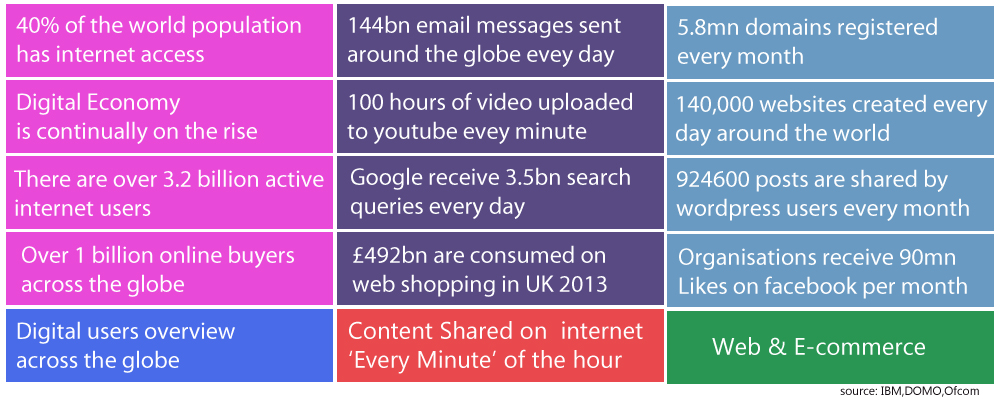
\includegraphics[scale=0.4]{chapter1/figures}
\caption{Data Facts \cite{ons}}
\end{figure}

Similarly, with such a huge volume of data, as shown in Figure 1.1, it is getting difficult day by day to analyse business and consumer behaviour. There is a greater need for analytical tools to help decision makers to understand data properly - there is no better option than information visualisation to understand and explore large amounts of data. The understanding of data will lead to the identification of trends, effective resource utilisation, educated decision making and understanding business and its core values (success and failure anticipation).

\section{Background of the Problem}

A brief summary of existing technologies in the area of research is introduced leading to the next section where the knowledge gap has been highlighted and introduced. 

Cloud based systems are gaining popularity amongst individuals, institutes and small and medium sized businesses across the globe - exploiting the Web 2.0 true potential. Web 2.0 focuses on the content which is mainly produced or created by its users \cite{3}. Similarly, data mashup systems are getting the same reception from various small and medium sized businesses on the World Wide Web \cite{patel2014enhance}. The industry leading companies such as Google, Yahoo and Microsoft are providing free cloud based services, including emails, mapping tools and cloud based storage. 

A mashup application can be characterised as a lightweight (simpler and faster) and a tactical (competitive activities) presentation layer that uses the web platform – Web-Oriented Architecture (WOA) - in order to integrate multiple sourced applications into one web-based offering \cite{4}.

Enterprise 2.0 contributes greatly to the process to generate, coordinate, collaborate and communicate content, applications and data in the business and enterprise environment. Enterprises such as small and medium sized businesses require tools which could address their core values (success and failure prediction), but also assist in decision making and providing extensive research based solutions from the existing data streams which will lead to effective resource utilisation;  not much has been done to answer these burning questions \cite{5}. 

However, information visualisation and data analysis is a field which holds the key to taking any business to the next level (expected and unexpected outcomes readiness). A business could do well and produce some quality figures in sales, but after all, it is about the techniques, how sustainable the practice is, and what further could be learned. Information visualisation converts data into interactive interfaces in order to easily understand problems, hidden patterns and scope and to explore data with a  more rapid and intuitive approach - usually abstract data are transformed into visual images to see the big picture at a glance \cite{6}.

In addressing data problems, a number of techniques \cite{7,8,9,eick1999visualizing,11} have been presented to explore data for trends, patterns and data exploration. Solutions such as pixel-oriented visualisation \cite{12} and pixel bar charts \cite{14} are available but these tools do not help with in-depth data analysis. The outstanding theoretical model which was introduced by Fry \cite{fry} is the most complete data analysis model, however the procedure is very complex and difficult to adopt without taking help from specialists on a regular basis to process data.


\section{Statement of the Problem}

The primary focus in business analytical tools or in information visualisation is on understanding data. The simple visualisation models are shown in Figure 1.2; these are basic visualisations of data included with software packages which serve basic data analysis needs. The in-depth data analysis is missing in such packages or applications. However, complex visualisation models are the outcome of research, mostly at a high level or through scientific experiments; these models provide in-depth analysis, but are very hard to practice in an enterprise environment. The main reasons are the simple visual representation, integration and compatibility issues which make it extremely hard to use the same tool for different organisations. 

\begin{figure}[H]
\centering
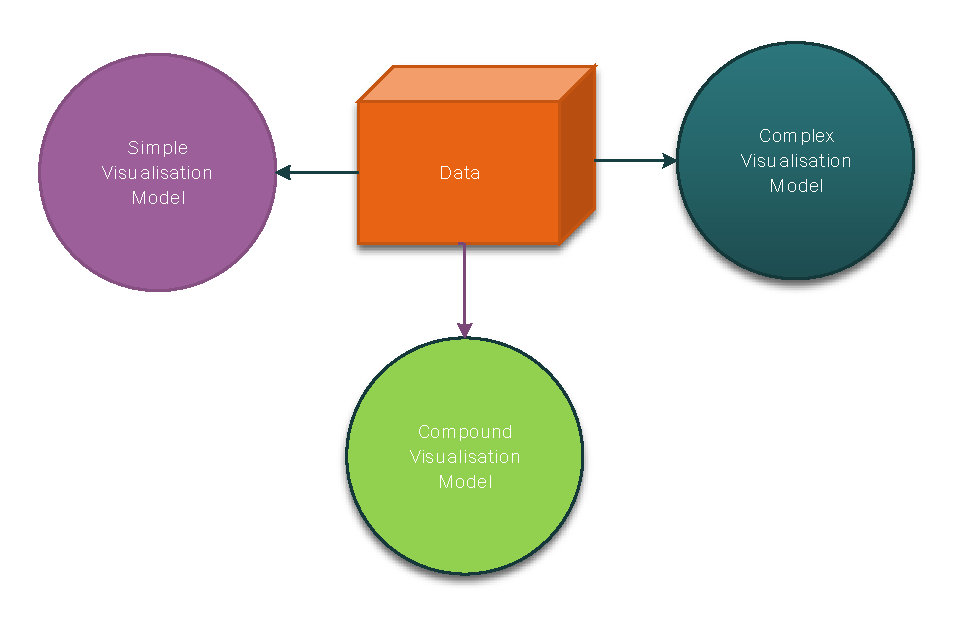
\includegraphics[scale=0.7]{chapter1/compound}
\caption{Visualisation Models Classification}
\end{figure}

However, very few visualisation models provide comprehensive solutions, but more importantly these solutions are hard to put into practice by small and medium sized businesses or individuals. There is a greater need for a compound visualisation model which is based on the concept of ease of use and integration while at the same time providing all the rich features present in complex visualisation models as there is a major knowledge gap in terms of data analysis and the human computer interaction. The research will focus on non-aggregated,  multi-attribute, multi-dimension and multi-coordinate visualisation and linked data visualisation thus making it a tremendous task and a very fresh approach in information visualisation, because the greatest contribution of information visualisation tools are to make it possible for the decision makers to identify the expected and discover the unexpected \cite{12}. Analysing complex data in a simple visualised form could be achieved through the proposed visualisation model.

\section{Purpose of the Study}

The aim of this research is to develop a data mashup system which will represent highly complex data in a simple visualised form for data analysis purposes used by businesses, individuals and government institutes. The system is targeted to reduce the technical requirements, such as data processing and data visualisation. Decision making within the system is accomplished by using a built-in pre-developed logical set of rules based on the data types and their sources. The architectural design will be so versatile that each data element could be utilised in the visualisation process upon request from the user for analysis and reporting purposes. 

\section{Objectives }

Some of the key research objectives are highlighted below.

\begin{itemize}
\item Data Analysis: 

In the recent past acquiring data was a long winded and painstaking process and one that had to be done manually. One of the main objectives of this study is to introduce an engaging and easy to use data analysis system which quickly analyses data and converts it into useful information. Data analysis and visualisation combine and form a perfect tool for the end user to understand and explore trends in large and complex data sets.

\item Information Visualisation:

Information visualisation is an act in which an individual establishes a strong connection between an internal construct and something to which access is gained through the senses. There are many types of visualisation approach introduced in the proposed system, but the following are major types which cover the unique aspects of this system and methodology. 

\item Multi-coordinate Data Visualisation:

Most software visualises data but very few display the same data in multi-coordinate views to investigate or to analyse business transactions more easily and cannot detect the failures and appreciate the accomplishments.

\item Non-Aggregated Data Visualisation:

Data visualisation practice is focused on aggregated data feeds, thus making it very difficult for the decision makers, or analysts, to find shortcomings or successes. The non-aggregated visualisation will enable users to capture unique insights about complex data in a more exhaustive analysis.

\item Multiple Attribute Data Visualisation:

The multiple attribute data techniques will visualise data with more than one data element and will help users to analyse data from different angles. This approach will help visualising multiple attribute data with coordinated visualisation for a thorough information analysis.

\item Transactional Tagging:

Tagging is widely used with social network sites, but enterprise tagging lacks research and contribution. This area needs to be investigated and business transactions need to categorise when they have successful or unsuccessful elements through data analysis and future re-use.

\item Interactivity:

Data and human computer interaction are two important aspects of any successful application. Data interaction is drilled down in the refining phase where various types of processes are applied to data to make it more meaningful for the end users. It is focused on human perspective – for example: layout, padding, proportional aspects, graph interactivity, scaling and zooming aspect of graphs for improving systems and data usability. There are many tools but a lack of user interactivity makes it very hard for businesses and individuals to get maximum usage of the systems - however the proposed system has introduced interactive and easy to use tools which give engaging overviews to the end users once the data has been processed through the data analysis phase and then visualised for the end user through data representation. The interactivity layer of the system is the bridge between the user and the application for complex analysis of data. 
\end{itemize}

\section{Significance of the Study}

This research will be a significant contribution to understanding complex data through information visualisation. The study will also be beneficial to individuals and organisations. In exploring and finding hidden trends through the high volume and complex data sets which will lead to interesting factual findings about the resources used for an activity. The significance of the subject has been divided into the following sections to give a brief overview of the research and its outcomes.

\subsection{Importance of the Study}

The data processing and storage capacity have tremendously increased; even a single transaction in a business creates many additional associated attributes. However, these attributes or data elements are not utilised directly in the business activities. The small and medium sized businesses struggle to cope with the analysis of such large amounts of data collected through various systems for the business - therefore small and medium sized businesses need a robust and easy to use and integrate visualisation system to explore and find hidden trends to help in making business decisions based on the data orientation - usage of the system is not limited to SMEs, it could be used by governmental institutes, organisations and individuals.

\subsection{Implications of the Study}

In most cases, small and medium sized businesses do not have enough resources to analyse and process collected data to explore trends and facts. The process is not easy and requires extensive data processing; however, if the collected data by any business is not analysed properly, then the actual scope of the business would be hard to identify. The comprehensive analysis of the data leads to informed decisions about the current status and provides predictions of future status - without data analysis decision making or business predictions are extremely difficult.

\subsection{Link to Existing Knowledge}

The proposed information visualisation system works closely with existing technologies such as data mashup tools for the interactivity layer and representation layer elements. The theoretical design has been derived from computational information visualisation \cite{fry} with more optimised steps both for enterprise and non-enterprise data types. The highlight of the research is based on the data representation layer, as many options are provided to the users to see visualised data in many formats and style to understand the data properly. 

\subsection{Industry Perspectives}

The visualisation model for both enterprise and non-enterprise environments brings numerous positives to small and medium sized businesses and individuals including government firms and organisations with extensive data usage. Information visualisation and data analysis bring diversified perspective about resources and outcomes. What assets of the business are bringing value to the organisations and what are the under performing assets which require attention in order to be fixed or adjusted? What are the best selling assets? What are the underselling assets? What assets require further improvements? Who are the best performers in the company or in the team? What are the current and future expected problems these assets might have? The answer to all these questions and many more bring amazing perspective to businesses and data related issues. 

\subsection{Impact on Policy Making}

Whether it is business or national policy - there are a combination of rules, plans, actions and conditions which are based on knowledge and information derived from existing techniques. All elements of policy, whether regarding its adaption or the formation of policies, are closely related to information and most of the information is generated through analysis of data through information visualisation; therefore information visualisation and data analysis play a vital role in policy making, especially for small and medium sized businesses and governmental organisations.

\section{Research Question}

The primary research question is the understanding of data through information visualisation. Enterprise 2.0 has the resources and ability to store and create a huge amount of transactional data, as Fry \cite{fry} highlighted that data and the purpose for which it was collected could be quite easily disassociated in such situations, and as a result we ask: if there is too much data, how can we understand it? 

In information retrieval systems and visualisation tools, the more specific questions users ask, the more specific and clear visualised results can be achieved, the existing techniques (\cite{7,8,9,eick1999visualizing} etc) are either developed with complex interactive and data representation or they are simple to handle complex data problems, as explained in the  problem statement above; this problem could be addressed through the compound visualisation model which gives extensive data representation to end users and the system is equipped with an interactive layer for users with no technical abilities powered by an extensive data analysis model.

For example, how many visits does a website receive? To answer this simple question, the user does not need information such as user IP address, screen resolution, browser and all the additional information stored within website statistics, but if the question is slightly changed to: how many visits does a website receive from the UK?, then users need additional information such as the IP addresses to answer such questions. Is it required to store all additional information, especially in an enterprise environment, because  users do not always know what factors are contributing towards a business success or failure. The solution does not lie with simple questions or queries but with analysing data and establishing relationships and links to data sources in visualised form.

\section{Research Design}

The concept of this research revolves around information visualisation through mashup application for enterprise and non-enterprise practice to understand huge transactional data for resource and decision making purposes, with the focus on understanding data through visualisation, interactivity of the system with the end user, storage of the generated results for re-use and comparison purposes and finally light-weight mashup applications - resource friendly and economical to run and operate. The theoretical model of the research is explained below and further explanations are provided in Chapter 3 (Research Design) and reference to existing tools and techniques are in Chapter 2 (Literature Review).

\section{Theoretical Framework}

The theoretical framework is based on four stages or layers starting with acquisition and data analysis to refine raw and complex data elements and generate information from them which is then passed onto the representation layer for representation of information in visualised form for end users. The interactive layer then creates the bridge between users and the system to customise or re-process information in various graphs and charts to explore data more effectively. The history layer enables users to store and explore generated reports for reference or comparison purposes. The proposed system is more extensively explained at the beginning of Chapter 3, which is further explained with experiments in Chapter 5 with UK postcode experiment while explaining with an advanced experiment on a business transactional data set in Chapter 6 and further experimentation in Chapter 7.

\section{Contributions}

The information visualisation model introduced in this research is a compact process for any size and type of data which is a major contribution in information visualisation and data analysis fields. Advanced data representation techniques are employed in Enterprise 2.0 using various data mashup technologies. New visualisation techniques have emerged from the research such as transactional tagging visualisation and linked data visualisation. The process and system is extremely useful in addressing complex data problems using an easy to interact and integrate with strategy. The contributions of the study are further discussed in Chapter 8.

\section{Further Work}

This research revolves around information and analysis through visualisation, as briefly explained in the introduction above; it produces results from complex data sets for small and medium sized businesses and individuals alike. However, like every system, there are some limitations in the data process and representation layer;  it depends on the nature of the data sets and the expected outcomes from complex and raw data sets.

The ability of the Visualixer system to process unstructured complex data for visualisation is a constraint as the system currently processes semi-structural data in a non-enterprise environment - the environment where data structure is not in a known state. However, the proposed system serves its purpose in an enterprise environment with the scope for improvement in data selection and versatility. The representation layer could further improve through more interactive graphs being added to the library. On-demand information, analysis and visualisation in a non-enterprise environment for non-relational data are usually not easy to represent in visual form. This could be addressed with further work and development. The mobile application of the non-enterprise visualiser will give freedom for mobile users, as mobile application usage is increasing tremendously. The non-enterprise visualiser is a cloud based system but added responsive features will add more value and will target a broader audience across different platforms. Further work and scope are highlighted in the final chapter of the thesis.

\section{Summary}

The overall structure of the thesis is highlighted in this chapter, the focus being mainly on the research problem and its background with suggestions for potential solutions and initial system design; it also gives a brief overview of the research and outlined objectives and research contributions.

There are two extensive experiments in Chapters 5 and 6 - both experiments have analysed quite large sized data sets: one from Royal Mail postcode analysis; the other was an enterprise data set with data from various different departments, along with further experimentation, in Chapter 7.

The literature review chapter gives a detailed overview of the technologies used in the research while Chapter 3 explains the theoretical framework, followed by design with system flow charts and expected outcomes while each section was being thoroughly investigated. The next chapter is the literature review; all related technologies and areas are highlighted which were used in the development and operation of this research, the focus was on data analysis and data representation along with Web 2.0 and mashup applications.




% Chapter 1

\chapter{Literature Review} % Main chapter title

\label{Chapter2} % For referencing the chapter elsewhere, use \ref{Chapter1} 

\lhead{Chapter 2. \emph{Literature Review}} % This is for the header on each page - perhaps a shortened title

%----------------------------------------------------------------------------------------

\section{Introduction}

In the past decade the world has been the epicentre of an extraordinary information explosion. This has been fuelled by the increased use of the internet coupled with the increased numbers of connected devices worldwide.  This rate of data growth has accelerated much faster than at any other point throughout history. This has affected not only machine generated data, but also enterprise application data - as both have continued to grow exponentially. This has posed industry experts with a great challenge - to develop new and innovative ways to evaluate and benchmark hardware and software technology and products. The studies have estimated that the total amount of enterprise data will only continue to grow \cite{gantz2012digital}. Data explosion not a singular incident. Its a global phenomenon that is growing every day. For example, with Asia now rapidly emerging as a major source of not only the data users, but also data generators. Similarly, with the increase of penetration in data driven computing, web and mobile technologies and enterprise computing, the new emerging markets have the potential to further add to this immense data growth \cite{kambatla2014trends}. 

The 21st century's global economic structure is transforming from an industrial economy into a new service economy. According to the results of a survey done by World Bank, the output of this service industry model takes up over 60\%  of the output in the world (sometimes exceeding 70\% in developed countries). This is partly because competition within the service industry is fierce, and this has become a huge focal point in the world's economic development. This means that service computing which provides re-usable architectures to support the modern service industry has come under the spotlight, and turned into an incredibly promising research area. Coupled with the increased popularity of cloud computing, more and more modern services are being deployed within cloud infrastructures in order to provide rich functionality. The number of services and users increasing every day, this has fuelled the explosion of data generation seen through services including mobile devices, social networks and large scale service oriented systems. It is because of factors such as these that the sheer amount of service generated data has become too large and complicated to be processed effectively by the more traditional approaches \cite{worldbank}.

It is no surprise, big data widely recognised and has attracted attention from the government, industry experts and academics. This is because big data is full of high volume, high velocity and variety information assets, and the increasing data requires new forms of processing to enable and inform enhanced decision making, insights, discoveries and further process optimisation. This issue was even mentioned by the Compliance, Governance and Oversight Council (or CGOC, which is an organisation focused on information governance) \cite{manyika2011big}. It is mentioned that, on average, information volume doubles every 18-24 months for most organisations, but the data creation speed is tremendous \cite{chen2014big}. In fact, its such a hot topic that in 2012 the Obama administration announced the big data research and development initiative, which explored how big data could be used to address the important problems facing modern governments \cite{wu2014data}.

The reaction to this phenomenon from leading IT companies such as SAGE, Oracle, IBM, Microsoft, SAP and HP has been staggering. These organisations have spent astonishingly on buying new software firms that specialise in data management and analytics. Data analytics industry on its own is worth over \$125 billion, and is growing at a rate of almost 10\% a year (this is twice as fast as the entire software industry). Because of this shift, effectively and efficiently creating values from big data has become an important research topic \cite{gantz2012digital}.

The emerging service oriented systems are not simple and often involve a huge number of services, each with complex services. The big data generated from these systems is typically heterogeneous, as well as being of multiple data and incredibly dynamic. And due to its nature, the increased system size and volume of data it contains, creating value from this became an incredible challenge. A few examples of the service generated big data being produced includes, trace logs, quality of service information and service invocation relationship. While similar to other kinds of big data, service generated big data initiatives span 4 unique dimensions \cite{ecoweb}:

\begin{itemize}
\item Amount: Modern large scale systems are full of every growing amounts of data which easily amasses terabytes and even petabytes of information.
\item Momentum: Certain time sensitive processes (such as bottleneck detection or quality of service predictions) could in fact be achieved as streamlined data streams directly into the system.
\item Variety: Both structured and unstructured data are generated in various data types, and this makes it possible to explore fresh new insights when analysing data in groups.
\item Collection: Detecting and correcting noisy and inconsistent data are important factors when constructing secure and trustworthy analysis. Establishing trust in big data presents a huge challenge, especially as the number and variety of sources continues to grow.
\end{itemize}

These four characteristics are unique to service generated data, and it provide the greatest challenge for data management and analysis. In order to achieve the full potential of this service generated through big data, developing exceptional technologies to effectively process large quantities of data within shorter processing times is a critical task. The transactional data or data sets utilised in this research is a kind of sub-set of big data phenomena, as the data sets are quite complex and the contributing sources are alike, the solution presented in chapter 3 could also be applied to any kind of data. 

\section{Acquisition and Data Analysis}

In the recent years getting data was a complicated and painstaking process and one that had to be done manually. For just a single voltage reading an engineer would need to go into the unit, manually attach a digital multimeter to the connections. The results would then need to be written down along with measurement values. The more complex the reading needed to get (for example a continuously varying signal voltage) the more difficult it is to read and measure accurately. Instead of just attaching the digital multimeter and taking reading, one would instead have to remove the original connection and instead connect to a separate standalone oscilloscope. And while it was possible to perform a visual inspection of the signal and perform a rudimentary analysis, it was challenging work. And not only was it a long and difficult task, it was made more difficult by the fact that each instrument was independent of the others and the limited available technology. However, the upside to this was that data management was a relatively easy task and our modern issues of volume and speed simply were not a problem \cite{mesurementsystems}.

There have been both major strides forward in technology and a significant decrease in the cost of hardware and software. Improvements such as the increase of microprocessor speed and storage capacity have helped form the catalyst for an explosion of data, one that is still increasing in size and speed every day. Now, the days of independent instruments are a thing of the distant past, with automated measurement taking over with hundreds of combinations of measurements and new devices that can function as a single cohesive system, instead of in multiple parts. It is because of these spectacular new developments that can make new discoveries and formulate new scenarios. Data acquisition rates have skyrocketed; peaking well within the mega-sample per second range every day, and technologies like high channel count systems are available to everyone. Data acquisition has become a profitable business in its own right and now there are even a range of affordable bench top data acquisition systems \cite{di2013data}.\\

In a nutshell, hardware concerns have been reduced along with primitive data collection tools. Recently, instead of focusing on the hardware vendors are now working to accelerate data collection even further, enabling engineers to break through previous data rates and resolution barriers. Worryingly, this has all happened so fast that it has inadvertently triggered a whole new wave of software issues to contend with. Instead of the previous hardware issues and the data, engineers are faced with unassailable mountains of data \cite{mininghighspeed}. The new technology provoked richer and faster data retention. The race has changed pace; now it is not about who can collect the data fastest, but who can make any sense of it \cite{chen2011essential}.

A growing number of modern technologies and complex products require data acquisition throughout nearly every stage from design and development to verification and testing. This means that engineers are facing the challenge of testing increasingly complex and delicate designs within smaller time-frames and ever shrinking budgets; all to meet the rising demand of customers who want high quality products for low prices. This means that quite a significant investment needs to be made in data collection to make the effort viable. There is hardware to consider, plus automation systems and the personnel need to perform tasks and analyse the data - which is still streaming in increasing volumes \cite{storager}.

Hand in hand with the huge volumes of data being collected comes the need to analyse it all and it is not something that has gone unnoticed by businesses. During the last decade business interest in data analysis has skyrocketed, and its not hard to see why. The competitive advantages a business can gain from analysing such data is huge which can provide decision makers with a solid grounding for decisions \cite{basicbusiness}. However, a business may want to implement sweeping changes based on the analysed data; the physical ability for change is limited by many other factors; such as staff knowledge, business supporting systems. This means that when a business depends on enterprise information systems, to modify or replace supporting information systems in order to make changes to business practice. Not to mention the most significant change modifying operational information systems is a must and these are often located within central repositories of automatic summarised data within huge data warehouses. That's why making changes based on data became a lot more complicated \cite{garcia2014using}. In the next sections, various web mining techniques will be analysed which will later be used in the system design and development process. 

\subsection{Web Mining}

Web mining is a technical term relating to the application of various data mining techniques to discover patterns and trends from the internet, and from a variety of enterprise data sets that are available to mashup applications. There are many different definitions of web mining, the definition found within the Gartner Group is the most comprehensive. Data mining is the process of discovering meaningful new correlations, patterns and trends by sifting through large amounts of data stored in repositories and by using pattern \cite{larose2014discovering}. Data mining is the process of uncovering hidden trends and patterns (that lend towards predictive modelling) and using a combination of explicit knowledge bases, sophisticated analytical skills and academic domain knowledge. This is also known as the process of producing new observations from pre-existing observations \cite{raju2014data}. This has also been described as the process of automatically extracting useful information and relationships from immense quantities of data. However if the purist approach is adapted, data mining does not involve looking for specific data; it simply finds patterns that are already present. This means that data mining cannot be used to unearth information in response to a question or hypothesis \cite{larose2014discovering}.

The continued increase in growth of online information combined with the unstructured nature of web data requires the development of powerful and efficient web data mining tools. Instead web mining tools are designed to dig out useful facts and knowledge from web pages, hyperlinks, page content and usage logs. It can be used in a number of ways to enable the streamlining of business process. For example, the web mining of an e-bank service can enable the employees of a bank to support e-business, helping to understand various marketing dynamics, new promotions or suggestions on the internet. Because of this there is now more of a tendency amongst banking companies and individuals to collect banks of information through web data mining, and to use that information for own interests to gain business intelligence, and this helps to make enlightened business decisions \cite{raju2014data}. Figure 2.1 shows various web mining types which are further discussed in the chapter.

\begin{figure}[H]
\centering
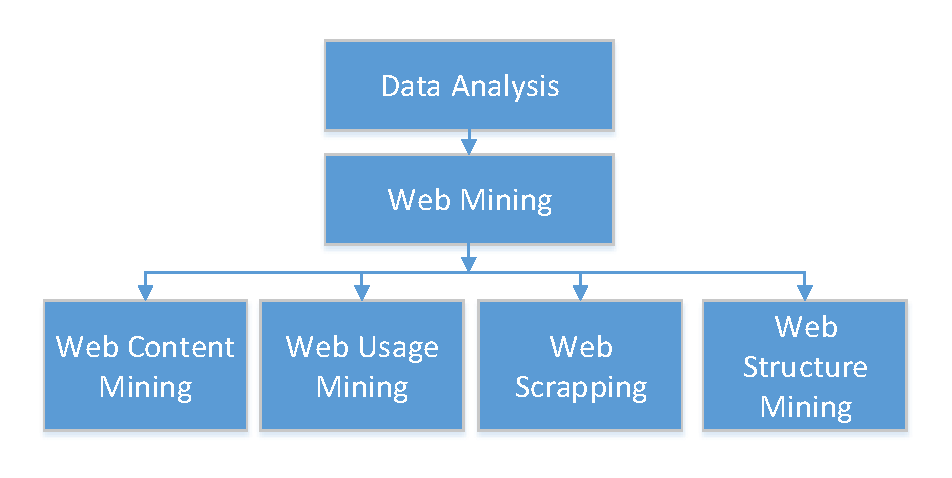
\includegraphics[scale=0.8]{chapter2/webmining_types}
\caption{Web Minning Overview}
\end{figure}

Web mining techniques are the result of an incredibly long process combining years of research. The web mining existed when the business data was first being stored on computers and on the internet, and evolution continued with drastic improvements in data access, and now the developments in real-time technologies that allow internet users to navigate through data quickly \cite{gargi2014dynamic}. Data that is gathered from surveys, manual input or from independently networked locations to define the data collection. Semantic Web has been developed to address current web problems, and it does this by methodically structuring the content of the internet and adding semantics before extracting the maximum benefits from the power of the internet. Sir Tim Berners-Lee defined the semantic web as an extension of the current web in which information is given well defined meaning, better enabling computers and people to work in co-operation \cite{berners2001semantic}. It is, in a word, a vision. The idea of having all of the data on the web systematically defined and linked together in a way that can be used and understood by machines. And not only for display purposes, but for automation, integration and the reuse of data across a whole liturgy of applications. Web mining also plays a pivotal role in achieving this, as it lets users quickly and easily find the information required.

Web based documents are split into three categories based on the structure: un-structured, semi-structured and fully-structured \cite{kim2015dynamic}. Structure data is usually in a normalised form such as databases \cite{park2014crowdfill}. Semi-structured data is not in a normalised form but contains markers or tags \cite{mansmann2014discovering}. Un-structured which doesn't have any pre-defined data model. There have been research studies into these categories, specifically on un-structured and fully-structured data, to look into the methods of  extracting semantics for ontology learning. In the research that focuses on fully-structured web documents benefits from a standardised syntax such as XML. However most of the web documents in existence today are in a semi-structured format, but only a few references are made to research that specialises in this format in extracting semantics for ontology learning. In most cases the plain text has been extracted from the semi-structured pages in pre-processing, therefore neglecting embedded information within the semi-structured format. Some other researchers focus on extracting semantics from more template driven web pages, and so these methodologies are limited both in usage and applicability \cite{liu2007web}.

\subsection{Web Usage Mining}

The term web usage mining was coined by Cooley \cite{mobasher2000automatic}, and is the application of various techniques used in data mining to discover and analyse the usage patterns of web data. It analyses user interactions with web servers including web logs or other database transactions from a group of related sites. However it has sparked privacy concerns and is currently the topic of much passionate debate. This is because the process includes mining data from the web server access logs, proxy server logs, browser logs, user profiles, registration data, user sessions or transactions, cookies, user queries, bookmark data, mouse clicks and scrolls and any other data as a result of interactions. Its aim is to discover the general patterns in web access logs, but in order to discover these patterns it is necessary to perform a few processes, including pre-processing, pattern discovery and pattern analysis \cite{wang2015design}. Web servers automatically record and store data about all of the user interactions whenever requests for resources are received. Analysing these web server logs, all kinds of different websites can better understand user behaviour and web structure, which in turn improves the overall design of this immeasurable collection of resources. Mining web usage pattern data, user can help in the progression of internet based studies; including those based on how internet browsers are used, and how the users interaction with the browser interface changed. These patterns can be put to use in gathering business intelligence, which will in turn improve customer attraction, retention and other aspects of customer behaviour \cite{claiborne2015self}.

\subsection{Web Scraping}

Web scraping is defined as the technique of automatic web data extraction, used in order to extract data from the core HTML of the website by parsing (the scouring and analysis) the web pages \cite{o2009web}. It does this by using programs specially coded for manipulation of web pages. Examples of this are: converting the web page into another format such as XML, or by embedding the browsers. It can be seen as fairly close to web indexing (this indexes web content using a soft-bot mainly adopted by search engines) but instead web scraping focuses on the transformation of completely unstructured web content into formally structured data, which can be stored and analysed in a central database. 

It can be used for a multitude of things, including online price comparison, weather data monitoring, web research, web content mashup and wed data integration. Not only that, but it can provide various levels of scrape like human copy and paste, text gripping (based on the UNIX command or regular expression matching facilities of programming languages like Perl), HTTP programming (HTTP requests to the remote web server), embedding web browsers, HTML parsers and web scraping software tools. A web server can be used to process to the scripting language, which in turn will produce the HTML response. Utilising text grabbing one can use the regular expression matching technique (where try to match a particular expression in the file) and find a match. Once a match has been found for the expression, users can then pick the values before or after it. The main limitation of scraping programs which are required to update frequently, which can increase the maintenance costs \cite{munzert2015automated}.

\subsection{Web Structure Mining}

Web structure mining is a field of research entirely focused on identifying more preferable documents by using the analysis of the web link structure \cite{kosala2000web}. The idea is simple: a hyperlink from document A to document B implies that the author of document A thinks that document B contains worthwhile and useful information. Web structure mining seeks out and exploits the additional information that can be found within the structure of the hypertext. Because of this one of the most important application in this area is the identification of the relevance of these linked pages which appear equally important when analysed, especially when one look at the content in isolation. To illustrate: a hyperlink induced topic search analyses the hyperlinks topology by discovering authoritative information sources for broader search topics. To find this information, it goes to authority pages, which are defined in relation to hubs as the counterparts. Hubs are otherwise known as pages that link to multiple related information authorities. For example, Google owes its massive success to its page ranking algorithm, which states that the relevance of any page increases with the number of outbound links (hyperlinks to it from other pages); more so if those other pages are relevant \cite{renu2014implementation}.

\subsection{Web Content Mining}

This is an automatic process of the internet which extracts patterns from web contents, data and documents (such as HTML files, images or emails). This already goes beyond simple keyword or key phrase extraction; instead it can take full advantage of the semi-structured nature of the web page text, and can use it to detect co-occurrences of terms within the texts. For example, user can also discover  trends over time, which could indicate a surge or decline of interest in certain topics (such as the programming language Java) \cite{mobasher2000integrating}. Another area this can be applied in is event detection; using web content mining in the identification of stories in multiple continuous news streams that correspond to new or previously unidentified events \cite{yadav2015web}. 

\section{Data Representation}

Visualisation has been a prominent and fast moving field for a long time, as a sub-field within science, statistics and graphs, it has only been recognised as its own entity since the mid to late 80s \cite{wilkinson2009history}. In this field, the full depth of the seminal work conducted, the strength of visualisation is drawn from its background; years of statistics and graphic design that form the basis for something much stronger. The process known as information visualisation is done by converting data into a series of interactive interfaces to allow users to understand data problems, unearth hidden patterns and explore the data with a more intuitive and analytical approach. Traditionally, visualisation uses aggregate data and transforms this into visual images, to allow users to see the big picture at a single glance \cite{chen1999information}.

Information visualisation is a process, also known as a visual medium between data and the people trying to understand it. It also works as a bridge to establish interactivity between source and operator for analysis and decision making purposes. The ultimate goal of information visualisation tools are to provide and improve data perception, correlation, interpretation and exploration. Setting apart good and bad practices in information visualisation can sometimes be difficult to define the parameters in order to establish quality visualisation. These are key visualisation attributes \cite{carr1999guidelines}:

\begin{itemize}
\item To analyse or examine entire data set.
\item Ability to see non-aggregated elements of subsets.
\item Customisation and filtering to analyse data at multiple degrees.
\item Making additional information available to an action which is performed by the user.
\item The ability to relate data items with similar characteristics to form and build relationships.
\item The ability to undo an action made and show the steps performed up to the current point. 
\end{itemize}

In order to analyse data problems in depth, a number of different techniques have been invented to explore data \cite{wang2000guidelines, north2000snap,pillat2006coordinating,eick1999visualizing,stolte2002polaris}, allowing users to dig deeper and find trends and patterns. For example, both Tableaus visual spreadsheet \cite{tableau} and SpotFires visual data exploration interface \cite{spotfire} are utilised by business managers for routine data analysis. The existing visualisations tools such as pixel-oriented visualisation \cite{keim2002pixel}, where large transactional data sections are represented by each pixel in the visualisation, digging into data to explore patterns and trends. For example, in the VisDB system \cite{keim1994visdb} each individual pixel is arranged and coloured to indicate the items relevance to a user query. Equally well known technique that uses pixel-level visualisations the Seesoft software visualisation technique. This technique maps each line of source code and connects them to a line of pixels. These techniques have been used in a wide variety of ways including to build interactive decision tree classifiers, which would be based on the visualisation of training data \cite{eick1992seesoft}. Another approach to non-aggregated data visualisation is known as value cell visualisation \cite{keim2007value}, and this is usually displayed in bar chart format. Pixel orientated visualisations became a necessity within data visualisation in part because all other visualisation practice (such as pie charts, bar charts, x-y plots) are a form solely focused on the aggregation of data, which in  turn restricts the number of data values able to be visualised. While this is a working model, this dilutes our understanding of the data and the visualisations do not always give the precise and accurate information to the decision makers. The pixel bar charts and value cell bar chat visualisations were a fantastically successful way to visualise non-aggregated data, but this left a lot to be done in terms of multi-coordinate data visualisation and data relation in visualised form - with a lot of gaps still in the process. Using multiple view systems, can use two of more distinct views to support the investigation process of a single entity. However a view is only considered distinct when compared to other views if it allows the user to learn the different aspects of the conceptual entity - whether by presenting different data or by emphasising different aspects within the same data  \cite{keim2002pixel}.

The Snap-Together \cite{north2000snap} is a data analysis and information visualisation system that supports the use of several different types of data set. The coordination of this data is limited to the selection of data items the DEVise can represent, and multi-dimension data is separated by the DEVise into several multi-dimension visual representations. Users can then move on to view integration, which is accomplished by zooming in and using multi-coordinate views on the data to explore it further.  This view supports a coordinated series of data items, and is recognisable by a selection, highlight and colour mapping dynamic queries of the data. Approaches such as this multi-coordinate visualisation provide a solid understanding of data, and helps in the data validation and cross examination of data to find hidden patterns and trends, as well as providing critical information to the decision making process. However, when trying to see the original data even these multi-coordinate practice fall short of the mark. In order to resolve this, the proposed linked data visualisation which provides a link and relationship between different data aspects \cite{abraham2014multi}.

It is often said; a pictures worth a thousand words. But does such an intelligent analytic speed imply that people can absorb visual information in a more efficient way than information conveyed through words? Can we happily say, for example, that people learn and remember visually presented information better than they remember verbal information? There have actually been a number of experiments that have tried to demonstrate this very fact, with mixed results. Some authors find no significant link between presentation style (visual vs verbal) and recall rates unless individual preferences are taken into account \cite{butler1996multimedia}, on the other hand visual business intelligence is on the rise, analytical tools are becoming mainstream \cite{basole2014visual}. However, according to studies visual intelligence is the most dominant type of intelligence, and many researchers and teachers surveyed \cite{survey1} believe that most of the students learn best through a visual medium.

\begin{itemize}
\item  approximately 65 percent of the population are visual learners; 
\item the brain processes visual information 60,000 faster than text; 
\item 90 percent of information that comes to the brain is visual”. 
\end{itemize}

Why does it appear that we understand words/numbers and graphs differently? People interpret numbers and graphs differently because these are processed differently in the brain. Numbers and words are generally handled by the verbal linguistic system and graphs are handled by both the non-verbal linguistic system and the limbic system. The bit rate of the visual system is about 10 million bits per second \cite{koch2006much} and the rate of reading is approximately 150-400 words per minute. To understand how this works, and provide a foundation for further reading, a very brief review of the relevant neuroscience seems in order. Following are some neuroanatomical details of the human brain. However, there are many other important aspects of cognition such as perception, memory, emotional modulation.

In the digital age, and there are huge volumes of data and information available within organisations, which if handled incorrectly can lead to data paralysis. To avoid this, it is increasingly important for organisations to ensure they are using the information effectively and that includes using data visualisation to explore and present the information. Information visualisation is the perfect way to present data graphically and take advantage of the visual nature of people allowing users to amplify cognition and gain better results. Through visual stimulus. The information visualisation used within the Spotfire \cite{koch2006much} and IBM Cognos software \cite{ibmcognos} provide visualisation techniques such as histograms, bar graphs, scatter plots and tree maps. These visualisation techniques are used in computerised environments in order to amplify human cognition in 5 key ways:
\begin{itemize}
\item  Increasing the memory and processing resources  available to users;
\item  Reducing the search for information;   
\item  Enhancing the detection of patterns;   Enabling perceptual inference operations; 
\item  Using perceptual mechanisms for monitoring  systems;   
\item  Encoding information in a medium that enables  easy manipulation.  
\end{itemize}

As discussed above, the information visualisation science is such an important contribution in learning fast, the same principle could be applied with learning from complex data. The next section of this chapter will discuss various types of visualisation which will be introduced in the research model for greater understanding of data problem.

\subsection{Bar Charts}

In terms of presentation graphics, bar charts are certainly the most simple and effective method, however it can only show aggregated values such as total sales for each months, making it limiting. Because of this, valuable information often gets lost in translation and is difficult to analyse. In fact, the usefulness of bar charts is especially limited if the user is interested in exploring the relationships between the different attributes available such as product price, number of orders and quantities.  The reason for this limitation is that multiple bar charts for different attributes do not support the discovery and exploration of interesting subsets which is one of the most important elements of data mining. A number of visualisation techniques have shown that the usefulness of data exploration in the discovery of patterns and trends is key in multi-dimension data. For example, both Tableaus visual spreadsheet \cite{tableau} and SpotFires visual data exploration tools \cite{spotfire} are widely used by business managers to aid in daily decisions making. Space filling techniques such as squarified treemaps and screen-filling curves are also used to help visualise hundreds of data records daily. For the aid of visualising even larger amounts of data, pixel-oriented techniques (which, as explained above, use each pixel to represent one data value) can be used for effective understanding. In the VisDB system \cite{keim1994visdb} for example, each pixel is arranged and coloured to indicate an items relevance to a user query. However, bar charts used with a combination of other simple charts exploration data could help in addressing data problems.

\subsection{Multi-coordinate Visualisation}

Multi-coordinate view is a very specific term for the exploratory visualisation technique that enables users to explore the data in full. The overall idea for the technology and premise for the technique is that it helps users to understand data better in a presented form displayed in various representations to allow an overall image. On the one hand, users want to view complex and intricate data in a simple way of exploring and deciphering, discovering facts and patterns that aren't easy to find. These complex data investigations require the user to consider many different scenarios in order to compare the visualisations generated from multiple data sets. To aggregate and mine such vast arrays of data, sometimes fusing data from many diverse data sets and create new information and insights, while still maintaining the ability to roll back to the previous incarnation, can be a difficult task. This is especially true when experts are looking at the same sets of data, but comparing and discussing different exploration paths and conclusions. Such complex and delicate analytic investigations require the right exploratory tools, allowing for a comprehensive analysis with intuitive functions \cite{roberts2007state}. 
On the other hand, some users might already be too familiar with the techniques these programs use, and because the applications on autopilot, missing out on some of the riches of the underlying data. Utilising a visualisation design environment which allows users to examine the different representations of the data while managing the interactions and automatically coordinating operations between the different views. Using this approach to open up new and insightful facts and relationship information about the users data without sacrificing accessibility.

In a nutshell, the purpose of a good visualisation application is to allow all users to have an interactive dialogue with the data. It can be quite challenging and time consuming to find, collect and make sense of large volumes of data, and how application makes the process of handling such data, even if it is from multiple sources of various types, much easier for the end user. The user's goal in this situation is simple to understand the data, view trends, find unusual patterns and organise this information in any way that is desired. Allowing unrestricted access to the data and its deeper meanings, and are able to discover and compare differences and similarities in the data sets, examine the outcomes of various scenarios and develop grounded theories through systematic analysis. In order to achieve greater insights to data problems, the visualisation systems should provide interactive visualisation experience. Which enables users to dig deeper and discover new meaning in the data. These interactive systems are the heart of the coordinated multiple views technique, therefore allowing insights through data analysis \cite{zhang2014visual}.

\subsection{Multi-dimension Data Visualisation}

The development of the modern database system, users can now find multi-dimension data is a prominent presence in a wide variety of fields. This is largely because individual people on own lack the time and skills to find multi-dimension data, limiting the knowledge and ability to visualise multi-dimension data to help in decisions. Creating an easy to use and highly interactive visualisation model that allows users to dig for knowledge within the data has become the main challenge within the visualisation field. The unique technology used within multi-dimension data visualisation is adopted primarily from the data mining area of visualisation. Such techniques are used as a communication tool, to help us generate the initial view, resolve complex structure issues and display the data and analytical results in order to give us a clearer perspective. However this is quickly changing \cite{mothe2003doccube}. The general scope for visualisation is a much more comprehensive collection of information, with many different techniques. In multi-dimension data visualisation, system has a number of display options which are viewed as the traditional paths - such as parallel coordinates, word shape or scattered matrix. These methods work perfectly for smaller amounts of data, but when to start moving into larger volumes these methods start to fail. The answer to this problem lies with multi-dimension data coordinates,visualising data in more than one dimension for trends and patterns exploration \cite{khandelwal2014multi}.

\subsection{Multi-attribute Visualisation}

The geo-spatial data sets, while often unstructured in nature, typically have size, distances, directions, locations and altitudes, giving an inherent positional structure and shape. But maintaining the boundaries of such spatial objects imposes major structural and positional constraints on our choice of visualisation techniques. The data associated with such spatial objects can often be multiple variate, making visualising such multiple variate spatial objects a very challenging task \cite{shneiderman1996eyes}. In particular, time varying geo-spatial data volumes are often so large that interactions among these become too complex, and it is often difficult for users to understand how the data changes over time when the individual images are viewed in isolation, so in order to show both spatial and temporal data changes over periods of time, special visual methods are needed to unearth the important patterns and relationships within the data \cite{maceachren2005visualizing}. These changes in the spatio-temporal data might be existential (such as appearance or characteristics) or it may be spatial (changes in shape or position) or even attribute changes ( such as changes in non-spatial characteristics of spatial objects). In this explanation, to deal with attribute changes within spatio-temporal data. Using more trajectory based techniques like those proposed \cite{skupin2000metaphor}. Users are able to represent changes in attribute as the movement of objects across a two dimension self organising map surface. The computational changes are made to complex data in order to distort the spatial locations, patterns are often more visible. In stark contrast, our application required these spatial location points to be preserved, not altered. Solcum \cite{slocum2001cognitive} suggests that spatio-temporal data that is associated with point locations can be displayed using animation, small multiples or changing maps, as evidences in the tool MapTime. However,  Andrienko mentions that animation is often not an effective method for analysing the change in attribute values, due to the effects of change blindness \cite{andrienko2003exploratory}. Skupin \cite{slocum2001cognitive} argue that the need for temporal visualisation methods for census data cannot be fulfilled simply by using multiple maps placed side by side, or by using percentage change maps. This is owing to the large size of census data, and it is imperative that the task of identifying change for visual detection is not left to simple human users. CommonGIS \cite{andrienko2002testing} offers multiple techniques for visualisation, where a coherent display of multiple maps is used to compare several different scenarios. In addition, CommonGIS also provides choropleth maps, time maps and time aggregates to visualise spatio-temporal data more effectively. However, with the execution of choropleth maps, most of the techniques provided in CommonGIS represent data by using graphs, time series charts, histograms and scatter plots. Instead our application aims to visualise information on the map while still maintaining the spatial boundaries of the planning polygons, since these are what help the user understand the data more effectively \cite{tahir2014geovisual}.

\subsection{Business Analytics Through Visualisation}

There are many definitions for the term analytics, with professionals in different fields viewing it in very different ways. However the common ground that may find, is that analytics is the processes of reviewing a set of insights generated from accurate historical data, and developing a series of actionable decisions of recommendations based on it \cite{melpignano2012platform}. Recently there has been a development from The Institute for Operations Research and Management Science (otherwise known as INFORMS) that has created a major initiative for the organisation and promotion of analytics. By the definition INFORMS present, analytics represents the combination of computer technology, management science techniques and statistics to help solve real problems. This has sparked many other organisations to develop the interpretations and motivations for the use of analytics \cite{keim2008visual}.

The descriptive analytics (also known as reporting analytics) refers to a detailed knowledge of activity within the organisation, and further to that the identification and understanding of the underlying trends and causes of the activity. To do this, there is a certain amount of data source consolidation and availability required to gather all the relevant data to analyse and ensuring that this is all in a form that enables reporting and analysis. This creates a data infrastructure, and user can use this to develop the required reports, queries, alerts and trends using the various reporting tools and techniques. This process and the technology used within it has become a key component in how user visualise and deal with data. Using the latest available tools in visualisation user can move on to developing accurate and powerful insights into the inner operations of our organisation \cite{haas2011data}. 

The predictive analytics is a process that sets out to determine what is likely to happen in the future based on trends. This form of analysis uses statistics as a firm basis, as well as newer techniques that have been more recently developed in the field of data mining. The goal of using these techniques in data analysis is to be able to predict the behaviours of customers likely to switch to a competitor company, how much of what they will buy next and what special offers or promotions would evoke responses. In developing these predictive analytical applications a number of techniques were used, including various classification algorithms. These included decision tree models and neural networks (similar to those used to predict box office success) and clustering algorithms (to segment customers for targeted promotions). Combining these with well known association mining techniques user can create estimations of the relationships between purchasing behaviours (what a customer is likely to purchase based on previous purchases). These analytics are essential to retailers in the process of promoting or recommending products for the customers \cite{shmueli2011predictive}. 

The third and final category of data analytics is known as prescriptive analytics - the aim of which is to examine both the current trends and the predictions made via predictive analytics, and use the information to make educated decisions. As a group these techniques are often referred to as operation research or management science, and are used to optimise the performance of any given system. The overall aim of this technology is to provide recommendations or provide a concrete decision for a specific action. Recommendations from this model can come in the form of yes/no decisions, defined amounts (if this was the aim, e.g. the price for a specific item) or even a complete set of production plans based on reports. The decisions created can be presented in either a decision making report, or used directly in an automated decision rules system (e.g. airline pricing systems). Because of this versatility, prescriptive analytics can also be known as Decision or even Normative analytics \cite{davenport2007competing}. 

There are hundreds of different ways one can measure and evaluate the success of a business. To use profit margins, staff performance rates or sales figures. But the most important way to do this is through simple client satisfaction. In some cases businesses will view this as more important than the business profit. However determining levels of client satisfaction is not as easy as it sounds and is instead determined by a specific sequence of information and decisions about the quality of services, offered products and getting to know the clients among others. This can be determined by predicting the needed improvement of infrastructure based on a client growth rate, defining the need for expansion with variety of specialised products, or by establishing detailed profiles of the clients, including which of the products or services are required, and when. The bigger question here has yet to be asked if the criteria are known and established, then why are so many businesses having trouble achieving the goals? Well, this could be something as simple as the fact that analysing such enormous amounts of data is by no means a trivial task and that the system reports generated from that data don't always hold the answers. It is because of this variable that the decision makers in charge often don't have enough information to complete the picture - or in some cases have gleaned incorrect information because the correct data is lost in an endless and overly complex report. Because time is such a critical factor in business decisions, being presented with a set of static data is also not the answer - as this can skew the picture \cite{bertsimas2014introduction}. The aspect every decision maker is striving to find a way to automate and manipulate the information harvested in an easy and intuitive way to make vital business decisions. This need sparked the development of new data mining techniques, which in turn generate new and innovative business information. However, it is not always as easy as it sounds. Because of this complexity, a set of visualisation tools are being developed in tandem, to help display the data in an easy to understand way. This will make it much easier for those decision makers to identify trends, discover new and unexpected turns in the market or the client base, and to find - new ways and processes to improve business opportunities further \cite{albright2014business}. 

\subsection{Data Mashup}

The term mashup refers to a new form of web application and presentation that are created by combining data from multiple existing sources \cite{gomez2004ontological}. Mashup span a wide variety of factors from simple visual aggregation of websites to rich internet applications, and combine very diverse sets of data. The easiest way to visualise it is this: think of a salad bar at your favourite restaurant. The vegetables on the bar are different data sources, and the bar itself represents a visual mashup (or aggregation) of the various vegetables. But the salad that you create represents a much more complex mashup, where the sources are combined in an interesting way to create something entirely unique and new. Typical data mashup architecture. Figure 3.2 shows the basic architecture of mashup system and its data sources.

\begin{figure}[H]
\centering
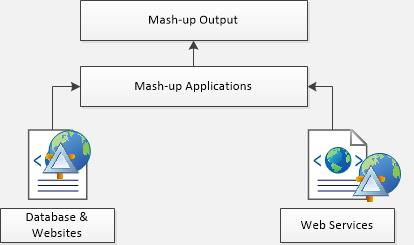
\includegraphics[scale=1.2]{chapter2/mashup_arch}
\caption{Data Mashup Architecture }
\end{figure}

There are many definitions used for mashup technologies, but in all definitions there are two consistent themes which are listed below \cite{fung2012service}.

\begin{itemize}
\item Mashups are very simple to create and easy to deploy. In fact, that business users should be able to create without any great assistance from the IT application developers.
\item Mashups are composed of a selection of easy to integrate data sources. These data sources could consist of either pure data formats such as XML, JSON or CSV, or a combined data and presentation formal (HTML).
\end{itemize}

Through these two themes user can see the basis of a disruptive technology. In this technology the need for agility and self service for the business users intersects with the existing technologies for easily exposing the desired data in an easy and understandable fashion. The mashup technologies span a wide variety of users - such as the consumer using a portal or rich internet app that collects, aggregates and transforms diverse data sets into something new. Mashup technologies also bring in data sources to expose the data and make it easily consumable. Here are the two points; first some of the methods that data is exposed from a structural and protocol perspective, and second some of the different aggregates and portals that are available on the consumer market \cite{arafati2014d}.

\subsubsection{Mashup Data Sources}

A mashup data source can be almost anything one can imagine including an in-house database, a web page or a web service. The main goal of a mashup is to easily consume data, to the point that a business user can create a mashup \cite{gomadam2012data}. This means that most data sources that are commonly used in mashups expose the data by one of the following mechanisms as illustrated in Figure 2.3.

\begin{figure}[H]
\centering
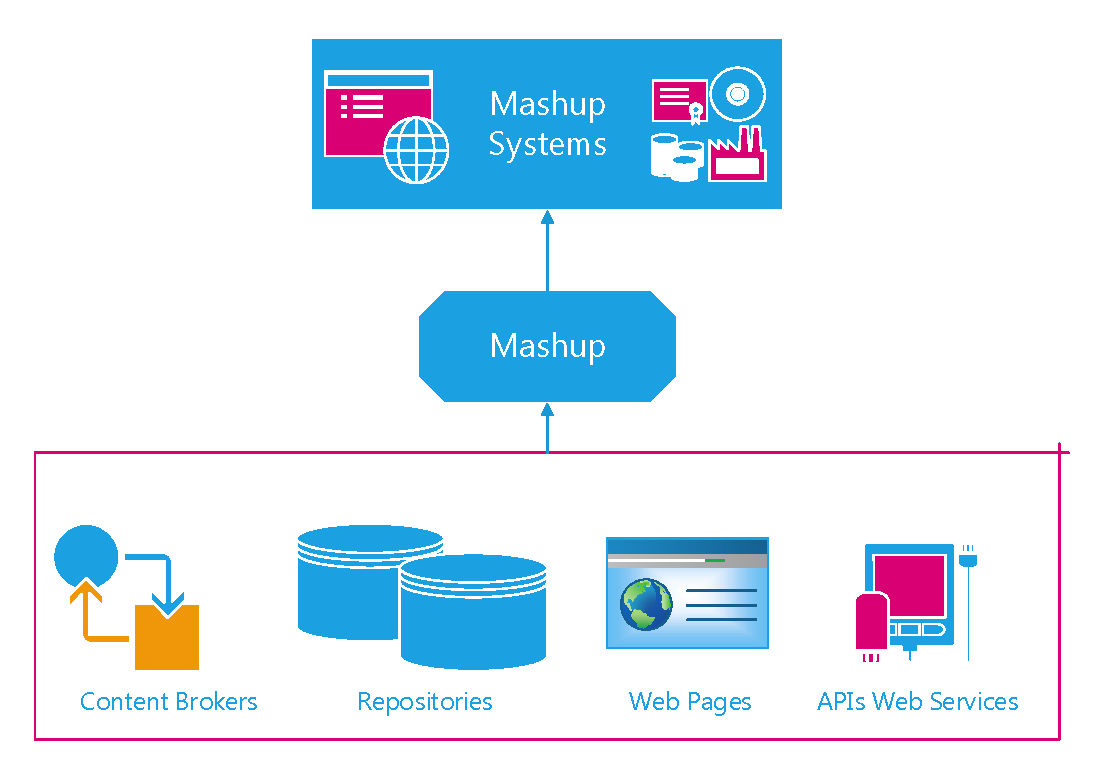
\includegraphics[scale=0.8]{chapter2/mashup}
\caption{Mashup Data Sources }
\end{figure}


\begin{itemize}
\item Rich Site Summary (RSS) or Atom Syndication Format (Atom)
\subsubitem Request is HTTP GET/POST
\subsubitem Response is XML in RSS or Atom Syndication Format.
\item HTML
\subitem Request is HTTP GET/POST
\subitem Response is HTML
\item RESTful web services
\subitem Request is typically HTTP GET/POST
\subitem Response is typically XML or JSON
\item Simple Object Access Protocol (SOAP) web services
\subitem Request is HTTP POST, XML encoded as per the description language
\subitem Response is XML encoded as per the description language.
\end{itemize}

\subsubsection{Enterprise Mashup}

Enterprise based mashups combine business-related heterogeneous data and applications from a myriad of sources (typically a mix of internal data and applications with the externally sourced data, SaaS and web content) to create a full and integrated experience \cite{hoyer2008market}. The general popularity of mashups for both business and consumers has increased in the recent years, particularly with the advent of Web 2.0 and the mass adoption of mobile technologies. Though the early mashups were heavily consumer based, it was quickly and easily determined how to create enterprise mashups to ease the consolidation of functionality onto one page that is usually found across many. This  offers serious benefits and real business opportunities for companies of all shapes and sizes anywhere in the world \cite{he2014enhancing}.

Enterprise mashups can typically be divided into 3 segments:
\begin{itemize}
\item  A presentation layer mashup presents content from various remote sources together in one unified view.
\item  A data mashup which combines, manipulates and ties together disparate data sources and presents in a single unified view. 
\item  Process mashup, which enables the users not just to mashup data sources, but also business processes, allowing customisation of process design and invoking business logic across multiple applications. 
\end{itemize}

As the techniques for creating such mashups have grown and matured, more and more companies are building business models around mashups. To capture a major share in this quickly evolving market, enterprises, software vendors and solution providers need to move quickly, and develop the mashup strategy which incorporates an entire ecosystem of data and mashup technology.


\subsubsection{Client Side Mashup}

Mashups are inherently designed in two different architectures, depending on where the processing and data integration takes place in the system. If this is the case then once the final result has been produced on the server, it is pushed to the client side for visualisation. Alternatively, both the integration and visualisation tasks can take place in the clients browser - resulting in a client-side mashup instead \cite{yu2008understanding}. The client side architecture has significant disadvantages (less security, less reliability and poorer performance to name a few) it still provides a faster user experience- with significantly less load on the servers side and much easier development. To do this, multithreading is required. This is the technique has been used by desktop and server based applications alike to help increase performance levels while performing on concurrent long running tasks \cite{patel2015novel}. 

The developers can now take advantage of multithreading JavaScript support within browsers (HTML5 introduced this feature as the Web Worker API). In later instalments, will go into more detail on this feature, and how it can be used in efficient client side mashup development focusing on process integration (PI), data integration (DI) and data representation (DR). The mashup usually refers to music or vocal editing and it is a single composition created from different songs, however data or web mashups, in a similar spirit, originated from the re-use of existing data sources or web applications, the emphasis being on graphical user interfaces and programming-less specifications. As described in \cite{eick1999visualizing}, the concept of mashups originated from the understanding that the number of applications available on the Web and the needs to combine to meet user requirements. A mashup application can be characterised as a lightweight and tactical presentation layer that uses the web platform – Web-Oriented Architecture (WOA)  - in order to integrate multi-sourced applications mashup offering. Figure 2.4 highlights basic mashup application architecture. The mashup data could be retrieved from several sources, i.e. from local databases or data sets or from external repositories, from a website, via crawling, or via a service oriented approach (SOA) through APIs and from other intermediate content brokers \cite{naik2015framework}. 

\begin{figure}[H]
\centering
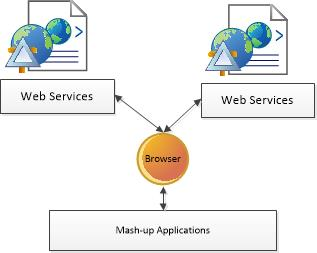
\includegraphics{chapter2/browser_mashup}
\caption{Browser Based Mashup }
\end{figure}

\subsubsection{Server Based Mashup}

The server based mashup application is widely used mashup architecture as there are more benefits and advantages. A server based mashup process, formats and compiles data at a remote site while only transmitting the output of the mashup application. Data can be re-used and high security levels are one of the key advantages of such architecture while requires trust and proxy mashup service resources for computation. Figure 2.5  demonstrate server based mashup application \cite{chen2014development}.


\begin{figure}[H]
\centering
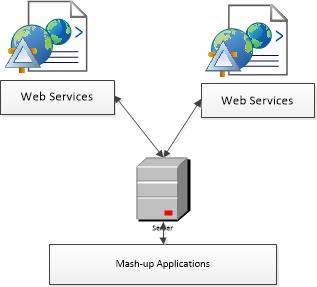
\includegraphics{chapter2/server_baed_mashup}
\caption{Server Based Mashup}
\end{figure}

\subsubsection{Various Mashup Types}

The mashup applications could be categorised into several types; these classifications vary from usage to application development - in all these mashup applications one thing in particular is very important, that is data, and, of course, data is the heart-beat of any mashup application \cite{zhao2011mashup}. The data mashup applications combine similar types of media and information sources into a single representation, or output. All the mashup applications which focus on similar types of data are categorised in this type, a good example could be a news mashup application as the application collects news, stories from different news websites such as, BBC, NY Times and present collected information in one package \cite{li2013customized}. The consumer mashup applications combine different data types, also combines data from different data sources and present application in an integrated view, there are several types of application developed to serve consumers and most commonly cited is housingmaps.com which combines Google maps data with Craigslist housing data in one integrated view \cite{zhao2011mashup}. 

The enterprise mashup applications are slightly different from data mashup, and consumer mashups, as enterprise mashups mostly combine own resources, applications and data with external web services which establishes a collaborative approach among business and developers \cite{liu2011composing}. The above are widely used mashup types however, this list is dynamic and more categories are introduced with time. Client mashups are widely regarded as solving personal situational problems while enterprise mashups focus on collaborative and coordinated problems, consumer and business mashups are used as analogous terms for client mashups and enterprise mashups respectively. The classifications of various mashup systems are highlighted in Table 2.1 \cite{11}.

\begin{table}[h!]
\centering
 \begin{tabular}{||c | c ||} 
 \hline
 \textbf{Client Mashups} & \textbf{Enterprise Mashups}  \\ [0.5ex] 
 \hline\hline
Consumer  & 	Business mashups\\
Front-end  &	Back-end mashups\\
Web Page Customisation &	Process \\
Horizontal  & 	Vertical \\ [1ex] 
 \hline
 \end{tabular}
 \caption{Classification of Mashup Systems}

\end{table}

Web page customisation mashups are more interface oriented mashup systems which helps the presentation layout of web application development; a good example is the BBC website where user can drag content boxes to see stories that are important. Process mashup helps in computation elements of application for example, data aggregations and sequential process automation \cite{de2009process}. Front-end mashup application helps in improving front-end by adding/deleting website widgets and gadgets; a good example of this type is iGoogle and Netvibes. Back-end mashup applications combines web accessible data and services into more useful web services that can be accessed easily for further re-use such as Kapow and Yahoo Pipes \cite{pipes}. Horizontal mashup applications are dependent on execution of a previous service within the application in order to represent the information, for example on a travel website, the web application needs to execute and list all destinations and then to be displayed on a map as a kind of horizontal mashup application \cite{zhao2012design}. Vertical applications depended on application output rather than execution as the next part of the application then process further information as instructions received, and the application does not provide information by itself \cite{zhao2012design}. Various types and architecture of these mashup and its benefits are discussed and explained above; combination of client side and server side mashup technologies will be utilised in our model development phase.

\section{Web 2.0}

Web 2.0 was first introduced during a conference between O'Reilly and Media Live \cite{o2009web}, and joins a new generation of web application, and represents both a practice and a technology benchmark. It has improved on its predecessor Web 1.0 in a multitude of ways, and has become more interactive and dynamic than ever before. This new improved application allows users to both access content from a website, and contribute to it - allowing to keep up with the site's latest content even if it doesn't have the latest web page version. It has also been improved for developers, allowing users to create new web applications that draw on data, information or services that are available on the internet. A more comprehensive list of differences between Web 1.0 and Web 2.0 technologies are undertaken by Cormode et al \cite{cormode2008key}. 

This new technology is focused on the reuse and open standard based technologies with both scalability and flexibility in new dynamic environments. Web 2.0 technologies can not only help with the creation of standard web application, but it can also aid in the construction of circumstantial applications, which can explore enterprise applications and data for business users and customers. It can help limit the possibility of information  overload while adding a new dimension of modernisations for businesses and end users. It has improved on various other aspects of Web 1.0, including commercial impact, the re-usability of applications and data, and even user friendliness. These new technologies are developed and positioned on uncomplicated programming imitations, and these can help rapidly accelerate its time to market, and improve the usability of enterprise assets \cite{21}. From the conference, O'Reilly Media have given seven principles, and fulfilling these will qualify a company or application to be categorised as a Web 2.0 application. The success of the Web 2.0 application will be judged on these principles \cite{webtim}: 

\begin{itemize}
\item Services, not packages software with cost-effective scalability
\item Control over unique, hard to recreate data sources that get richer as more people use
\item Trusting users as co-developers
\item Harnessing collective intelligence
\item  Leveraging the long tail through customer self-service
\item Software above the level of a single device
\item Lightweight user interfaces, development and business models.  
\end{itemize}


The core of the Web 2.0 application is to encourage an individual's freedom, not only to create, but to annotate, comment upon, index and share the content within it - completely bypassing the more traditional models of editorial control, centralised publishing and professional indexing. The flow of content is now no longer a strictly top down operation, now flowing from classic producers to consumers. The traditional distinction between the content producers and the consumers is blurred, and a new bottom up movement ban be instigated, one which facilitates self-organisation. Once ordinary users get more involved in the process of content creation, self-organising communities emerge. To support this, only need to look at Wikipedia - which builds on the tight involvement of users, sense of community and deep dedication to developing a large and unprecedented knowledge repository. The same responses to other community driven websites, such as blogs, wikis and podcasts, and in all of these the sum of community knowledge is larger than that of the individuals. This harnessing of collective intelligence is an essential part of the Web 2.0 application, with the intention of turning the internet into a form of global brain. While anyone on the internet can edit the existing pages of wikis and add new pages at any time, more scientific articles found in Wikipedia are fully comparable with the corresponding information from sources such as the Encyclopedia Britannica in terms of accuracy \cite{berthon2012marketing}.

\subsection{Web 2.0 Models}

The beauty of Web 2.0 applications are embedded in real business models \cite{webtim}. For example, the fact that Google has recently expanded dramatically and the credit largely goes to the search and advertisement market, which has the highest growth potential on the internet \cite{21}. Because of its success and versatility, a great number of studies have contributed to many Internet business models. It is because of this that Afuah and Tucci \cite{22} defined two classifications of business models. The first classification is adopted from \cite{23} and was based on the differences between traditional and Internet business. This included elements such as e-shopping, e-procurement, e-auction, e-mail and information brokering. 

The second classification was initially constructed by \cite{24}, and this mainly presented the taxonomy of the various categories of business models, including brokerage, advertising, informatory, merchant, manufacturer, affiliate, community, subscription and utility. But this itself has caused issues, as there is rarely a categorisation of Web 2.0 business applications based on the value, it can generate for both the customers and the service providers. Based on both user involvement, service provider efforts and the various sources of revenue, the following factors to act as differentiators between the different types of Web 2.0 business models. This measures the degree of consumer participation in the design, development, storage and reuse of the systems and application on the Web 2.0 horizon. The learning management system (or LM for short) is designed to raise learning management activities while promoting the acquiring of data, transfer of data and sharing of the content and information. Internet based businesses may already support users with some forms of learning management participation, such as free exertion of knowledge management and the regulated processes of authenticating the correctness of data. This syndrome the rationalised processing of the knowledge network and learning commerce, and even knowledge capture technology such as relationship recognition between new and previous content \cite{sclater2008web}.

As an example, Wikipedia is a huge encyclopedia which was collectively created by many of its users from across the world, and offers a recognised process for users to add and edit knowledge on the Internet. Any user signed up can log in, edit and offer corrections on any published article, and because of this the content of Wikipedia is being constantly monitored and improved. It is logged at making thousands of changes an hour, all of which are recorded in article histories. Any inappropriate uploads or changes are quickly moderated and removed, and repeat offenders can be blocked from changing articles in the future. Users can also add hyperlinks for readers reference, and all articles are arranged in proper categories for ease of reference. All articles that are arranged this way benefit from the search function to allow readers to find information easily \cite{aghaei2012evolution}. Businesses often price applications or commodity depending on cumulative sum of the cost of assets, crude elements and labour for generating the objects. A Web 2.0 user will consume large sums of resources in the applications, internet bandwidth, research and development and knowledge generation \cite{shang2011understanding}.

\subsection{Web 2.0 Usage}

With the creation of Wikipedia, the internet fast became home to a revolutionary website; a free, online encyclopedia backed by an expert team comprised of writers editors and proofreaders. But in the early days the results received were poor at best, and the team had to devise a new concept in which readers are allowed to self-select what roles they wished to play, what content to create and what the content was. This change resulted in a group of people who were extremely enthusiastic about the project and had a vested interest in the quality of the output, and this brought the quality of the online encyclopedia to the surface and revealed its true potential. This success triggered a phenomenal outbreak of social encyclopedias, Facebook, Flickr and Youtube, and this industry is still growing. At the heart of these new web-based solutions to find a web of social network services, spawned with the idea of building more of these online communities with people who share interests and activities, or wish to explore the interests and activities of others \cite{kamel2007emerging}. Web 2.0 is yet another new revolution in the direction of the computer industry and solutions for businesses. This was caused by the movement of company intelligence and the management of business ideas, with the internet as its new platform. In an attempt to understand the rules for success on this new platform, a set of experiments were applied to a heterogeneous mixture of relatively familiar emerging technologies, all based around the idea of harnessing the collective intelligence of crowds to give information new value \cite{webtim}. 

This new idea about the creation and collaboration of the collective intelligence when placed into a database sitting behind the internet technologies is crucial for the success of the complex group of different solutions known as Web 2.0. It is safe to say that Web 2.0 is a completely open concept, which does not have any hard boundaries, but instead has a gravitational core. A simple set of principles and practices tie together within the internet as a platform for the solutions. The term Web 2.0 refers to the cumulative changes in the ways multiple software developers and end-users alike use the internet. It refers to an attempt to conceptualise the exact significance of a set of outcomes that are enabled by these internet technologies \cite{boateng2014web}. The industry standard technology used for Web 2.0 is Asynchronous JavaScript and XML (AJAX). This is a method that allows a minimal data exchange with the back room servers, and allows a group of interconnected web development techniques to be used on the client side to create interactive and responsive web applications or rich internet applications. Because this system has a dynamic and immediate update of the pages content in the background, without interfering with the displays of the existing live page \cite{webtim}. Whilst a good tool can facilitate work and help in the ease of doing a job, it does not provide new solutions to problems or innovative ways to work. Web 2.0 facilitate users with content creation and service availability - with the advantage of a collective intelligence strongly based on mutual trust but driven by common goals and motivations. Maintaining the content of the internet in this new way breaks away from the traditional page metaphor, and instead relies on the composition of microcontents. Using this technology user can define a whole new set of content building blocks, where blogs are about posts and not pages, and wikis are transformed into endless streams of conversations, revision, amendments and truncation. Podcasts will be shuttled between websites, while RSS feeds diversify players. Once created, these AJAX technology based content blocks can be saved, summarised, addressed, copied, quoted and even built into new projects. This creates a whole new content metaphor, and one that is rising on this original microcontent drive. This allows users to develop the contents completely collaboratively and open it to the world, and it is this openness that is essential to the whole concept \cite{mesbah2012crawling}. 

Web 2.0 concepts are microcontent and openness, but these two elements are only part of a larger strand of concept. Web 2.0 brings out a whole new role for users, putting more of a foundational role on the old wisdom of the crowds argument. This new platform responds to its users in a completely new form of metadata affectionately known as folksonomy - organised on the sets of words generated by the users and attached to the contents of the web \cite{chen2014retracted}. There are a few problems with the idea of wisdom of the crowds, and one of the most prominent of these is the value of the data produced by multiple sources that are so out of any form of control. Web 2.0 gives every user the opportunity to take part in the creation of the massive log of contents in the back end database. The content created is unstructured with dubious accuracy, and this leads to huge and well known problems in the field of knowledge management. However there are a few different approaches to solve these problems. For example in blogs, user can see that the microcontent is signed, albeit usually under a pseudonym, but the author who uses this sign takes full responsibility for the microcontent. The same theory applies to pictures uploaded to Flickr. More of a problem is presented with networks such as YouTube, where on average 100 hours of video is uploaded every minute and it is not possible to organise and review the content \cite{youtube}. This instead puts the entire responsibility with the authors, as is also the case on social networking platforms like Facebook, MySpace and Twitter. In handling content on these platforms, a whole new set of tools and techniques introduced for the creation of wikis, blogs, tagging and feeds, which automatically helps other participants in a network to share links and ideas \cite{auer2007dbpedia}.

\subsection{Enterprise 2.0 - An Overview}

Enterprise 2.0 was a concept first introduced by McAfee in order to showcase how Web 2.0 technologies can be used within enterprises. The focus was to explain how Web 2.0 could make practices and the efforts of knowledge workers more visible. This is in reaction to the initial response to Web 2.0 by the businesses - when introduced it fascinated almost everyone, but it did not seem to register with enterprises. In order to take these (or any) emerging technologies seriously, companies needed to see real case studies of the use of Web 2.0. Case studies in which the application had been studied and analysed from multiple perspectives, including security, consistency or scalability. Enterprise 2.0 need a set of best practice descriptions for its use, and specific guidelines on Web 2.0 technologies within organisation \cite{mcafee2006enterprise}. How was the new technology of Enterprise 2.0 studied and discussed in other areas? While there have not been many in depth qualitative analysis on Enterprise 2.0 within the work context and its impact, there have been multiple studies on the direction, detail, quality and format of social networking systems (particularly Facebook and Twitter). There are even qualitative studies focused on application and real use within business. However in recent years, some managerial journals have published new results of the applied Enterprise 2.0 technology, and some books have even been published with a specific emphasis on providing explanatory guidelines for management in enterprise. While these sources were a considerable jump forward, it does not exhaustively and qualitatively describe how and in which areas this new technology is more efficient for enterprises - or the additional value it can have to cooperative work. This is something that the research literature still lacks - an in depth analysis and explanation of cooperation processes in very complex development environments. This is the sort of thing that needs investigating, by basing the analysis on central concepts such as awareness, trust, openness, sharing through data mashup tools and information visualisation \cite{mcafee2013enterprise}.

However, introducing changes into any organisation is a difficult subject as resistance to change is often immediate and dramatic, without any deeper thought. Organisational culture also impacts the attitudes towards Enterprise 2.0 adoption, because the organisations general attitudes towards collaboration, open communication and information sharing hugely affect the acceptance of Enterprise 2.0 by employees and managers. The common fear the organisations have is that it will lose governance over information, and Web 2.0 tools as perceived as a potential risk, particularly in the field of data loss. This is viewed as a direct result of employees sharing information on blogs or social networking sites. There is also a huge concern for decreased employee productivity, or the possibility that the wrong information will be posted on a network by an employee, or even that employees will write questionable or offensive materials on a network. These fears are what fuels the standardisation of office policies and processes when it comes to social networking and collaborative work - usually opposed. This is particularly true for organisations who operate under a command and control culture \cite{williams2013enterprise}. Despite all of these barriers, some organisations are not only starting to use Web 2.0 technology, but are also leveraging it to change management practice and organisational structures. Those organisations that have recognised the innovations that Web 2.0 technology represented by innovation instead of price have tapped into a priceless idea - using the knowledge (and tacit knowledge) of workforce and therefore encouraging collaboration among knowledge workers using the Enterprise 2.0 tools. Many more organisations are starting to see Enterprise 2.0 technologies as an opportunity to increase company's revenue and margins, and see its many benefits. The undeniable fact is that Enterprise 2.0 is an unavoidable technology - one which is becoming increasingly popular among enterprise specific users, and more so among knowledge workers and digital natives who have grown up with the web \cite{kim2013building}. 

In these modern times the nature of work is constantly evolving, and being driven by the Web 2.0 technologies that enable and enhance social activities it has quickly taken on a significant role in the workplace. Enterprise 2.0 has not only become a competitive necessity, now organisations must be ready to use the technology that supports it. After all, simply adopting the technology in a process does not necessarily improve the process by itself. The technology must be fully assimilated into the organisation in order to gain the full competitive advantage and considerations about technological capabilities, willingness of adoption and organisational size must all be taken into consideration, helping in the evaluation of the organisations readiness for Enterprise 2.0 \cite{mcafee2009enterprise}.

\section{Data Storage}

Data warehouses can be characterised in a number of different ways, but for now with a very basic principle. A data warehouse is made up of a complex architecture including data sources, data staging areas, operational data stores, some global data warehouses and even client data marts and this makes an incredibly complex thing to modify \cite{berg2004qualitative}. A new business process is often the catalyst for change within the data warehouse and these changes trigger the need for new software. The warehouse is then used to define the requirements for those software systems so it can be designed to co-exist or integrate. There have been many hundreds of hours spent researching and working on the industry, but addressing the delicate alignment between business processes and information technology has only been mentioned in passing \cite{rabl2012solving}. Instead the majority of software developers are continuing in ignorance of the business processes required or unable to read the models provided (this is not surprising, as different modeling languages all use different diagrams and notations, and are all used in both domains). Instead of letting this continue. The solution here is to fulfil the needs of developers and the business users by applying more business-oriented approaches to the development of a new data analysis solution.

Most of the existing visualisation systems \cite{fry,north2000snap,spotfire,tableau} are focused on the visualisation aspects of the data while limited attention is given to re-use of the visualised content. The beauty of the modern applications are the re-use of the data elements. There is a knowledge gap as how could we utilised and re-use visualised content generated by visualisation tools.

\section{Summary}

Existing techniques and technologies in acquisition and data analysis are discussed in the first part of the chapter. Web and data mining techniques are further discussed with more insights to the mining procedures adapted in the mashup and Web 2.0 scenarios. Existing models, systems and frameworks utilised in information visualisation are highlight from various angles. How existing tools are going to be linked with the proposed model. Key elements of the proposed research such as multi-coordinate visualisation and multi-attribute visualisation techniques are explored. The importance of Web 2.0 demonstrated along with various references to the current proceedings. Web 2.0 facilitation of the proposed model put forward. The mashup technologies are discussed in detail with various types of mashup architectures available for application development. 

Every company that understands business transactions is closer to understanding clients and their needs; which is one step closer to being able to meet and exceed \cite{price2011best}. And after all, happy customers leads to happy businesses \cite{plassmann2007companies}. That's why the next chapter will propose a compound information visualisation model which will help in answering most of the data problems. A comprehensive four step visualisation model is proposed in the next chapter. 

% Chapter 3

\chapter{Research Methodology} % Main chapter title

\label{Chapter3} % For referencing the chapter elsewhere, use \ref{Chapter1} 

\lhead{Chapter 3. \emph{Research Methodology}} % This is for the header on each page - perhaps a shortened title

%----------------------------------------------------------------------------------------

\section{Introduction}

The proposed information visualisation model is discussed and substantiated through design flow charts. In the first part of the chapter, a brief introduction to existing information visualisation model along with the proposed model is highlighted. The research model presented in this chapter is further explained with extracted code sample from the application developed for proposed visualisation model in the next chapter. The proposed visualisation model is validated through three experiments. The next two chapters are based on different experiments while further experimentation and comparative analysis discussed in chapter 7.

\section{Seven Stages of Data Visualisation}

The process of understanding data begins with a set of numbers and a goal of answering a question about the data. The steps along this path can be described as follows \cite{fry}:

\begin{enumerate}
\item Acquire - obtaining data from local, remote sources through web services or direct data set access.
\item Parse - organising and giving structure to collected data in the system environment. 
\item Filter - removing all but the data of interest.
\item Mine - the application of methods from statistics or data mining, as a way to discern patterns or place the data in mathematical context.
\item Represent - determination of a simple representation, whether the data takes one of many shapes such as a bar graph, list, or tree graphs.
\item Refine - improvements to the basic representation to make it clearer and more visually engaging.
\item Interact - the addition of methods for manipulating the data or controlling what features are visible.
\end{enumerate}

\begin{figure}[H]
\centering
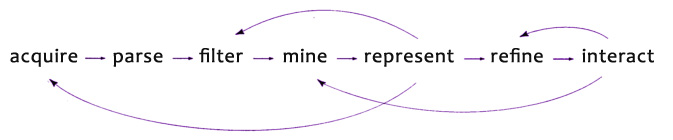
\includegraphics[scale=0.6]{chapter3/J_Fry_V}
\caption{Fry's Visualisation Model \cite{fry}.}
\end{figure} 

The research model shown in Figure 3.1 will be adapted for data visualisation which is a complete data visualisation process but the focus will remain on important elements of visualisation process and adjustment to process and development of the model to meet the requirements of small to medium size businesses and individuals with easy to use system approach. The research model is explained in the following section.

\section{Proposed 4 Stages of Visualisation}

The proposed 4 stages of information visualisation model is a complete set of action which could be applied to any kind of data set for data analysis and exploration purposes as presented in Figure 3.2.  

\begin{figure}[H]
\centering
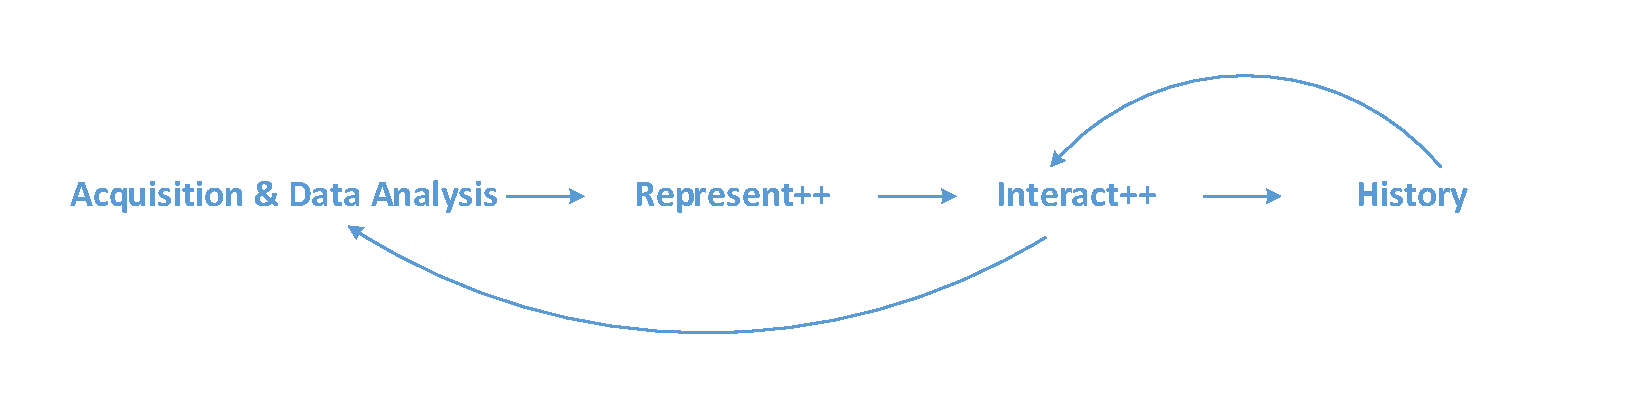
\includegraphics[scale=0.59]{chapter3/model}
\caption{Proposed Visualisation Model}
\end{figure} 

The first step of the information visualisation model proposed in this research is acquisition and data analysis. This part explains how complex raw data sets are converted into a normalised and easily retrievable data structure which is then passed onto the data representation layer. The data representation layer processes retrieved data from the database into visualised forms requested by the user or requests initiated by the predefined instructions by web intelligent agents. The data representation or represent++ layer pushes processed visualised data on to the interact++ layer where user and the computer system or application interaction take place with the end user. The users at the interact++ layer could request further analysis of the data and thus instructions are sent to the acquisition and data analysis layer to re-process information for more insights about data processed in any given data set. The acquisition and analysis model re-sends requested information to data representation and exposed to users at the interact++ layer. History layer where stored or exported reports are processed. The information could be requested by the users at the interact++ layer and made available upon demand. This layer is very important as re-using system generated particulars in the past and thus making this layer extremely important for version history control or comparison purposes.\\

Transactions tagging and linked data visualisation along with multi-coordinate and multi-attribute visualisation techniques and approaches were absent in the existing tools and models. Similarly, robust and effective solutions to export and store visualised content was not available in the existing tools. Acquiring and processing complex and diverse data elements. Visualising complex data elements into simplest of forms, thus making it very easy for the users to analyse data more effectively without any prior knowledge of the visualised content. The concept of this research revolves around information visualisation through mashup application for enterprise practice to understand huge transactional data for resource and decision making purposes, focus is on understanding data through visualisation, interactivity of the system with end user, storage of generated results for re-use and comparisons purposes and finally light weight mashup applications - resource friendly and economical. All the four stages of the visualisation proposed in the visualisation model above are further explained in more detail below.

\subsection{Acquisition and Data Analysis}

Data is a term, that's thrown around a lot in modern business circles. The problem is, it's such a wide term that it can sometimes be difficult to define. To clarify - data can be any kind of fact, figure or textually based data that can be analysed and processed using computers \cite{chamberlin1976sequel}. Because of the recent surge in data analysis, the processing power and storage capacity of modern computers has been hugely affected - and this has played a vital role in further data growth. There are many types of data stored in computers and vaults today. For example, transactional data, as the name suggests, this refers to data acquired during transactions. This can include sales, purchase or even cost and accounting data, and this often relates to the business operations side of things \cite{abadi2009data}. Some could be categorised into non-transactional data type, this data is found outside of direct business statistics - and is instead more about industry forecasts and economic data \cite{herlihy1993transactional}. Finally, meta data is how it is defined and what class of data each segment belongs in, and contains information on the data, including how it is structured and defined and where it came from \cite{harris2009research}.
\end{itemize}

Data analysis plays an important part in understanding complex data. By going through the computational data analysis and representation process, chunks of data that were meaningless can now be presented in an easy to understand and clear way. The different approaches to understanding data and how it is typically retrieved from various data sources for analysis will be discussed. The most important factor in data analysis is that it leads to information. This information is essential to understanding business and identifying patterns, allowing us to hone business models to work at their highest efficiency. To combine the understanding of data with the analysis of patterns, associations or other relationships, and the information is a very powerful tool. It will be useful to understand, for example, how many sales a single staff member converts in one month, which can help in streamlining the performance of the sales team. Data harvested by the system on a certain staff member can be analysed, and can produce a figure, giving an answer to the question raised regarding business sales \cite{hair2006multivariate}. The information gained can then be used to discover new patterns and trends - letting users to explore possibilities and predict outcomes before taking the risks. For example - users can use data analysis and information to find out how good a certain staff member is at converting sales, which of the sales force has the lowest conversion rate and who has the highest, and all of this can lead to a greater understanding of sales force, with facts and figures to  evidence it \cite{larose2014discovering}. Most of the data that will be processed in this research using modern computational data processing and analysis techniques which has been harvested in a readable format. Disks are one of the most common ways to store large or small volumes of data, and is easy to source and interpret. Data is simply removed from the disk and processed by data analysis web intelligence agents, with little computer involvement at this stage. This is because the data stored on disks is already in a human readable presentation format such as PDFs or JPEGs, and is easy to decipher and interpret without added help.  

A more modern addition to the acquisition of data is from network streams  - a technique made possible by the Web 2.0 era. One of the most common examples of data acquisition from networks is usually through network streaming - particularly data feeds generated by rich data sources. This can be anything from a news feed generated by a news website to a product and transaction feed from a retailer. However the downside lies in the huge variability in network streaming - there is no consistent format for the data, and it can vary not only from source to source, but within the same source. Luckily there are some commonly used themes that makes it easier for the data acquisition agents to retrieve the information required from such sources in a way to understand and interpret \cite{nandy2014real}. A database is a much easier source to collect data from, simply because a database by nature is a collection of data in organised and formatted structure. Because the data is so structural it can be easily retrieved and analysed when required \cite{urban2014integrated}. The majority of databases are made up of tables, and require a set of connections to enable data streaming - and these can be made using database drivers. As an example, a table within a database could be titled student. This table will hold all of the student data - including name, address, phone numbers etc. This data would lie dormant until it is retrieved via a query. Queries are usually a command or instruction made in SQL (Structured Query Language) and issued to the database. An example would be:

\begin{listing}
SELECT student_name from student WHERE name is smith;
\end{listing}

This query would produce rows of data that match the search criteria (i.e. where the students name is smith). While the above is a very basic query, it is the general way in which the information is retrieved from databases - by sending instructions to the required data. For large databases with a huge volume of data, more complex queries can be manipulated to gather the right data. The only major drawback in acquiring and processing information from databases is the retrieval process. Databases work on an information pull and push concepts (where information is only dispensed when a command is issued of a certain event occurs), and this limits the amount of data one can access in a effectively. As the data is only retrieved when specific queries are issued, it is not always available for large volume processing and analysis, and one must follow this push and pull structure for every element, and every different type of information required.

The acquisition of data has itself become a vital part of the information processing practice, and systems are being developed that will know the relevant attributes needed and make it available for processing. For example, if the system only needed to know the name and address of a student, it could ignore all other fields as are not required for that particular search. The data acquisition can vary depending on data source and methodology, our computational data analysis and representation model can acquire the majority of data from both relational databases and different data feeds in order to validate the visualisation model. Data parsing is the technical term for splitting a large data set into much smaller sections through defining criteria before structuring and organising it. This process makes it much easier for automated systems to interpret, manage and transmit the data. Any data could be acquired through the parsing method which can then be structured and organised in multiple ways to allow data to fit into a certain system environment. Data sets usually consist of various large data elements, it's not always feasible to process all of it. Often there will be elements of the data sets that are not required or completely irrelevant to the analysis being done. The proposed system only allows the relevant sub-sets of data to be retrieved, and those that don't meet the conditions or criteria are not harvested in the first place. For example, instead of retrieving all the rows of data from the student table, the user or even the system can set parameters and condition criteria to help filter down the elements required before fetching  from the system. The filtering is the process of removing unwanted or un-usable information from the data sets. Closely related to user input, the systems will refine the data sets when requested , to ignore information that does not fall within the specifications, or that is irrelevant or repetitive. While some data is removed from the data sets before these are processed for representation - it can only be done if there is user defined conditions put in place by web intelligence agents in the pre-defined data filtering stage. Data filtering could have a secondary use. It can be used to restrict access to sensitive information within databases - allowing parameters to be set that restrict user access to certain information such as credit card numbers, social security numbers and in some cases personal information. This makes data filtering the perfect solution for managers and directors who are wanting to hide such sensitive data, and avoid an ordinary staff member stumbling across it.
 
Larger data sets can sometimes prove challenging to analyse, but often mined for a number of different things - such as a deeper understanding of data categorisation which can help improve the analysis. There are many different kinds of categorisation, but may have different names tend to be for the same purpose, and can be summarised as follows:

\begin{itemize}
\item Grouping Data: Data can be grouped together to help explore patterns and analyse the data sets in more detail. How many bookings staff convert in a single day? Finding the two aspects of date and conversion rate and combining it will provide the answer. Data is stored or extracted into a more logical pattern to further explore the data relationships. For example - what percentage of conversion does a staff member of a particular organisation do in a single month. To answer this question, one need to examine how much that staff member contributes to all the sales in the company, and explore in detail the relationship between sales transaction and each staff members conversion rate \cite{hedges2014statistical}.

\item Data Relationships: This refers to exploring the relationship between various data elements to allow us to find any association or relationship. This could be used to find out why the conversion rate falls when a staff member reaches their target \cite{vidulin2014combining}.

\item Data Patterns: Data can be mined to explore different patterns of behaviour within data. This could be used to discover why the conversion rate is always at its highest when staff members haven't reached their targets \cite{singh2013web}.

There are many elements of data mining that relate and mix with each other, there are a few data mining principles that always hold true:
\begin{itemize}
\item Scraping or extracting information from a data set onto a particular segment
\item Stocking and maintaining information in multidimensional data sets
\item Connecting analytic systems and data sets
\item Making data available in a useful form
\end{itemize}
\end{itemize}

It should be fairly clear that data analysis is all about collecting statistical data and analysing it to predict behaviours, identify trends and explore new insights into the business. There are many techniques for data analysis, such as Single Variant (where data is analysed for a single-variable distribution) and multiple Variant (where it is analysed for multiple dimension attributes) Data Analysis, and all of these techniques can be practiced. But the main message is that the researcher using the techniques should be fully focused on the approach adopted, and be completely satisfied with the analysis process. Data visualisation is a multiple layered practice, but at the heart of it all is the structuring of data. In the proposed methodology the system will establish whether the information visualisation request that is initiated from an Enterprise 2.0 or a non-Enterprise environment. 

In an Enterprise 2.0 environment, the proposed system will already be aware of the environment and will have pre-authorised direct access to the data sets through web services and API's (Application Program Interface) or web intelligent agents. Various mashup applications will also be able to understand and interpret the data structure, also directly access and pull the relevant information for visualisation purposes. Because of this, this versatile system will already have multiple connections and entry points for the data sources in real time - and if the source should change in any way then the proposed system application will be automatically updated with data acquired from the source. The processing in a known environment (Enterprise 2.0) will facilitate the first four steps (acquire, parse, filter and mine) through API's and web services or through web intelligent agents(PHP predefined functions). For example, if the application now requires sales figures, various mashup systems and web intelligent agents could log in and access the sales figures parameter through API's. This data would be drawn out in XML format or SQL Queries and be passed straight to the represent layer for visualisation.

If the environment is an unknown (a non-Enterprise environment) then this can make accessing data sets through API's extremely difficult as the application or the source might or might not be able to support web services or remote data retrieval. This can also mean that the data is stored in an unknown structure. In these cases, the mashup application can request data through a custom tool called visualixer, this tool has been specially created and developed for the non-enterprise data sets. The tool has the ability to read, mine, filter and parse data acquired from the importer tool and has a specialised data representation layer which visualise data and push it to the user at the interact++ layer. The visaulixer and its features are discussed in more detail in chapter 6.

\begin{figure}[H]
\centering
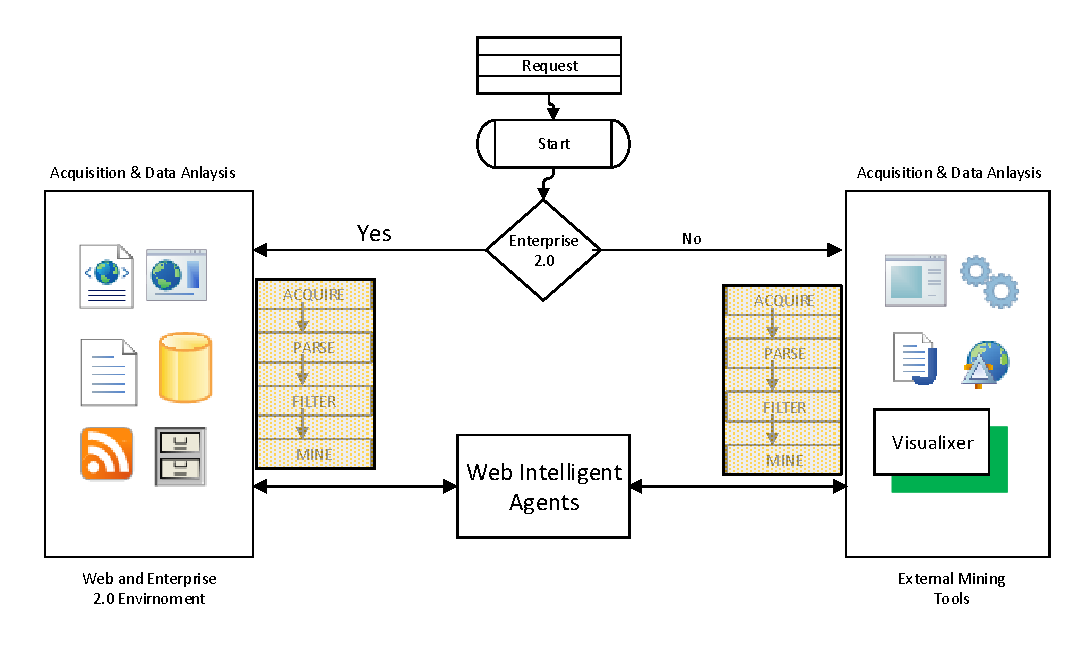
\includegraphics[scale=0.8]{chapter3/data_analysis_flow}
\caption{Data Analysis System Flow Chart}
\end{figure} 

Figure 3.3 shows the data analysis flow in the system. In Enterprise 2.0 environment where data is in a normalised or known state, information is then retrieved through web intelligent agents(PHP functions). However, if the data is not in enterprise or normalised format it is then passed onto a more detailed data analysis process for which a bespoke application is developed called visualixer which is further explained in chapter 6. 


\begin{figure}[H]
\centering
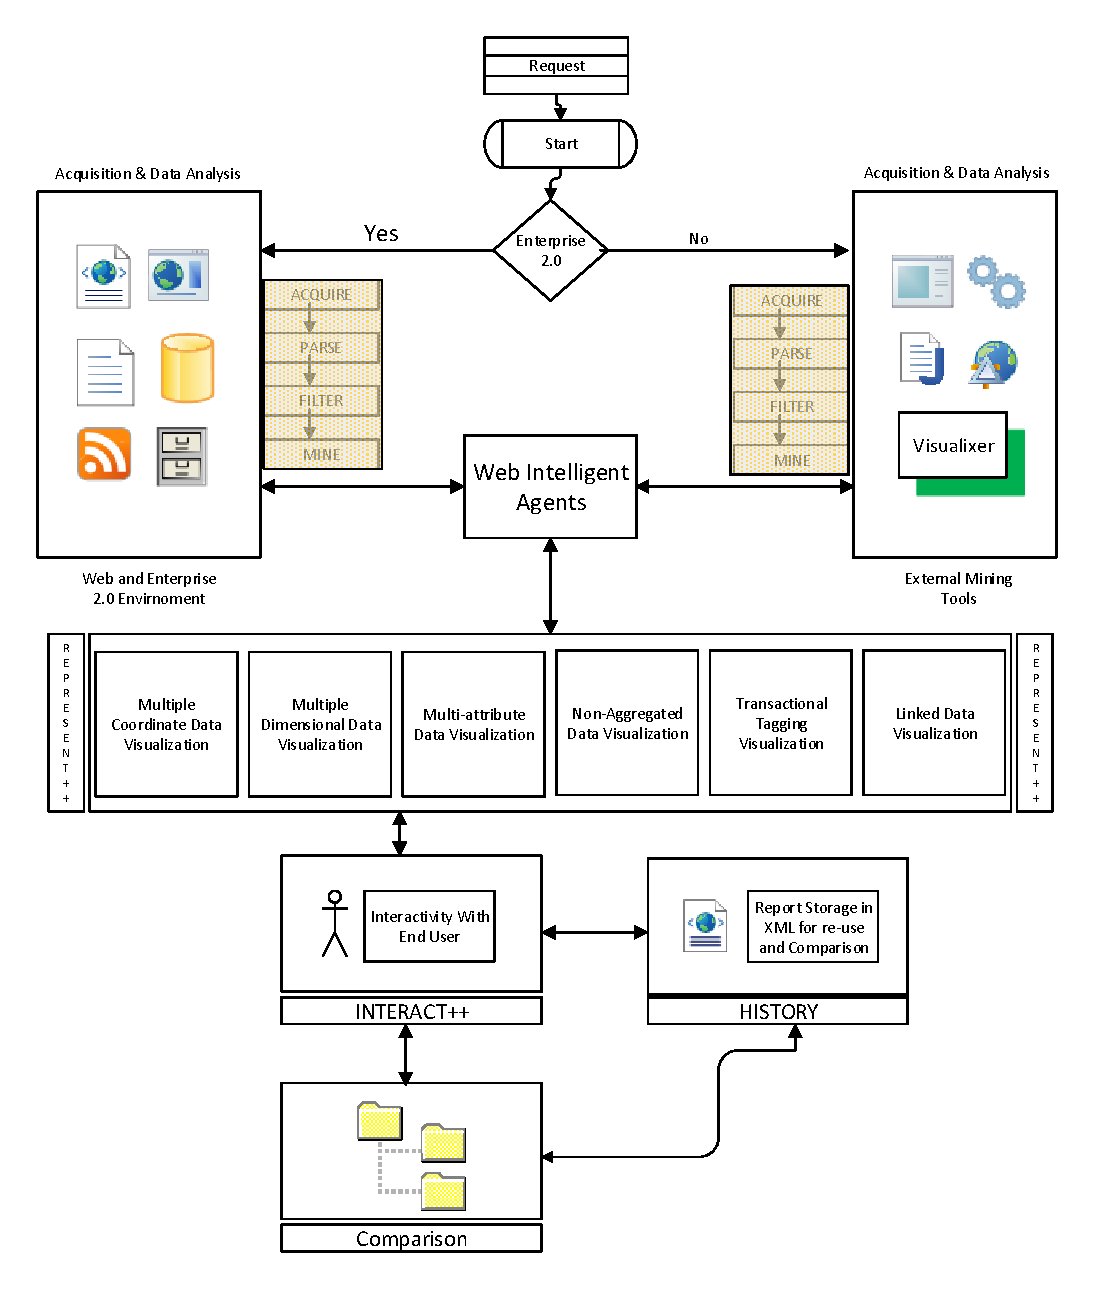
\includegraphics[scale=0.8]{chapter3/system_flow_chart_full}
\caption{Proposed Theoretical Visualisation System Flow}
\end{figure} 

The full system flow chart is presented in Figure 3.4, in the next section represent++ where data representation process is further explained in more detail below.

\subsection{Represent++}

This layer is called represent++ and it is responsible for visualising data and producing visualised content. The layer is labelled represent++ because it is different from Fry's represent layer \cite{fry}. The represent++ layer will remain mostly the same for different type of data processing and visualisation, regardless of whether the data came from an Enterprise 2.0 or non-Enterprise environment. This is incredibly useful as it has become a key step in the understanding of transactional data and non-transactional data. This layer has been contributed with new approach in processing and visualising data as this layer has been extended into more elements, for example multi-coordinate visualisation, non-aggregated data visualisation, transactional tagging visualisation and linked data visualisation.

Multi-coordinate visualisation is used at the representation layer, which allows users to put visualised data into coordinated views for ease of understanding. If one element of the visualisation updates, the other elements update automatically and refresh the visualisation for an updated view of data and information visualisation. It also means, users can visualise the elements of the data in different styles, which helps key decision makers see the data from different angles - giving a full view of the data. Introducing a multi-attribute, multiple dimension data is a representation - and this allows to analyse attributes like price, product, customer and transaction in one go, plus all attributes related to a transaction could be visualised in one place. An important feature to consider in Web 2.0 is transactional tagging. Tagging is defined as a non-hierarchical structure achieved by terming or assigning a keyword to a particular element of the data \cite{golder2006usage}. The transactional tagging is introduced in this research and this new method will help those key decision makers to gain a real insight into transactions and analyse in various different ways.\\

This could be through time, space, monetary value etc. Each transaction can be tagged manually by end users, so a company who takes online orders or sales, staff can tag each transaction for their ease and for ease of analysis. It could be tagged in any combination of words - for example corporate, school or showbiz, and our intelligent mashup application can analyse these tags, sort and visualise for different uses. These could even be given secondary tags by the analysers for better understanding of the data at a later stage - for example, a secondary tag could be markets, and when needed the data will be pulled for analysis. This approach is adoptable by web transactions, which can be automatically tagged by web intelligent agents who would categorise transactions by location, value, product type or analysis against records.\\

The represent++ layer uses charts and graph libraries to utilise and visualise the data retrieved during the data acquisition stage. To make it easier to understand, the data needs to be represented in incredibly basic forms, such as bar charts, pie charts and tree maps. These techniques might seem primitive, it can be used to answer some complex analysis questions with a very visual output. There is a huge range of visual forms to present data in order to help users select the type of data visualisation relevant to the question. This ensures that the message is clearly conveyed and understood across the board. \\

In Figure 3.4, data representation layer which is called represent++ is highlighted in the system flow. The acquisition and data analysis layer push retrieved information to the representation layer, where complex visualisation processing with the help of existing simple visualisation graphs and charts, a more defining outcome is achieved. The various kind of highly complex visualisation processes are delivered within the simple form of representation. For instance, linked data visualisation is formed by combining two or more graphs while showing relational data elements. The represented or visualised data is available to end user at the interact++ layer - where user has the ability to refine the result or request detailed analysis from the system through users interface layer. User interaction layer is further discussed in the section below.\\

\subsection{Interact++}

There are two main aspects of interaction. Data and human computer interaction, Data interaction is drilled down in refine phase where various types of processes are applied to data for making it more meaningful to systems and users \cite{hix1993developing}. In interact++ layer, the proposed system is focused on human prospective – for example layout, padding, proportional aspects, graphs interactivity, scaling and zooming aspect of graphs for improving system and data user-ability. Customisable widgets are introduced on the interactivity layer of our proposed model; at this layer a user-friendly mashup interface will be build which will be highly customised to meet personal demands and will have options to refine results for further analysis. For example, a manager would require a company overview while a team member will only be interested to see the team performance, to accommodate this requirement the drag and drop mashup widgets features are introduced \cite{wu2010widgetizing}. 

Graphs should be clearly and precisely displayed for information analysis. Padding of graph elements should be consistent to make the graphs look pretty. Proportional aspect of visual graphs should carefully be crafted to make right sense of data and information and knowledge is gained easily as it’s the sole purpose of information visualisation. Interactive graphs are getting very popular these days as information is visualised in two-way or one-way flow on the charts, system receives information from sources, these are kind of dynamic graphs; the flow of data could be based on timely based intelligent agents or chart functions visualise data as it is fetched from the data source. This type of visualisation is effective for the data which is updated in real time such as stock market data or company sales and transactions which gives overview about business state. Zooming changes the magnification of a graph without changing the size of the figure or axes. Zooming is useful to see greater detail in a small area \cite{ondov2011interactive}. 

Data interaction is handled through intelligent agents at represent++ stage, however data interaction at this level are focused on human-computer interaction. The system will decide best possible type of visualisation so that data question is easily and thoroughly investigated and answered. 

\subsection{History}

Report storage is a novel contribution to the theoretical visualisation model shown in system flow chart in Figure 3.4, system generated reports and is stored and users are enabled with the ability to export the generated reports in various formats such JPEG, GIF, PNG, PDF as that it could be re-used for analysis and comparison purposes, system will have the ability to allow internal and external requests for data reports.\\

History features in any visualisation system can play a vital role
supporting iterative analysis by enabling users to review, retrieve,
and revisit visualisation states. Moreover, history features can assist users in creating reports or presentations, enhancing communication. History features can also aid research and development. History log analysis of both individual and aggregate usage can
identify common usage patterns and thereby assist usability
evaluation \cite{heer2008graphical}. For example, how efficiently users understand output of visualisation systems. Researchers can also study interaction patterns to better understand and model analysts sense-making process \cite{jankun2007model}.\\

History layer will ensure that charts and graphs generated by the information visualisation model are stored and retrievable with version comparison. Through this feature users could compare information with previous version, which helps in spotting out the change at a glance. Most of the system does not have storage or revision control options, the storage and retrieval for comparison purposes will play a crucial role in understanding data and gaining knowledge through information.

\section{Summary}

The proposed visualisation model presented in this research is highlighted with system flowcharts and with reference to existing model. The proposed model is a novel contribution to the field of information visualisation consisting of four layers of information processing (i) acquisition and data analysis, (ii) data representation, (iii) interaction and (iv) history layer. The acquisition and data analysis layer has used novel techniques in creating links and relationship within sub data elements. The data representation layer has presented new visualisation approaches such transactional tagging and linked data visualisation. The multi-attribute and multi-coordinate visualisation are also a novel contribution in Web 2.0 through mashup technologies. The history layer to the model is innovative idea used for storing the generated outcomes of the visualisation results. 

The system design and development is explained in more detail with additional flowcharts and supportive figures taken from chapter 5 (experiment one with UK geographical data set), chapter 6 (experiment two with business transactions data set).
% Chapter 4

\chapter{Design and Development} % Main chapter title

\label{Chapter4} % For referencing the chapter elsewhere, use \ref{Chapter1} 

\lhead{Chapter 4. \emph{Design and Development}} % This is for the header on each page - perhaps a shortened title

%----------------------------------------------------------------------------------------
\section{Introduction}

The experimental design and specification of the theoretical visualisation model and the associated technologies used in the proposed system are highlighted in this chapter. The discussion is supported by system flow charts for each layer with an extract of partial code from the actual applications developed for different experiments in this research.

\section{Framework Design}

In this section, highlights from the previous chapter are included where the visualisation model is revisited in an abstract form. The visualisation model has been adapted from Fry \cite{fry} with further modification and contribution on each of the four layers. The data acquisition and analysis layer is dedicated to data refinement and preparing data for the represent++ layer. The focus was on the represent++ layer with the introduction of multiple dimension, multi-attribute, transactional tagging and linked data visualisation. A user friendly interactive interface is a contribution to the research with the additional feature of storage and exportation of the generated visualised data representation.

The two models illustrated in Figures 3.1 and 3.2 show  Fry's model \cite{fry} and the proposed visualisation model respectively. These two models are extensively explained and discussed in the previous chapter. The acquisition and data analysis layer processes and prepares raw data or refined data for the represent++ layer. It is has been named represent++ because there are add-on features as compared to the original model.  All these features are explained in the previous chapter, however the improvements are based on providing a variety of graphical representations along with multi-coordinate visualisations, user friendly interfaces and interaction at the interact++ layer while the history section stores and records generated reports for reference and comparison purposes. Acquisition and data analysis is the first stage where data is exposed to the system for parsing, filtering and mining, thus removing unwanted data and transforming data into a structural design; in other words converting data into information. The information is then passed onto the represent++ layer where the system visualises information in various formats and forms requested by the user from the interact++ layer.

The history layer is responsible for recording the generated graphs for re-use and comparison purposes in the future. The systems always flow from left to right, as shown in the above figure, however if a user requests to re-visualise data, then the system sends an instruction to the data analysis layer to filter data for the represent++ layer. The user then views the information on the interact++ layer and the cycle continues as per user demand and requirements.

\section{System Development}

The system development process is explained covering four layers of the information visualisation model:  (i) acquisition and data analysis, (ii) data representation, (iii) user interaction, and (iv) the history sections of the model. The development process is started from acquisition and data analysis to prepare data for the information visualisation process.

\subsection{Acquisition and Data Analysis}

The raw acquired data is analysed and pushed into the representation layer in the visualisation model. The acquisition and data analysis system development is explained for the first experiment.

\subsubsection{Experiment One - UK Geographic Data}

The development process of data analysis in Experiment One has been explained. The flow chart shows the process of the Royal Mail PAF postcode data file being converted from raw data into more meaningful data for the representation layer; the system flow chart is illustrated in Figure 4.1.

\begin{figure}
\centering
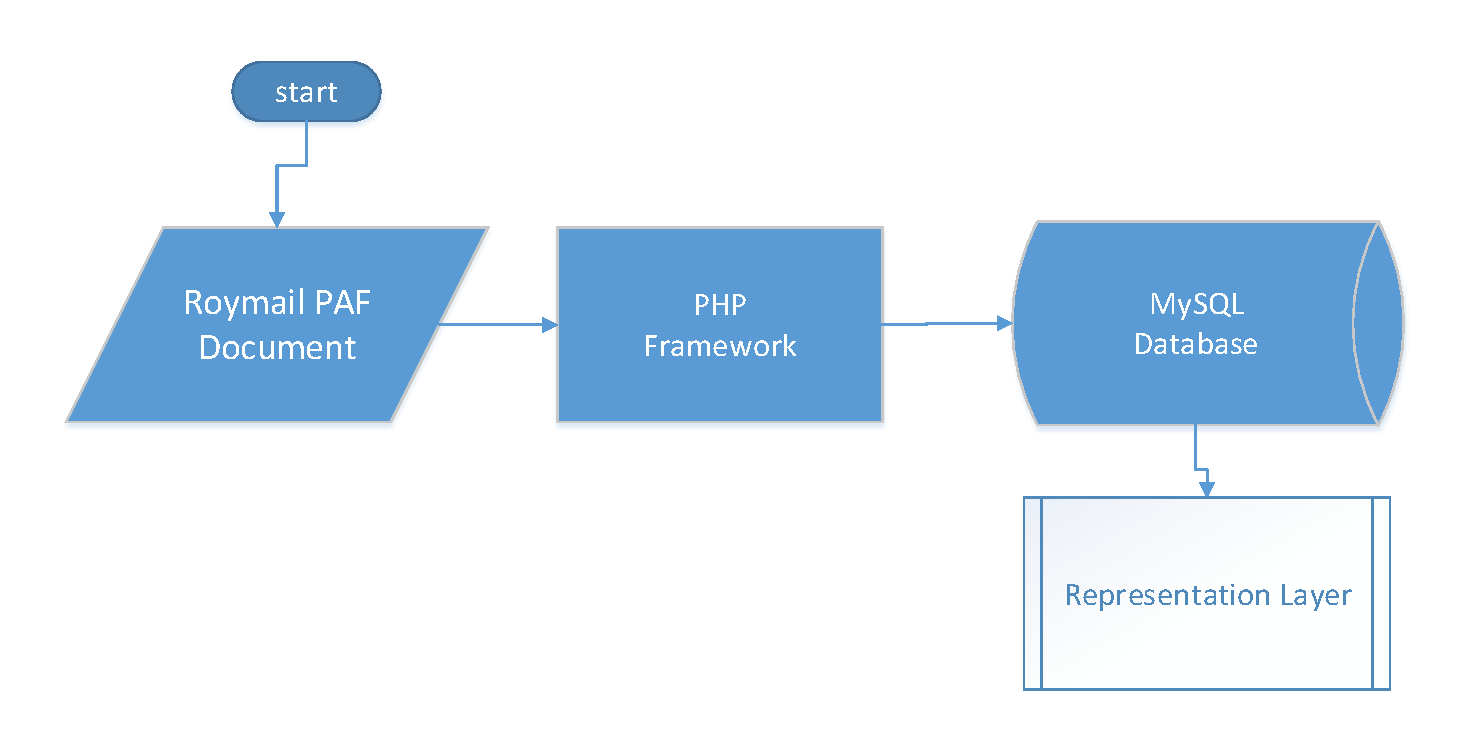
\includegraphics[scale=0.6]{chapter4/data_analysis_exp1}
\caption{Experiment One - UK Geographic Data Set Analysis}
\end{figure}

The Royal Mail PAF data set is quite large which required a special script to convert the file into a MySQL database  to enable future re-use and retrieval. The customised code  removed unwanted and repeated information from the PAF file and normalised the database accordingly for representation purposes in the next step. The refined database consisted of 1.7 million rows which were imported into the MySQL database. The extracted sample code for the raw data conversion into a normalised MySQL format is presented in Listing 1 and Listing 2.

%Python code highlighting
\begin{listing}
\begin{minted}
[
frame=lines,
framesep=2mm,
baselinestretch=1.2,
bgcolor=LightGray,
fontsize=\footnotesize,
linenos
]
{python}

require __DIR__.'/db-config.php';
set_time_limit(3600);
$options = array(
        PDO::MYSQL_ATTR_INIT_COMMAND => 'SET NAMES utf8',
        PDO::ATTR_ERRMODE => PDO::ERRMODE_EXCEPTION,
);
$dbh = new PDO('mysql:dbname='.DB_NAME.';host='.DB_HOST, 
DB_USER, DB_PASS, $options);

$include_columns = array(
        'ORD' => 0,
        'ORC' => 1,
        'SBN' => 2,
        'BNA' => 3,
        'NUM' => 5,
        'DST' => 6,
        'STM' => 7,
        'PTN' => 10,
        'PCD' => 11,
        'CTT' => 14,
        'LGE' => 25,
);

\end{minted}
\caption{PAF Raw Data Set Conversion Sample Code}
\end{listing}

%Python code highlighting
\begin{listing}
\begin{minted}
[
frame=lines,
framesep=2mm,
baselinestretch=1.2,
bgcolor=LightGray,
fontsize=\footnotesize,
linenos
]
{python}

$handle = fopen(__DIR__.'/Luton.csv', 'r');
$row = 0;
$max_rows = 0;
while (($buffer = fgets($handle, 4096)) !== false) {
    $row++;
    $csv_row = str_getcsv($buffer, ',');
    
    $insert_data = array();
    foreach ($include_columns as $col_name => $col_index) {
        $insert_data[strtolower($col_name)] = (string) $csv_row[$col_index];
    }
    
    $sth = $dbh->prepare('INSERT INTO geodata_uk 
    ('.implode(',', array_keys($insert_data)).')
    VALUES('.implode(',', array_fill(0, count($insert_data),
    '?')).')');
    $sth->execute(array_values($insert_data));
    
    if ($max_rows > 0 && $row >= $max_rows) {
        break;
    }
}
fclose($handle);


\end{minted}
\caption{PAF Raw Data Set to MySQL Selected Code 2}
\end{listing}

There were over 150 columns which were reduced to only 9 as depicted in Figure 4.2. This is  important information which  the data representation layer retrieved from the database. The database had rows such as latitude and longitude which were important for location detection while street, county and postcode names were required in the visualised form on an interactive map.


\begin{figure}[H]
\centering
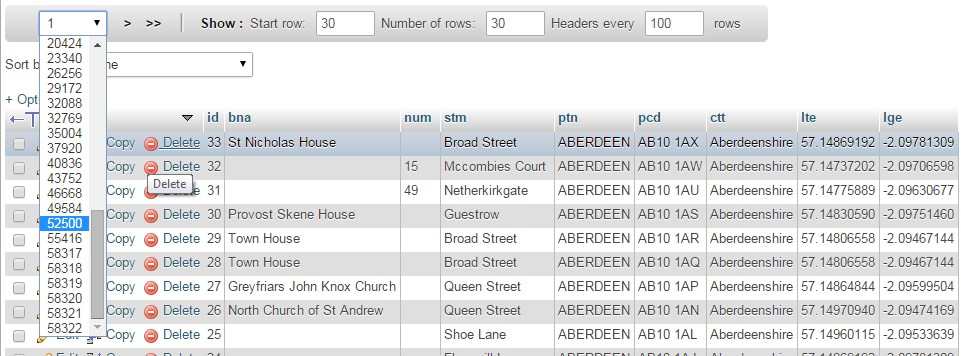
\includegraphics[scale=0.57]{chapter4/experiment_one_database}
\caption{Experiment One - UK Geographic Data Set MySQL}
\end{figure}

The refined information from the MySQL database is then retrieved by additional functions on the interactive map. Information such as latitude and longitude are used for location placement, while postcodes and other information are overlayed on the interactive map.

\subsubsection{Experiment Two - Business Transactional Data}

The business transactional data set and its acquisition is discussed, which is further explained in Chapter 5 in the business transactional experiment. The data set has been taken from a UK based business and covers approximately 7 years of transactional data consisting of around 30 million records of staff information such as logs. Sales operational data has also been imported and utilised in the data analysis and visualisation process. The process of acquiring and analysing data slightly differs from ordinary data sources as the data sets are already optimised and normalised since it is in an enterprise environment. This means the business has existing tools and frameworks which are responsible for data generation and business management and make them available to internal and external applications. Figure 4.3 shows the process of data analysis, where admin or the manager has the ability to pick and choose relevant information for the visualisation process.

\begin{figure}[H]
\centering
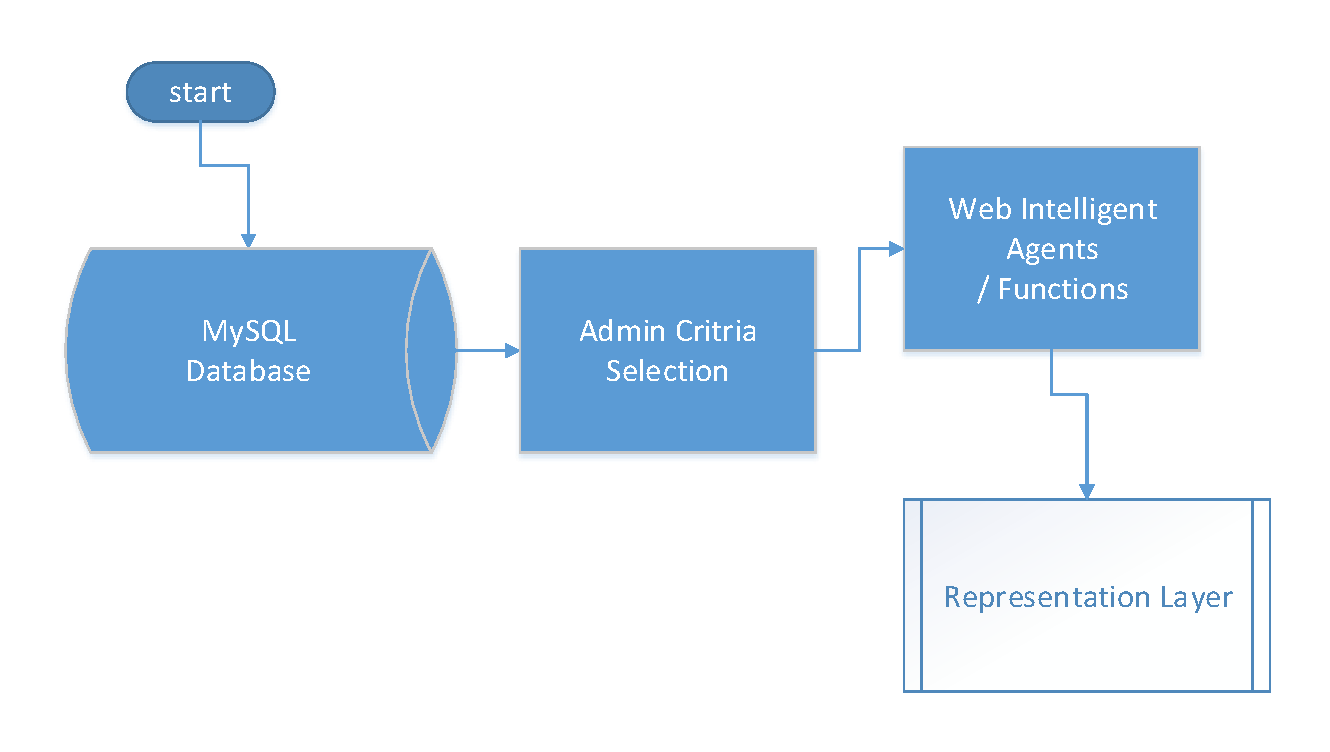
\includegraphics[scale=0.6]{chapter4/data_analysis_exp2a}
\caption{Experiment Two - Business Transactional Data Set in Enterprise Environment}
\end{figure}

Figure 4.4 demonstrates an example database table taken from the MySQL database showing staff members and sales target figures. The admin staff or the manager has options at the interact++ layer to select or deselect a particular staff member through the proposed system - thus the system is directly accessing information through a bespoke interface for the admin and the users. 

\begin{figure}[H]
\centering
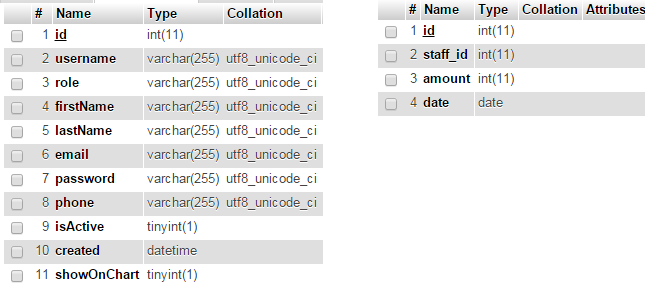
\includegraphics[scale=0.6]{chapter4/exp2_data_analys_db}
\caption{Experiment Two - Business Transactional Data Set Example Tables}
\end{figure}

The user selection and how information is pre-selected or on-demand selected for visualisation is further explained at the interact++ layer. Visualixer is a dedicated tool specially created for individuals and for data sets which are not related to any business application. In other words, data is directly imported into the data analysis model for processing, filtering and mining, which is then pushed into a database for re-use at the representation layer of our visualisation model through bespoke web intelligent agents.


\begin{figure}[H]
\centering
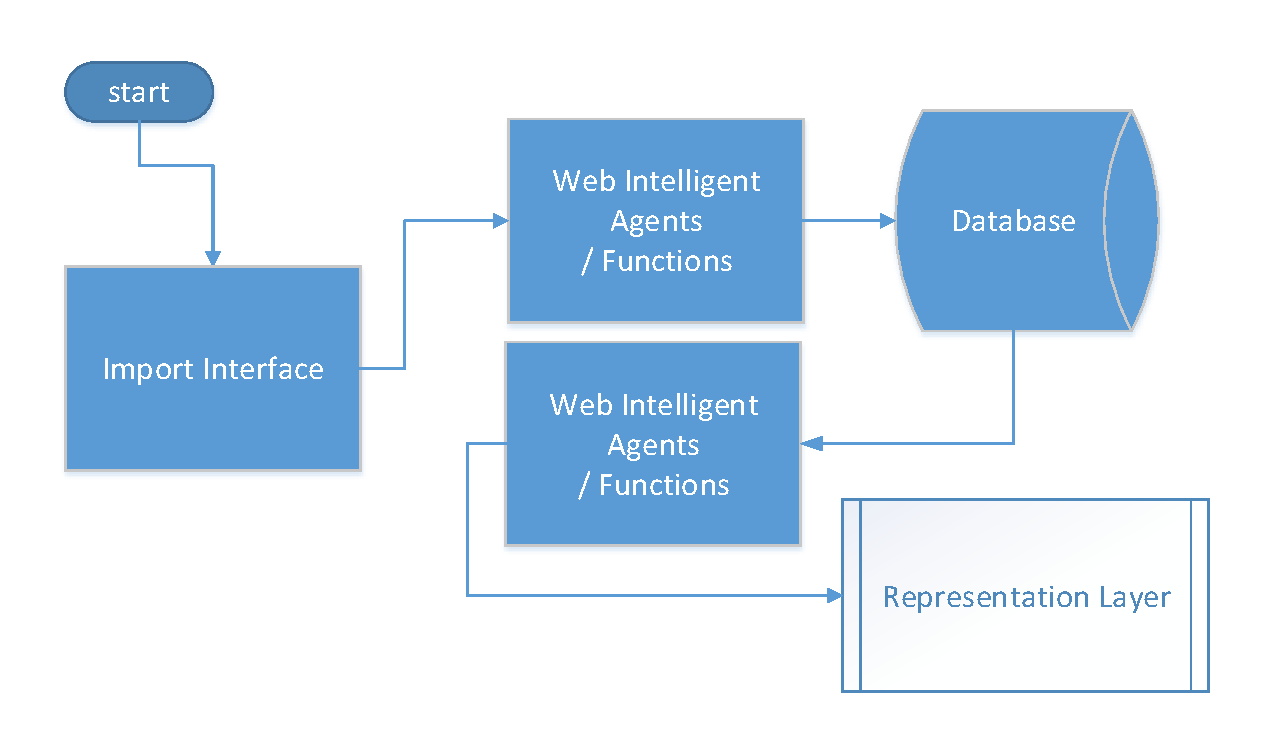
\includegraphics[scale=0.7]{chapter4/data_analysis_exp2b}
\caption{Experiment Two - Data Analysis Process in Visualixer}
\end{figure}

As shown in Figure 4.5, the data is first imported by the user through an interface layer and it goes into the data analysis model.  Where it is refined, unwanted information is removed and normalised and clean data is passed onto the MySQL database where it can be retrieved by the system functions at a later stage for visualisation. A sample import code has been shown in Listing 3, however the tool is created in a PHP framework which comes with thousands of lines of code and it is not possible to demonstrate the full system code. Instead, system features are demonstrated.

%Python code highlighting
\begin{listing}[ht]
\begin{minted}
[
frame=lines,
framesep=2mm,
baselinestretch=1.2,
bgcolor=LightGray,
fontsize=\footnotesize,
linenos
]
{python}
  .....
        public function upload()
        { 
            $this->load->model('import_model');
            $this->load->helper('file');
            $user_data = $this->session->userdata('id');
           
            //$path = './upload/'.$user_data;
            $path = './upload/temp';
            if(!is_dir($path)) //create the folder if it's not already exists
            {
              mkdir($path,0777,TRUE);
            } 
            $this->load->helper('form');
            $config['upload_path'] = $path;
            $config['allowed_types'] = '*';
            $config['max_size']	= '';
            ......



\end{minted}
\caption{Experiment Two - Visualixer Import Function Highlights }
\end{listing}

\subsection{Data Representation}

In this section, a brief discussion on the representation of the data which has been analysed by acquisition and data analysis layer in the previous step is shown. Firstly, in  Experiment One, a data set will be discussed which has been adapted from the Royal Mail PAF address which has been refined in the data analysis step; data required for this experiment has already been normalised and is available in the MySQL format for the web intelligent agents (PHP functions) to be retrieved for the representation layer, as illustrated in Figure 4.6.

\begin{figure}[H]
\centering
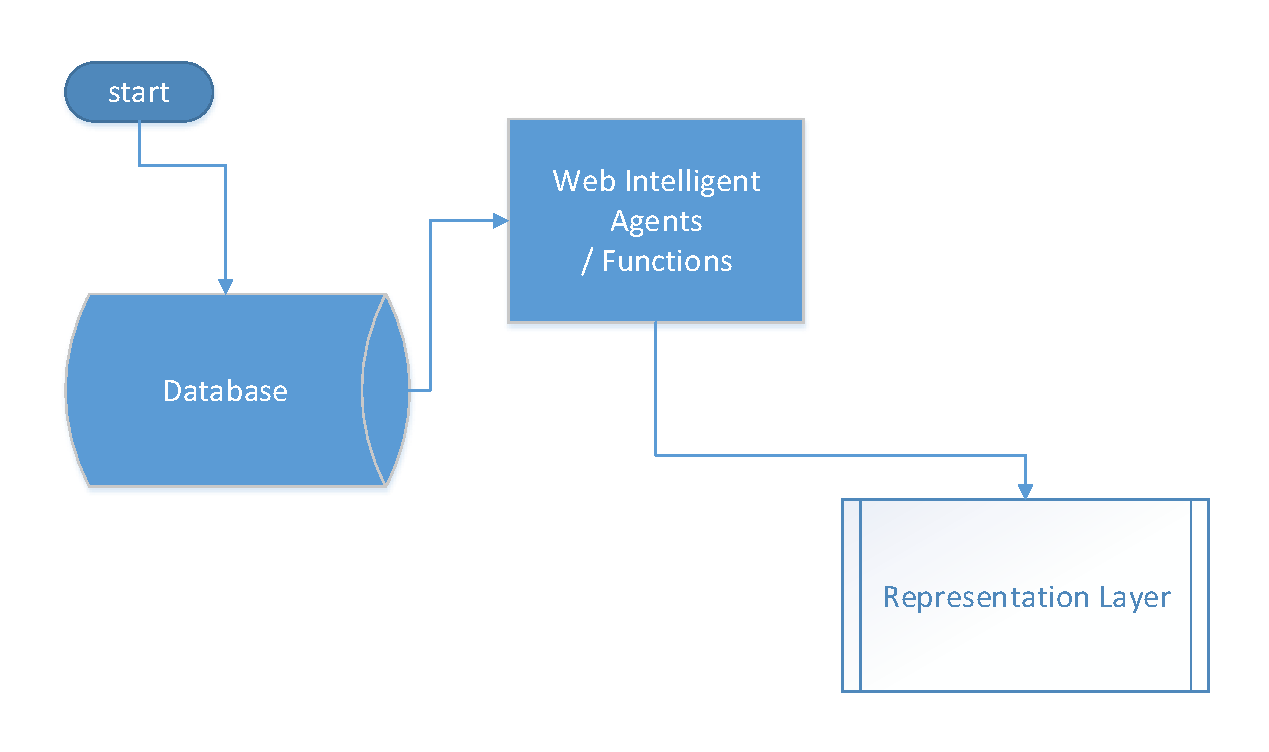
\includegraphics[scale=0.6]{chapter4/respresentation_exp1}
\caption{Experiment One - Data Representation Process}
\end{figure}

The data retrieved from the database has been represented with an interactive map. The data mashup aspects of the visualisation model are introduced and processed at this layer. Mashup tools are convenient to program and develop quick and short applications which support other processing and analysis functions within the proposed system. A short interactive map initialisation code shows the process in Listing 4.

\begin{listing}[ht]
\begin{minted}
[
frame=lines,
framesep=2mm,
baselinestretch=1.2,
bgcolor=LightGray,
fontsize=\footnotesize,
linenos
]
{python}
  .....
  function initializeMap() {
  map = new google.maps.Map($('#map-canvas')[0], mapOptions);
  map.controls[google.maps.ControlPosition.TOP_LEFT].push($('#topbar')[0]);

  /* attach searches */
  $('#address').autocomplete({
    source: mapAreas,
    select: function(event, ui) {
      var areaName = ui.item.value.toUpperCase();
      var matchLen = 0;
      var matchArea;
      for(var areaKey in mapAreaBounds) {
        if (name.length == 1 && areaKey == areaName) {
          matchArea = areaKey;
          matchLen = 1;

          break;
        } else {
          var pos = areaKey.indexOf(areaName);
          var len = areaKey.length;
          if (pos == 0) {
            if (matchLen == 0 || len > matchLen) {
              matchArea = areaKey;
              matchLen = len;
            }
          }
        }
      }

            ......



\end{minted}
\caption{Experiment One - Interactive Map Initialisation Example Code }
\end{listing}

The data representation process is explained at the enterprise level or in applications where data is already normalised and in a known state. The data is retrieved from the database through web intelligent agents (PHP functions) and then made available to users at the interact++ layer; the user has the ability to pick and choose what information users may want to visualise and the information is then pushed into the database again for future re-use purposes. Web intelligent agents then remember user choice or preferences and push specified data into the representation layer, which then generates visualised information for the user at the interact++ layer; the flow chart of the process is manifested in Figure 4.7.

\begin{figure}[H]
\centering
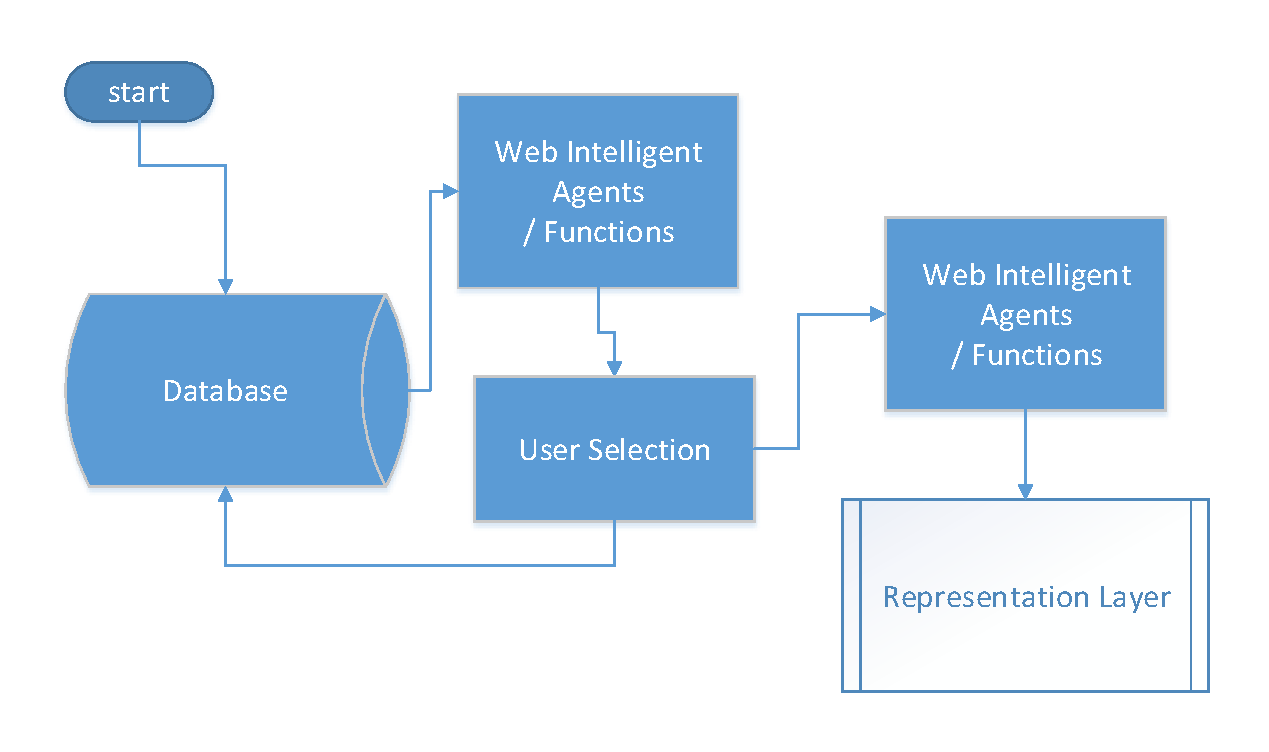
\includegraphics[scale=0.6]{chapter4/data_representation_exp2a}
\caption{Experiment One - Visualisation Model from Various Perspective}
\end{figure}

The code sample in Listing 5 shows the basic functions for data representation at this layer. The demonstrated code is only an example and an extracted partial code of how this process works and how data is retrieved from the database for  representation purposes.


\begin{listing}[ht]
\begin{minted}
[
frame=lines,
framesep=2mm,
baselinestretch=1.2,
bgcolor=LightGray,
fontsize=\footnotesize,
linenos
]
{python}
  .....
use Symfony\Bundle\FrameworkBundle\Controller\Controller;
use Symfony\Component\HttpFoundation\Request;
use Symfony\Component\HttpFoundation\ResponseHeaderBag;
use Sensio\Bundle\FrameworkExtraBundle\Configuration\Route;
use Premier\CoachhireBundle\Form\Type\Quote\ListFilterType;
use Premier\CoachhireBundle\Entity\Quote;
use Premier\CoachhireBundle\Entity\Invoice;
use Doctrine\ORM\Query;
use DateTime;
use PDO;

    public function latestSalesStatsAction(Request $request)
    {
        $em = $this->getDoctrine()->getEntityManager();

        $months = range(1, 12);
        $years = range(date('Y')-2, date('Y'));
        $defaultData = array('month' => date('n'), 'year' => date('Y'));

        $form = $this->createFormBuilder($defaultData)
            ->add('month', 'choice', 
            array('choices' => 
            array_combine($months, $months), 'required' => false))
	        ->add('year', 'choice', array(
	        'choices' => array_combine($years, $years), 
	        'required' => false))
	        ->getForm()
    	;

        $stats = array(
            'enquiry'   => array(0, 0),
            'processing'   => array(0, 0),
            'booked'    => array(0, 0),
            'declined'  => array(0, 0),
            'following' => array(0, 0),
            'processing_active' => array(0, 0),
            'total_active'   => array(0, 0),
        );
        ......



\end{minted}
\caption{Experiment Two - Data Representation Preparation Example Code }
\end{listing}
\clearpage

In a non-enterprise environment where data is not in SQL format, the Visualixer converts data into MySQL in the previous section (Acquisition and Data Analysis). The Visualixer at the interact++ layer gives the user the choice to select information for visualisation. The user retrieves information from the database through web intelligent agents (PHP functions) and once the information is retrieved, the user then submits the information into the representation model where the information is visualised, as shown in Figure 4.8.

\begin{figure}[H]
\centering
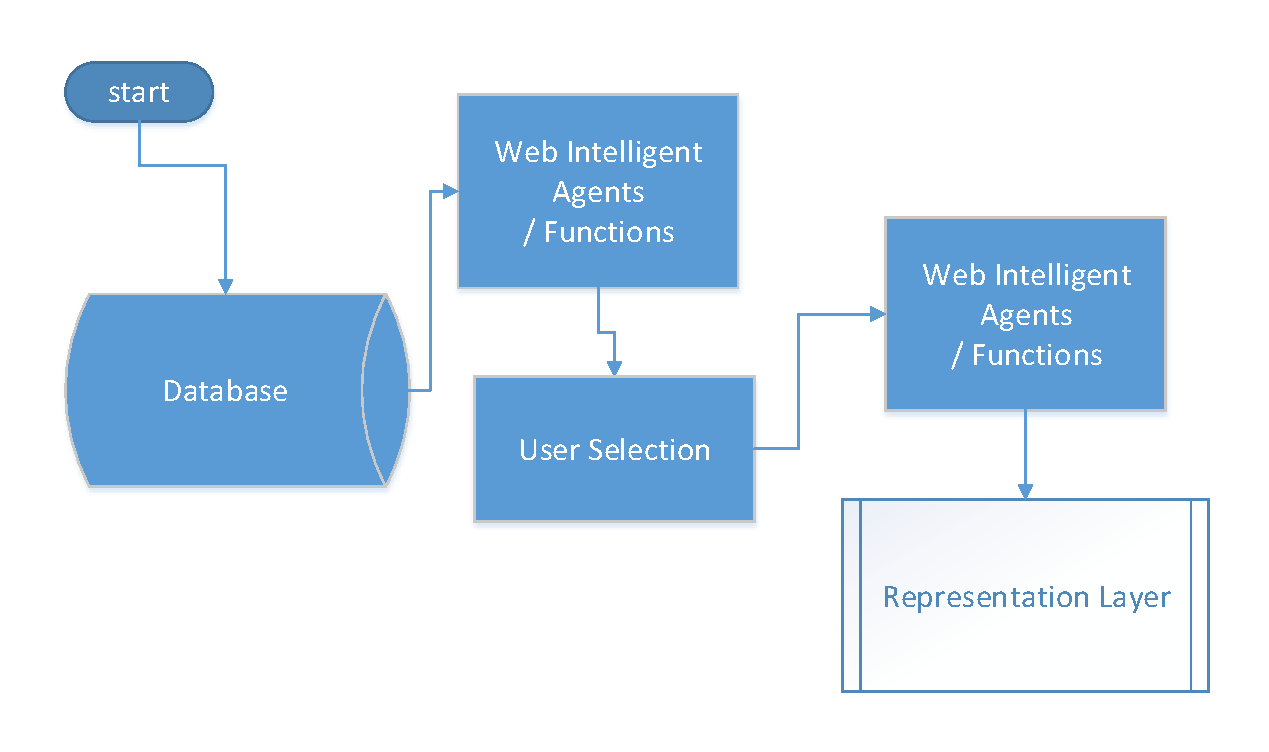
\includegraphics[scale=0.6]{chapter4/data_representation_exp2b}
\caption{Experiment Two - Data Representation in Visualixer}
\end{figure}

The data representation of different data sets is explained with various flow charts and with brief code examples. In the next section the interact++ layer will be discussed, showing how users interact with the system. 

\subsection{User Interaction}

User interaction is an important aspect of any application. User interaction relates to all elements depending how users react to an application and how applications react to the user responses \cite{hix1993developing}. The interactive layer is mostly designed and developed using front end technologies such as HTML and CSS with the help of JQuery and other supporting tools. A variety of mashup applications are also utilised in the development process. Bootstrap is also used in the creation of user interfaces. The system adaptability and user experience has been enhanced with JQuery and Javascript functions and applications by giving auto-complete options to users. In Experiment One - with UK geographic data - AJAX (mostly JAVA functions) is used for better interface, user and application interaction. However, more conventional technologies such as HTML5 and CSS3 are used in Visualixer (the tool which is developed for non-enterprise data sets). In Experiment Two - with business transactional data - a more enhanced user interface is provided as most of the system is controlled by the users to issue instruction to the application for both data analysis and data representation. 

\subsection{Exporting Reports}

Data export features of the system are discussed. Generating and analysing data and information is a very useful process, however information not stored for future use does not add much value to the application. The export feature of reports and data is a vital part of the visualisation model. Therefore this has been precisely considered and developed to equip system users to export and save data for external use. Experiment One -  with the UK geographic data, the user has the option to export visualised maps into various formats such as JPEG, GIF, PNG, PDFs. The exported files are of high resolution and quality print. Experiment Two - with an enterprise environment, this also gives the ability to end users to export charts and graphs into JPEG, GIF, PNG and PDFs. The system also gives the user an option to extract utilised data in CSVs and they are accessible through APIs for external applications. These export features are powered by customised and bespoke functions and partial mashup applications are also used in the system development. Using Visualixer in Experiment Two also gives the same ability to the users to export generated charts and graphs in various formats. 

\section{Design and Development Overview of Experiment One}

A brief overview of Experiment One is presented in Figures 4.9 and 4.10, showing the visualisation model, development process and technologies, and from the end user perspective. 

\begin{figure}
\centering
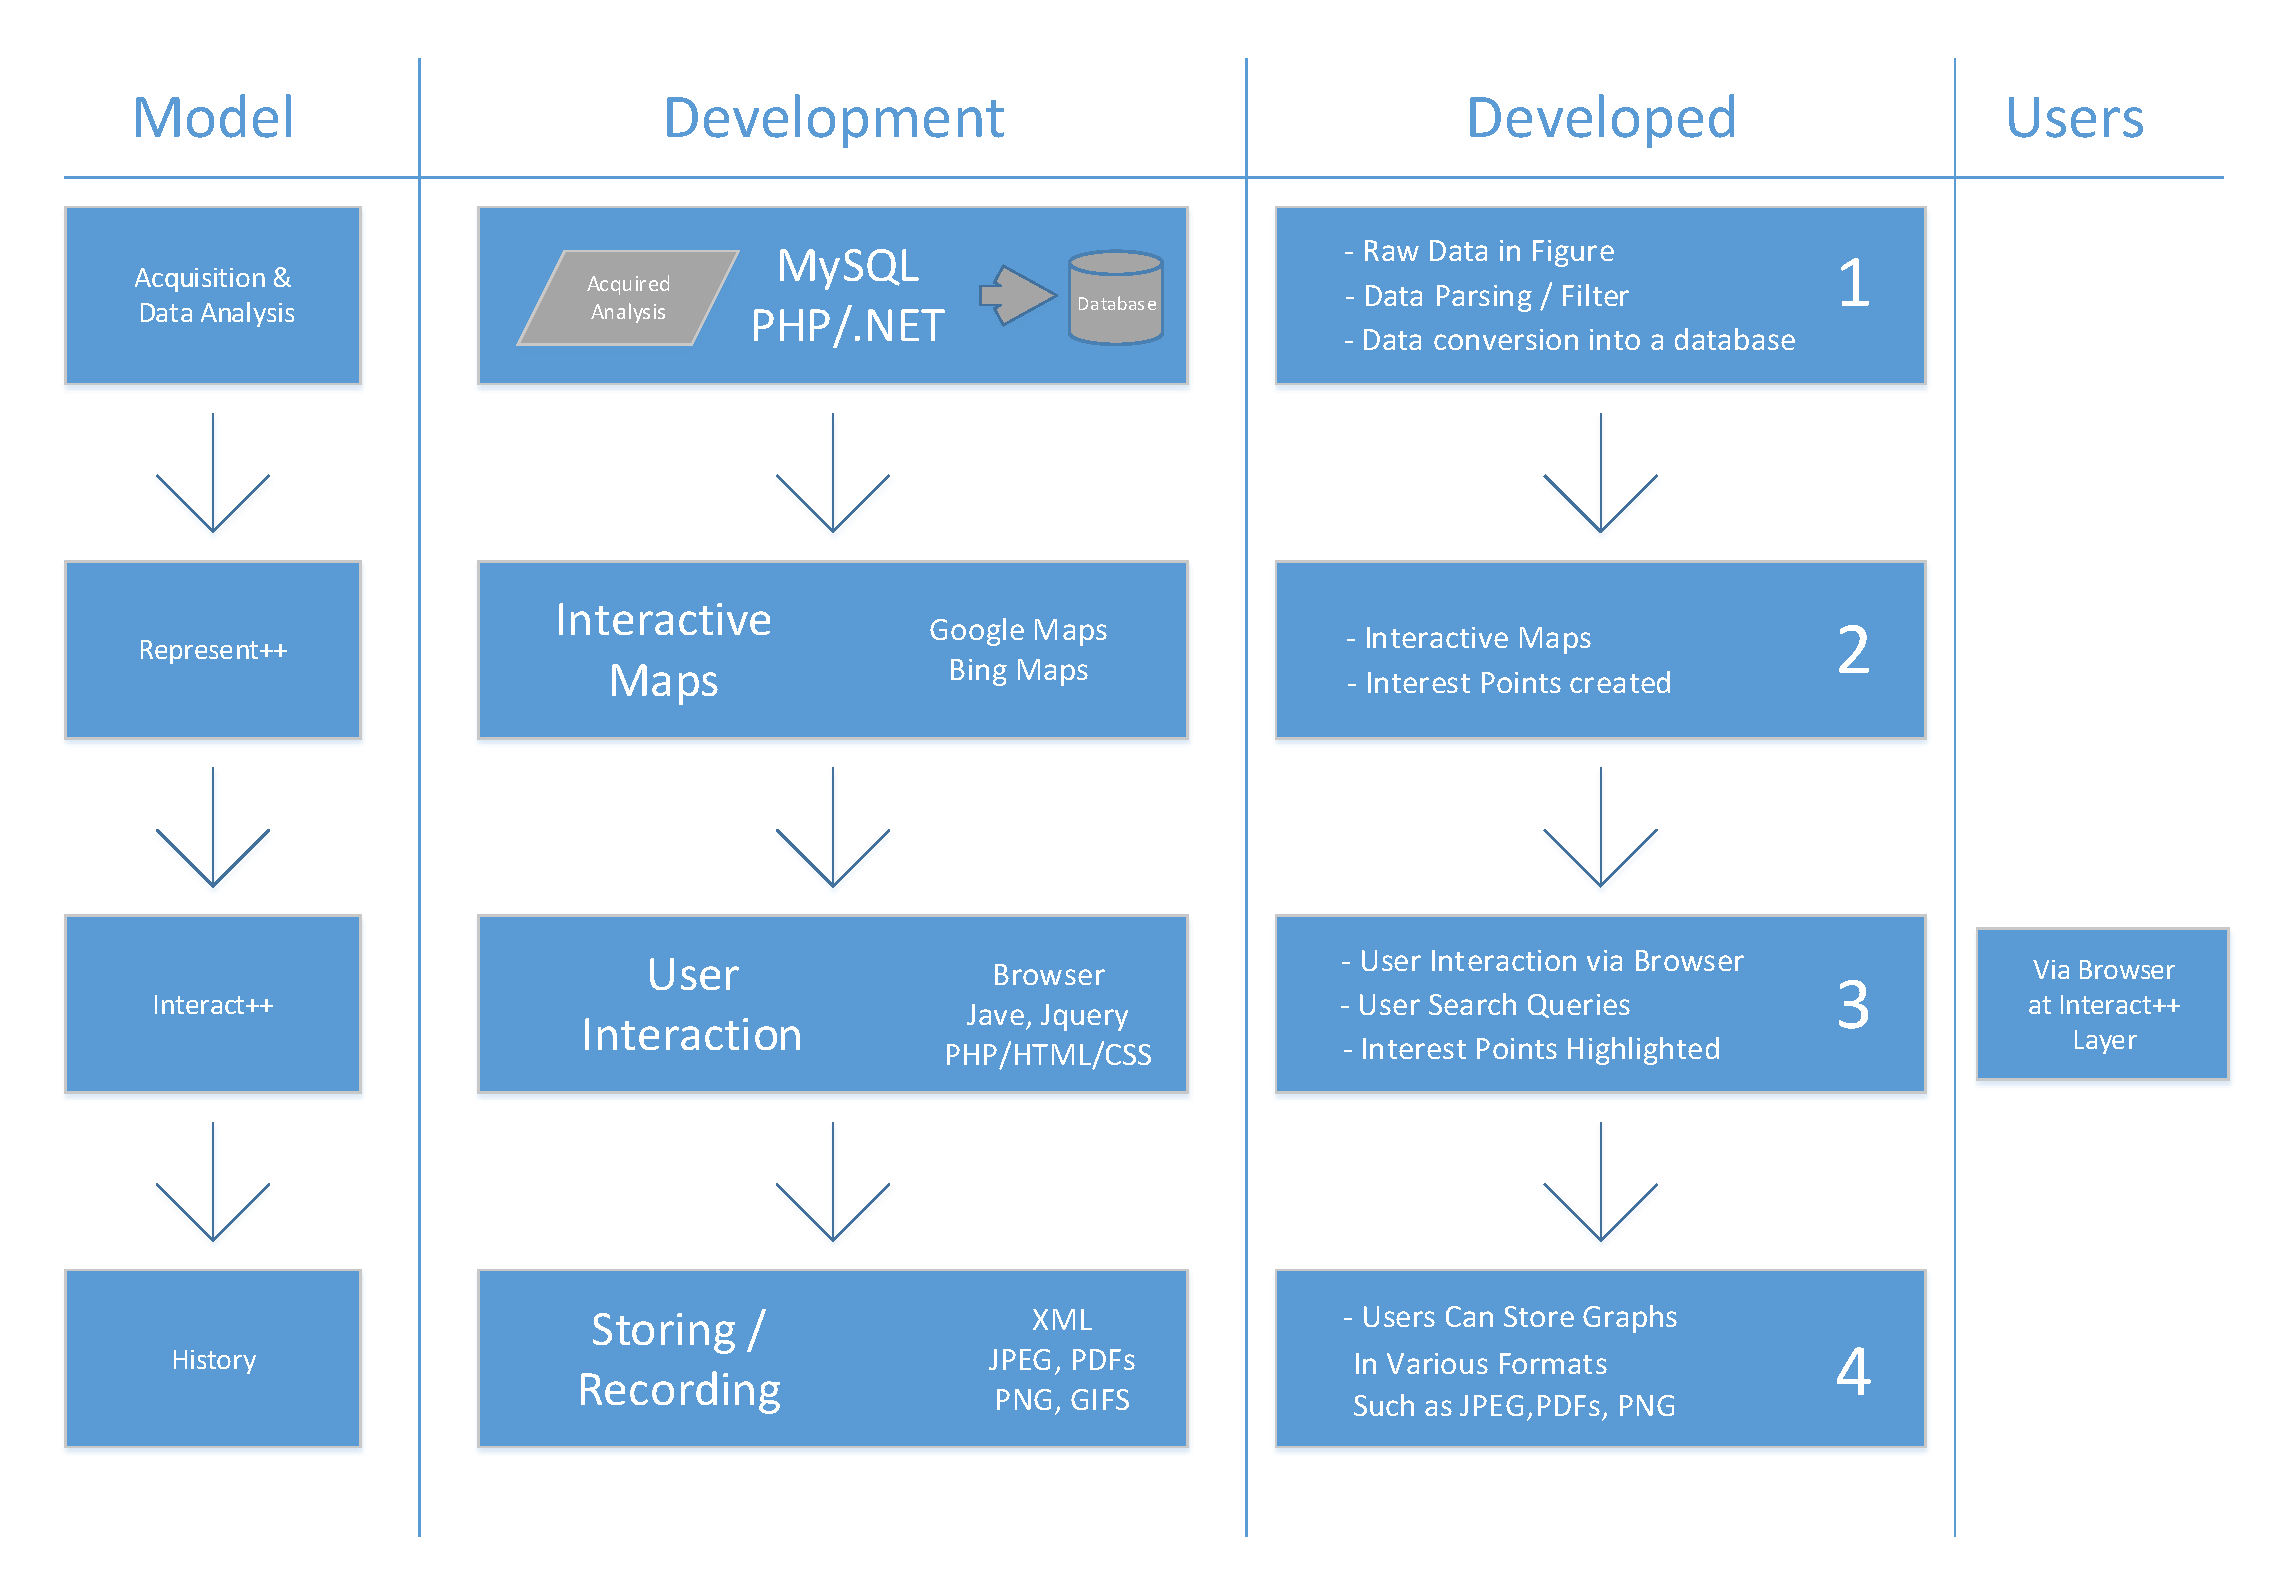
\includegraphics[scale=0.37]{chapter4/system_full_overview}
\caption{Experiment One - System Overview}
\end{figure}

\begin{figure}
\centering
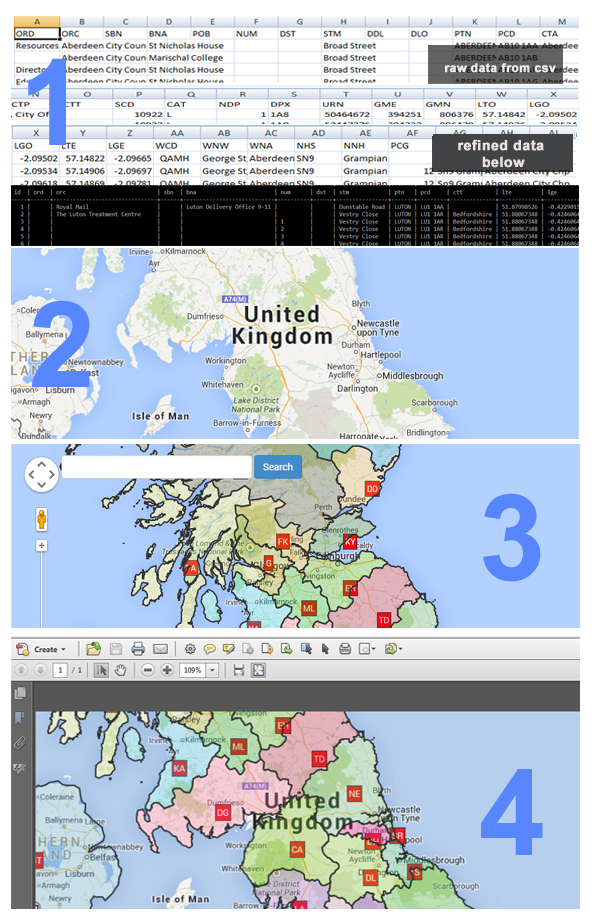
\includegraphics[scale=0.7]{chapter4/actual_overview}
\caption{Experiment One - Actual System Overview}
\end{figure}

In Figure 4.10, actual screen shots are taken from the application. The numbers 1-4 on the screen shots refer to layers in the information visualisation model. The process is started from the acquisition and data analysis point. Data is visualised at the represent++ layer. User interaction takes place at the interact++ layer, while export options are available at the history layer. 

\section{Design and Development Overview of Experiment Two}

A brief overview of Experiment Two is discussed in this section. Experiment Two in Chapter 5 is further divided into two parts. The first part of the experiment deals with data sets which are already in a well developed application and data sets are either directly accessed from the MySQL database or through APIs and web services. The model design shows the main four stages, starting from acquisition and data analysis, data representation, user interaction and exporting of generated reports. The development process is also defined and instructions are given to define what kind of technologies could be used in order to replicate or utilise the same visualisation process and model. Developed application and its user levels with different privileges are also explained in the overview chart in Figure 4.11.

\begin{figure}
\centering
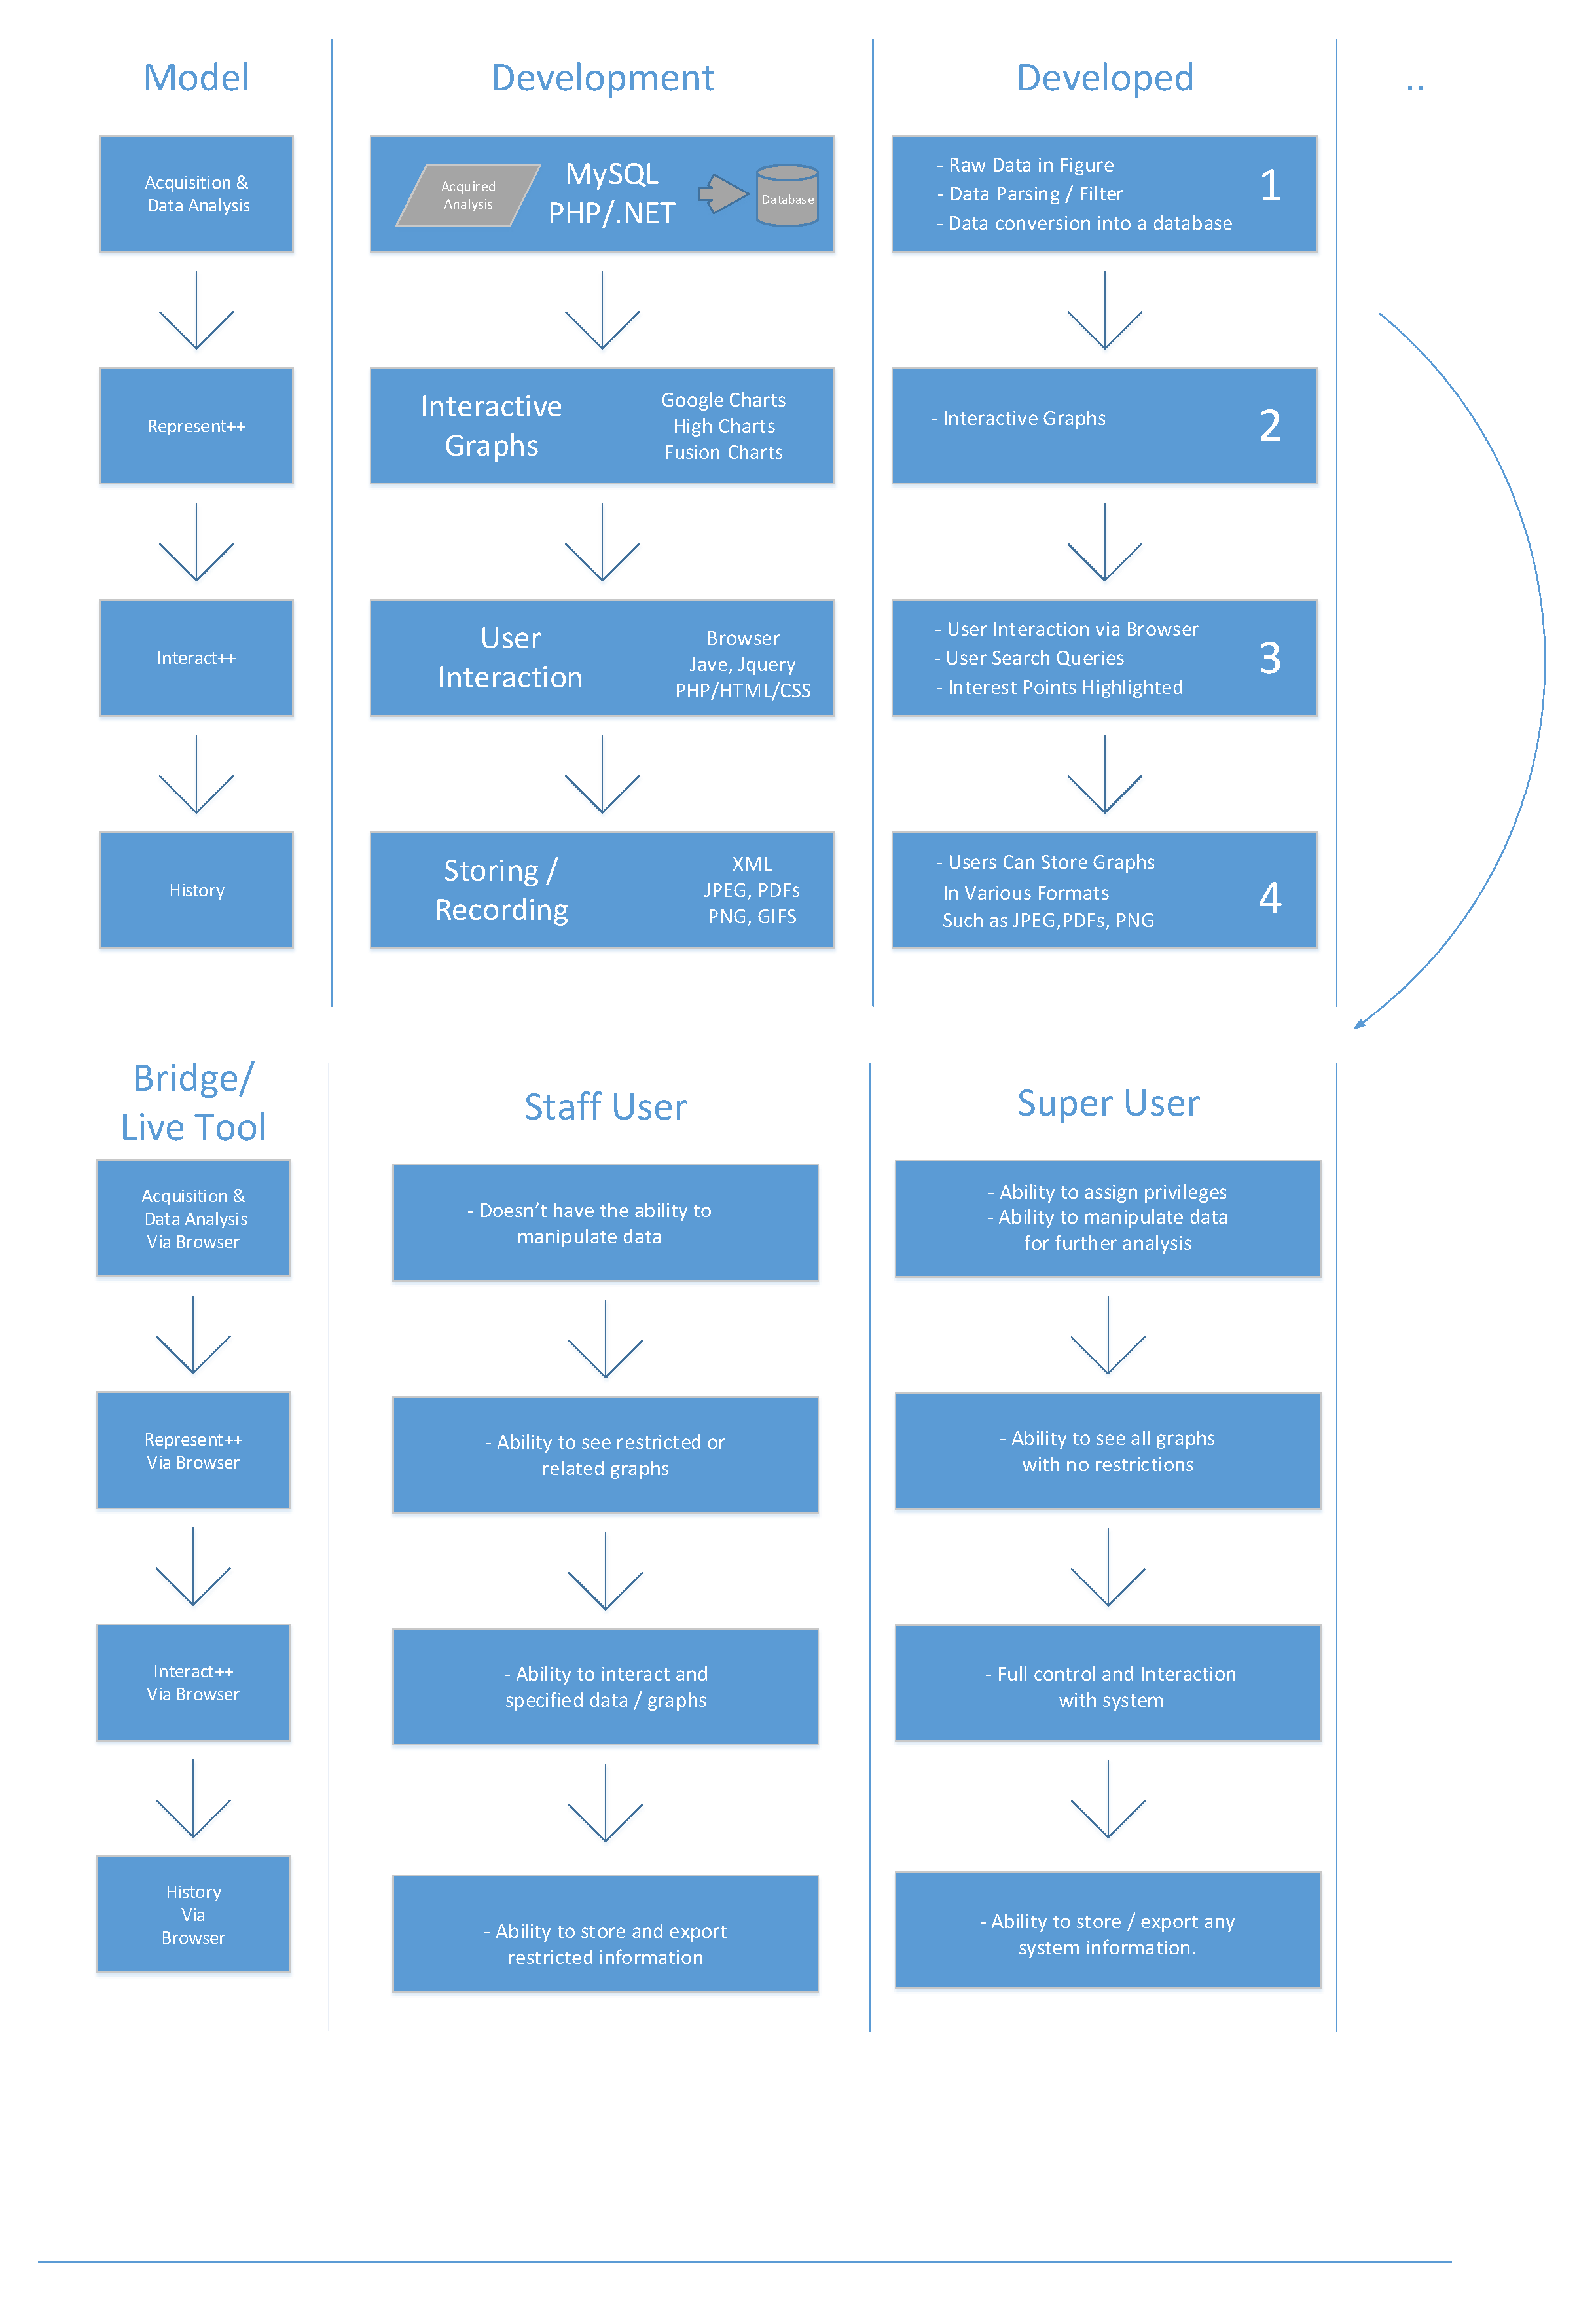
\includegraphics[scale=0.37]{chapter4/overview_ex2a}
\caption{Experiment Two  - System Overview}
\end{figure}

Figure 4.12 illustrates actual screen shots, starting from MySQL databases, showing how users see the information at the front end and then the data representation and interaction with the user in Step 3. Step 4 shows options to export information such as graphs and structural data into various formats. The same area of the figure also shows other relevant sections of data visualisation including multi-coordinate visualisation and multiple attribute data visualisation made available to users at the interface layer.

\begin{figure}
\centering
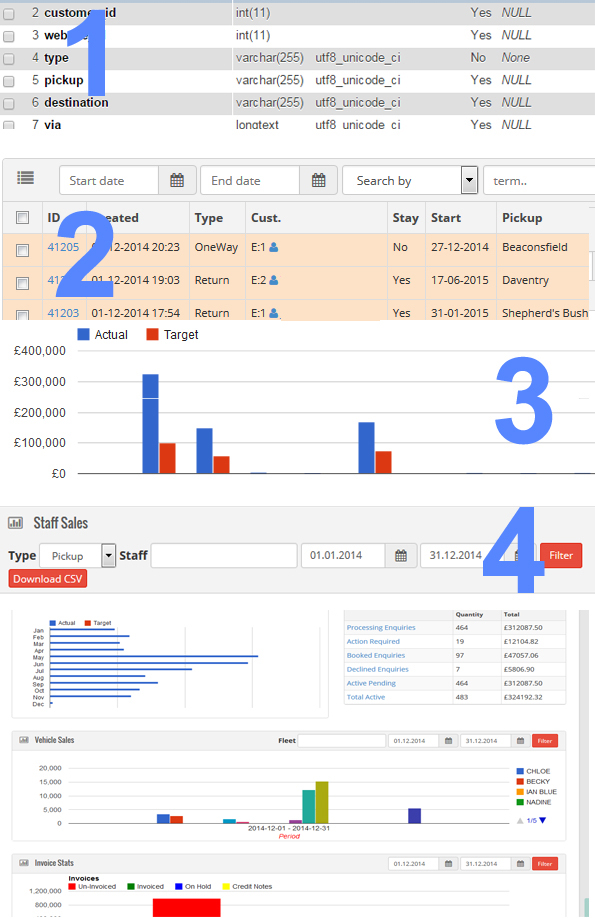
\includegraphics[scale=0.7]{chapter4/exp2a}
\caption{Experiment Two  - Enterprise 2.0 Application Screen shots}
\end{figure}


In the process for data sets which are in a non-enterprise format or not in normalised form, the data sets are imported into the acquisition and analysis layer for refinement and analysis for data representation at a later layer. Figure 4.11 demonstrates various steps from the initial theoretical model to the development process and in-development phases, showing different type of user access. The information visualisation model layers are highlighted in the first column while development scenarios explained in the second column. Developed aspects of the visualisation model are highlighted in the third column. Bridge refers to Enterprise 2.0 environment where web intelligent agents are configured to retrieve information from the data set in a real time environment. Live tool refers to Visualixer which is a dedicated tool based on the four layers of proposed visualisation model. Various aspects of users highlighted in the last two columns of the flowchart. Figure 4.13 manifests screen shots from the live system (Visualixer). The first step deals with raw data and converts it into normalised and database format; the web intelligent agents (PHP functions) read information from the database allowing users to select the required fields for visualisation and then pass them on to the data representation layer for visualisation. The user's interaction is achieved at the interact++ layer with the help of HTML5, CSS3, AJAX and JQuery technologies for clean and easy to use interfaces.

\begin{figure}[H]
\centering
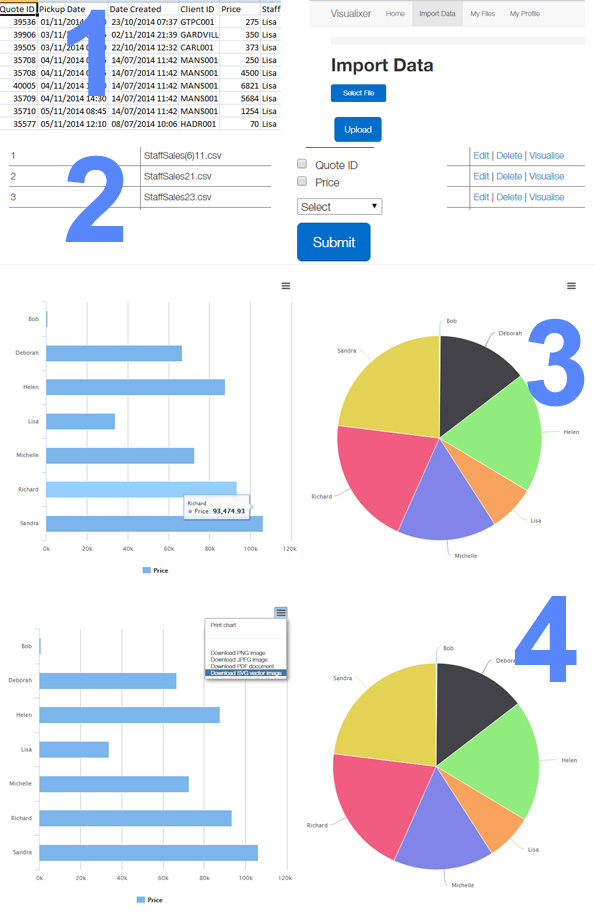
\includegraphics[scale=0.7]{chapter4/exp2b}
\caption{Experiment Two B  - Visualixer Tool Screen shots}
\end{figure}

\section{Summary}

The visualisation model has been revisited from Chapter 3 with abstract proposed system flow charts presented from the overall model and each layer of the model. The data processing and visualisation along with user interaction and data export are explained with a system flowchart and the technologies used in the mechanism.

In the second part of the chapter, each layer of the visualisation model has been explained with an example code from the actual applications developed for the experiments accompanied by flowcharts for each step. An overview of the two experiments in Chapters 5 and 6 are briefly discussed with screen shots from the application. The system process is examined at each individual layer of the information visualisation model. 

The objective of this chapter was to give a better understanding to the reader of how the model has been adapted and developed. The two experiments are demonstrated with screen shots for a brief overview of the system structure and design. The next chapter shows detailed information about the data set used in the experiment and how data is visualised by the system covering all four layers of the visualisation model proposed in this research.
 
% Chapter 4

\chapter{Experiment One - Information Visualisation of UK Geographic Data} % Main chapter title

\label{Chapter5} % For referencing the chapter elsewhere, use \ref{Chapter1} 

\lhead{Chapter 5. \emph{Experiment One - UK Geographic Data}} % This is for the header on each page - perhaps a shortened title

%----------------------------------------------------------------------------------------

\section{Introduction}

In this chapter, the research model will be exposed to real and large data set which is acquired from the Royal Mail Group UK Limited. The data set is not available freely in the market, however it could be purchased for applications development and research purposes. The visualisation model's all four steps are discussed and how the data set visualisation starting from acquisition and data analysis to data representation and user interaction with option to save and export reports. The postcode experiment is built on the proposed system of a single data set - albeit a large one as contains 27 million data rows, making it an ample size to analyse. However, attached to this data set were several smaller data sets, all of which were to be analysed at the same time as the postcode data. These secondary data sets include information on churches, mosques, supermarkets and schools; all of which will be processed and visualised to create a singular location portal for different users. The process of visualising Royal Postcode Address File (PAF) data set involves various stages of data analysis, representation and interactive layers to bring the visualisation model to life. The process is a step-by-step activity explaining how the data is visualised. The outcome of such a complex and large data and how it could be beneficial to institutions and individuals. 

\section{Acquisition and Data Analysis}

The data sets acquired for this experiment were kindly offered by one of the commercial partners of the Royal Mail. This includes England, Scotland, Northern Ireland, Wales, Jersey, Guernsey and the Isle of Man. The postcode is part of a unique coding system designed for the sorting of mail. Invented and administered by the Royal Mail in 1974, postcodes are abbreviated forms of the whole address, and this system allows the UK to be split into designated delivery points. It was devised as an alphanumeric system, and by 1974 it had adopted national coverage \cite{mail1997postcode}. To help employees and sorting equipment to read and interpret typed or handwritten text on the post, the postcode was designed to make this easier. This is the reason the Royal Mail prefers the postcode to be written on a separate (preferably the last) line of the address. There are various formatting rules surrounding postcodes and layout - and this particularly applies to which letters can or can't be used within it. The reason for this is to cut the confusion caused by letters being mistaken for others or muddled up. For example, an O could be mistaken for a Q, or two of the letter V in succession could be mistaken for a W. Postcodes are also used for a variety of other purposes; some of which include calculation of insurance premiums, the designation of destinations in route planning software and even as the lowest level of aggregation in census enumeration. All of these purposes however, can be achieved through the breakdown and analysis of the data in a particular fashion. The royal mail postcode data has been briefly explained above, however there is further explanation available here \cite{royalmail}. The primary data set for this experiment will be, as mentioned previously, made up of the Royal Mail PAF (Postcode Address File) raw data, which will then be processed using our mashup system and projected onto interactive maps. However, there are a number of complimentary data sets from sources such as Google Maps, Bing, Yahoo and Yell in order to draw a complete picture for our map visualisation. This data includes locations like schools, churches, mosques, hotels, supermarkets, nurseries, surgeries, garages and bus stops, among others. The sub data sets and the Royal Mail data will be processed simultaneously, and the result of this will be more vertical and fully functional data for the final interactive maps. These maps will include multiple layers and allow users to dissect the data to any level.

The first stage of data analysis of this magnitude involves actually acquiring the data. To do this, one will need to follow various procedures and functions to obtain data, whether it is in a structural or a raw format. Data sources could be from various mediums; from a simple disk to a network stream. Quite often the source of the data will be dependent on the nature of the data itself. The Royal Mail PAF data set is quite large and this sort of data will usually only be available through network links or a data disk in its raw format. The data in questions is not available to the general public nor it is free to use. A selection of sample data extracted from the Royal Mail PAF data set. The data fields included are large, which are illustrated in Figures 5.1, 5.2 and 5.3.

\begin{figure}[H]
\centering
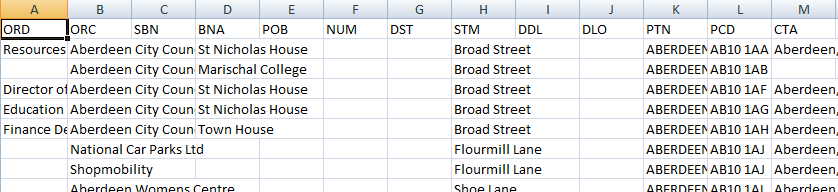
\includegraphics[scale=0.6]{chapter5/raw_date1}
\caption{Royal Mail PAF Data Set Attributes 1}
\end{figure}

\begin{figure}[H]
\centering
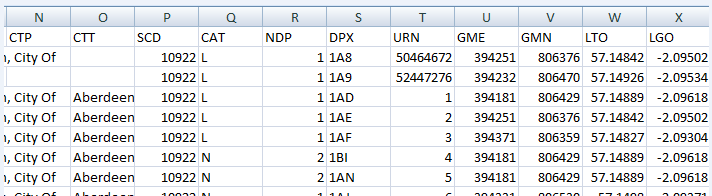
\includegraphics[scale=0.77]{chapter5/raw_date2}
\caption{Royal Mail PAF Data Set Attributes 2}
\end{figure}

\begin{figure}[H]
\centering
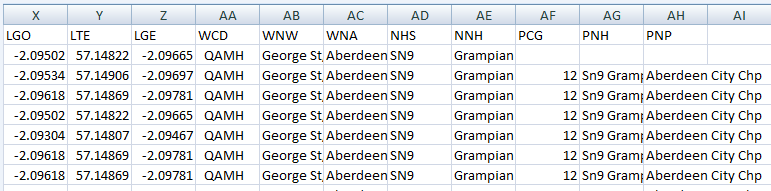
\includegraphics[scale=0.6]{chapter5/raw_date3}
\caption{Royal Mail PAF Data Set Attributes 3}
\end{figure}

The raw data in its full form contains around 36 columns as depicted in Figure 5.4, all representing a different type of data. This is from a postcode, town name to first lines of an address. It also includes more geographically relevant data, such as the UK latitude and longitude, as well as their EU counterparts. In addition to this, they contain more sensitive information about the area described, such as the local government and NHS locality; all of this is a part of the extensive data set. The Royal Mail data set is taken from an extensive database that charts every element of the UK in excruciating detail, using a grid mechanism to define everything about a local area. Using this database, one can identify the names of the local authority, grid points, original and current postal code areas even, the top tiered local government of any area within the UK, no matter how small. A data set of this size is difficult to sift through manually, and equally hard to understand in its raw state. Therefore, need a robust visualisation model to analyse such colossal data.

\begin{figure}[H]
\centering
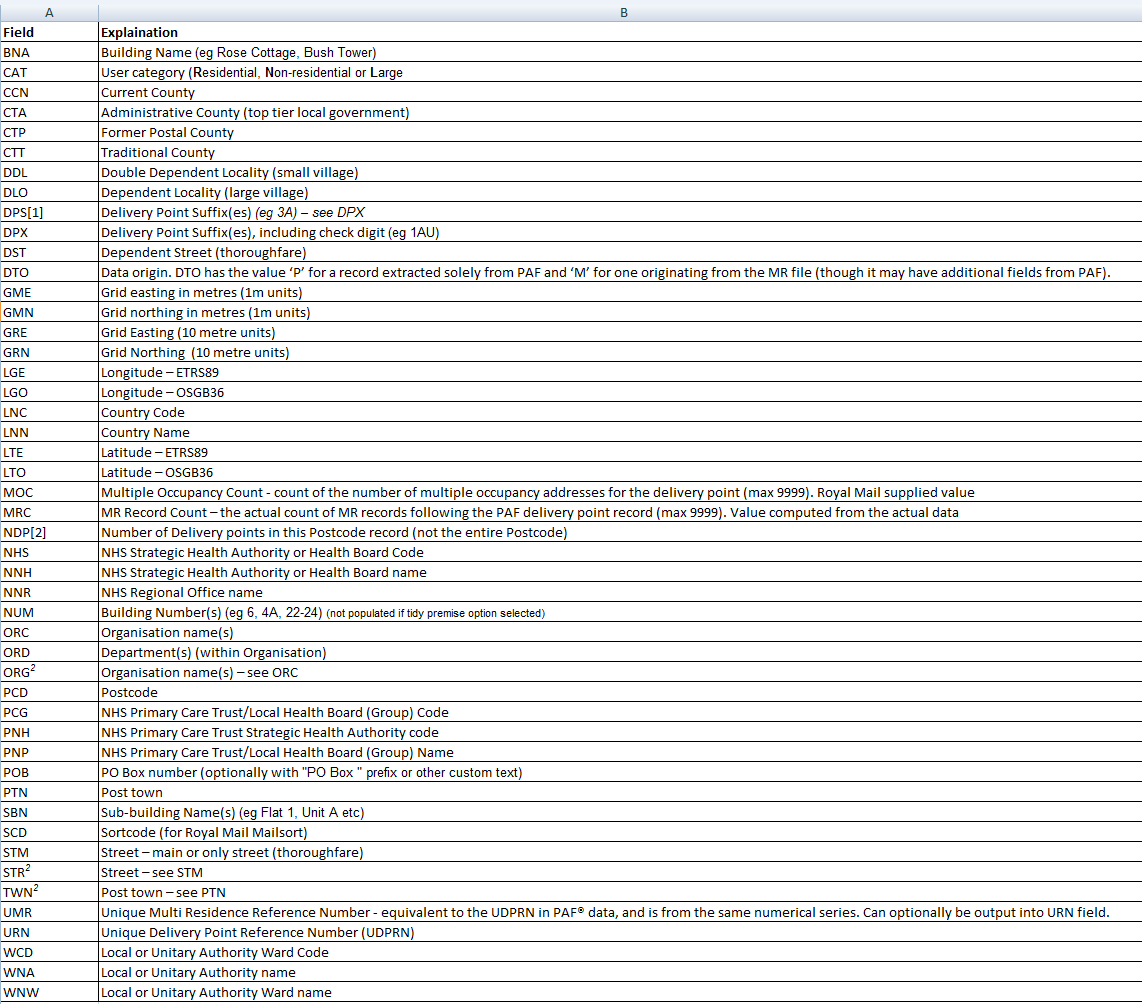
\includegraphics[scale=0.48]{chapter5/psotcode_data_fields}
\caption{Royal Mail PAF Data Set Fields}
\end{figure}
% figures here

The acquired data has been formatted, it is in a compact and readable position to continue. However the data is still not in the perfect state to be able to extract meaning from it, and use this to visualise and produce our map. Small programming codes could help to retrieve such information, it needs to be further refined. There are two more processes that need to be done before the data is ready to be taken to the next step. This will make the data much more compact and meaningful for analysis. As a part of this process, data filtering is essential, as the processing system will remove any duplicated or unwanted information from the data sets. The data is in a much more compact and usable state at this stage, applying filtration methods help to refine it further to make it fit for purpose as demonstrated in Figure 5.5. This also streamlines the data; removing any duplicate rows or columns or anything irrelevant to the analysis. For example, in Figure 5.5 the EU latitude and longitude is not needed for this experiment, so these columns will be removed from the data set during filtration. 

\begin{figure}[H]
\centering
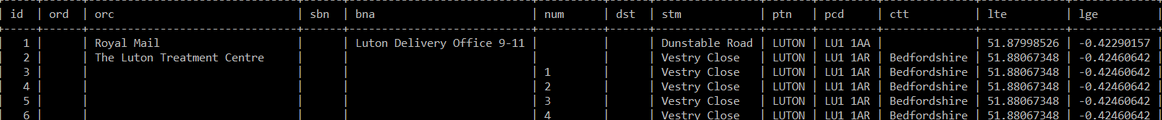
\includegraphics[scale=0.47]{chapter5/parsed1}
\caption{Processed/Parsed Royal Mail PAF Data Set}
\end{figure}

From the original 36 columns of raw data, it is now reduced to a mere 13 columns, as presented in Figure 5.6. The duplicated or unnecessary information and rows are removed from the data set. In this case, information such as flats and sub-houses are taken out, as this is not relevant to the study and will not be used in the visualisation process. Figure 5.6 shows the data before the filtering has been applied. 

\begin{figure}[H]
\centering
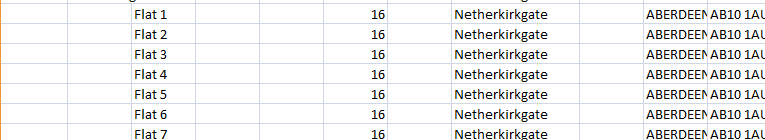
\includegraphics[scale=0.7]{chapter5/flat_filter1}
\caption{Mined / Refined Royal Mail PAF Data Set}
\end{figure}

Through the refinement, the rows above have now been converted into a single row, as illustrated in Figure 5.7. This will make the identification of this area easier and much less cluttered in the final visualisation. The raw data set has repetitive data elements which were filtered at the acquisition and data analysis stage of the information visualisation model. The filtered data is then passed onto the representation layer for visualisation. 

\begin{figure}[H]
\centering
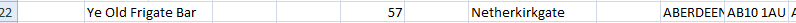
\includegraphics[scale=0.6]{chapter5/flat_filter2}
\caption{Filtered Royal Mail PAF Data Set}
\end{figure}

This process might seem simple and basic, the filter used to apply this process (known as the normalisation and data filter) can be difficult to create and a time consuming process to apply; especially to a data set of this size and complexity. Data mining involves several techniques but the basic premise is that it creates a basic instruction for the computer using a combination of statistics, mathematical analysis and data mining. It starts by shifting the data and applying purely cosmetic changes; for example filtering and removing raw data that is above a certain size or density. This helps remove the information that wasn't relevant or necessary for the desired output. In this experiment, the identified and extracted examples of repetitive postcodes and duplicated rows which are unnecessary was removed. The next section discusses the visualisation model for the acquired data.

\section{Data Representation}

Represent++ is the data representation layer of the proposed visualisation model which allows users to manipulate and understand the data more effectively. Representation of data can have many forms (charts, graphs etc). For this experiment on the UK postcode data, visualisation is done using an interactive map and combine it with data mashup techniques. The data presented to the representation layer is already been processed and analysed in the previous step. The conversion of raw data into a normalised form is then pushed onto the the representation layer where data is visualised with the help of various technologies. The next step in the visualisation plan is utilising the data that has been refined. For this purpose, web maps are the perfect way to display the extracted data, as web maps easily deliver up to date information. If a map is programmed to be generated automatically from a database, it displays new information in real time, without much waiting and further editing. They are also superior to traditional maps, they don't need to be printed, mastered and distributed, are quickly updated and much easier to work with.  A few examples of interactive web mapping in action include:

\begin{itemize}
\item 	A map displaying election results as they are tallied, as soon as they become available from counting.

\item	Maps displaying live traffic updates in almost perfect real time, using data collected by traffic sensor networks. 

\item	A map which shows in detail the current locations of mass transit vehicles (such as busses, trains, ferries or planes). This allows the passengers of the vehicles to  minimize waiting time at stops or stations, and allows to be aware of the delays in service, should there be any. 
\item 	Weather maps used by the media, such as NEXRAD \cite{smith1996intercomparison}
\end{itemize}

Another advantage of using interactive web mapping lies in the cost. The software and hardware used to create map infrastructure for the web is cheap, and web server space and hardware is equally inexpensive, and with many open source tools available for use, it is easy to create professional and fully functional web maps quickly \cite{de2006opengis}.\\

The web maps also give users many more advantages than we perhaps thought of. For example, pushing out and distributing product updates has become a much easier task. This is because web maps distribute data with every single request or load so updates can happen as quickly as a user reloads a page. In more traditional cartography one would need to deal with minor map updates having major ripple effects. If a road name changes or a roundabout is placed, this simple update can be administered in seconds in web maps, but in print it can trigger a reprint, remaster and full redistribution of the media. But one of web maps greatest strengths is also its greatest weaknesses. Because updates are cheaper, easier and faster, it can occur more frequently and even the base product is cheap and quick to create. This is perhaps one of the main reasons many web map's are of astoundingly poor quality; both in symbolisation, content and actual data accuracy. An added bonus for some businesses or organisations interested in this kind of data is that detailed information is now available to discover and combine on a lot of private and personal information of individuals. The details and images of properties and estates of private individuals are now accessible to the general public in high resolution through the web mapping tools. Web maps also allow for complete personalisation. Through the utilisation of user profiles, personal filters, styling and symbolisation anyone can spawn, configure and design their own maps from scratch, providing their chosen platform and mapping system supports personalisation. This personalisation even reaches into the realms of accessibility, and can be used to solve a series of problems. Users can personalise various maps, storing their favourite colours and patterns to identify areas while avoiding colour combinations users can't easily distinguish due to medical or accessibility reasons (e.g. colour blindness) \cite{ware2013information}. Figure 5.8 highlight an interactive map, which was created by processing data through our data mashup system. Using this the Royal Mail postcode data will be visualised. This map shows the United Kingdom as a general space, and separates it into basic geographical locations. 
 
\begin{figure}
\centering
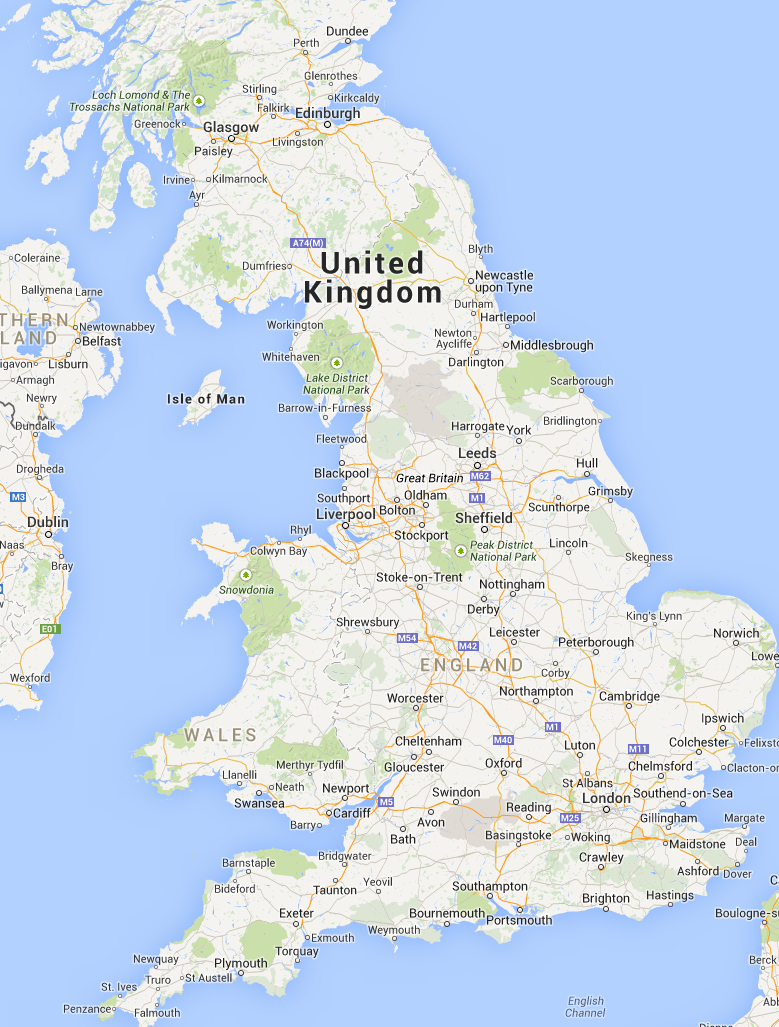
\includegraphics[scale=0.7]{chapter5/web_map1}
\caption{Interactive UK Map Generated}
\end{figure}

Figure 5.9 shows a section of the map segregated by postal regions using the Royal Mail postcode data that have been refined It has been visualised on a fully interactive map, and using web intelligent agents users can read data from the database and feed it back in real time.

\begin{figure}
\centering
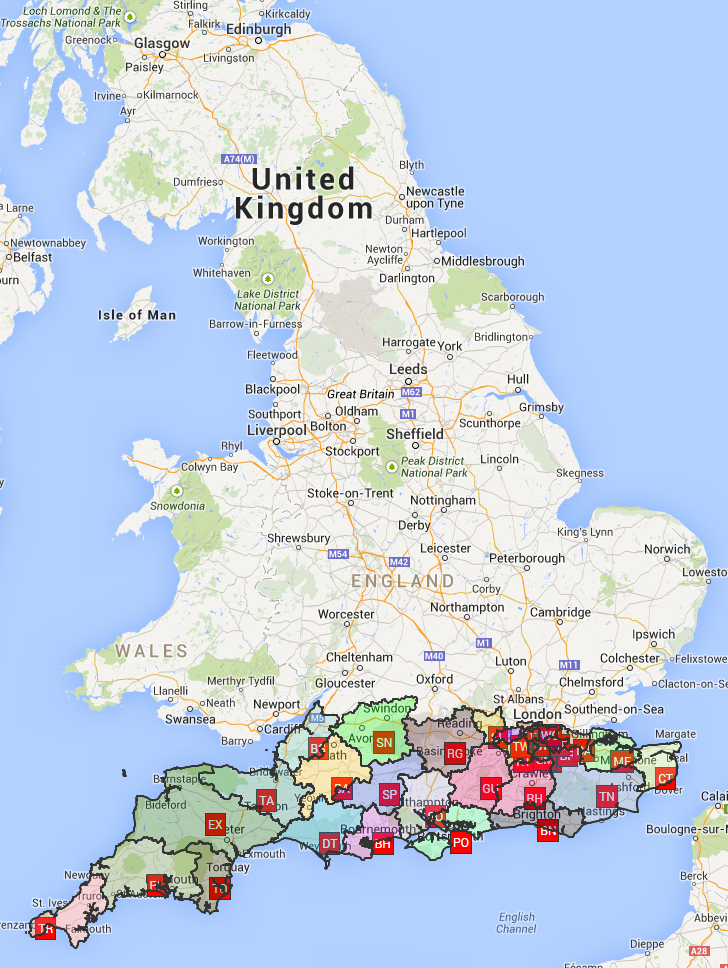
\includegraphics[scale=0.75]{chapter5/web_map2}
\caption{Extracted Postcodes are Visualised with Tags}
\end{figure}	
 
Figure 5.10 demonstrates, data at its next development phase. All of the postcodes are collected from the data set for the entirety of the UK, and have been used to visualise postal boundaries. Red blocks are used to act as tags for each postcode shown, and coloured lines to signify borders. This data can be utilised in several different ways; for example, population density, economic growth, living standards and various other social attributes could be visually portrayed for public and readers. 
 
\begin{figure}
\centering
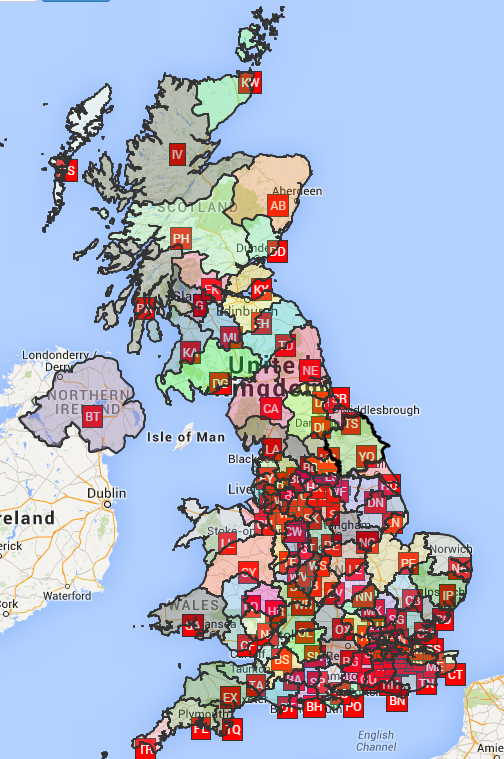
\includegraphics[scale=0.9]{chapter5/web_map3}
\caption{Postcodes are Categorised and Visualised with Animation}
\end{figure}

Once all of the information is collected, users can look closer and dissect it further, Figure 5.11 in the selection is a close up of the Nottingham area. It illustrates a highlighted area in a colour of user's choice for each individual post code area.
 
\begin{figure}
\centering
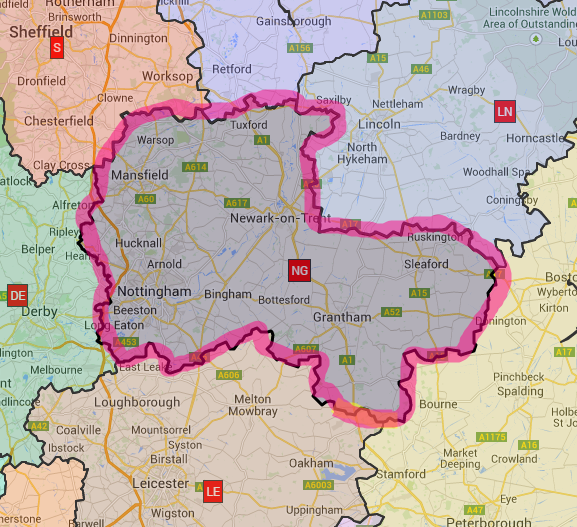
\includegraphics[scale=0.8]{chapter5/web_map4}
\caption{Postcodes Shown with Boundary Markers}
\end{figure} 

Figure 5.12, schools and colleges are shown along with the Royal Mail postcode data illustrated on the map with postcode boundaries. Thus making very easy for the users to understand which colleges or schools fall under what postcodes, these maps are further discussed in chapter 7.

%figure 12
\begin{figure}
\centering
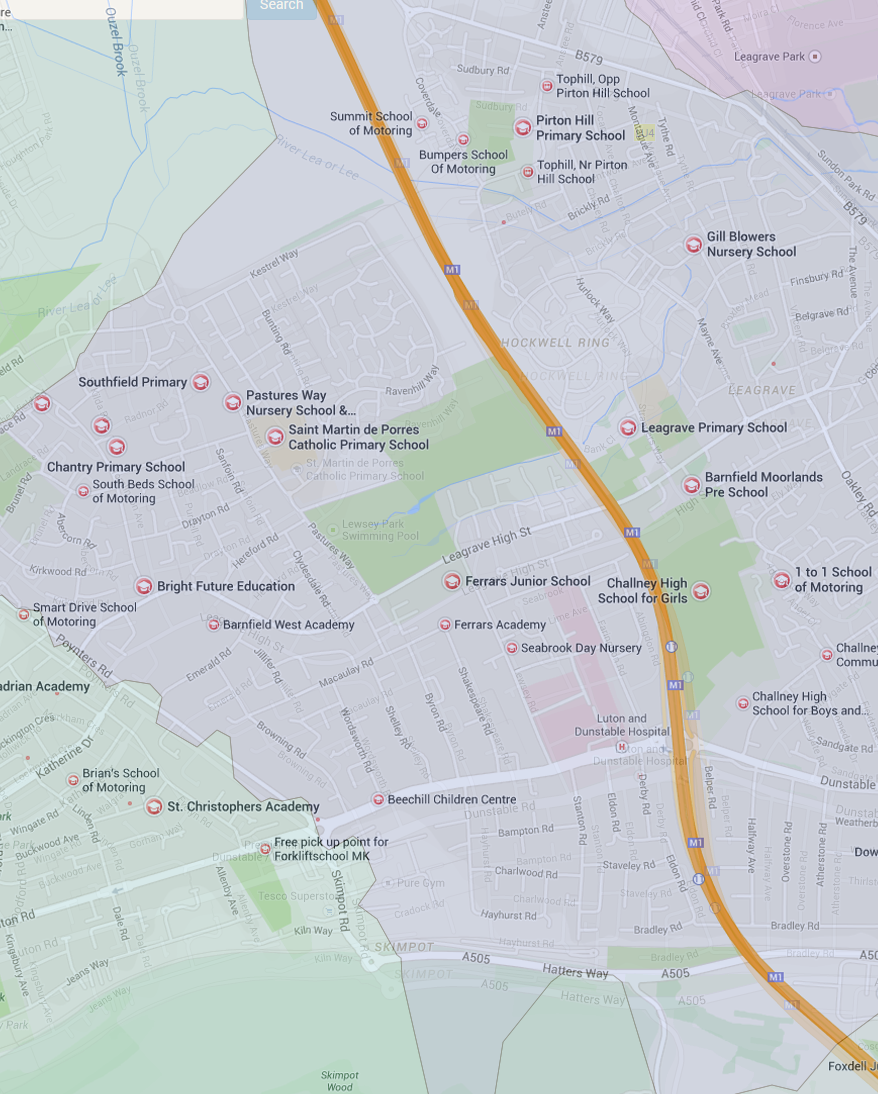
\includegraphics[scale=0.47]{chapter5/schools_map}
\caption{Postcodes Shown with Boundary Markers With Colleges/Schools}
\end{figure} 

The data was retrieved from the database which was initially refined and structured in the acquisition and data analysis layer. This layer have retrieved information from the database through web intelligent(PHP functions) and visualised on an interactive map, where postcodes information is shown in various types. The first or the default screen of the system in this layer shown full UK map with postcode classification and categorisation. The end user can quickly see where a postcode starting with two characters located on what area of the country. The view is further explored through input or zooming in from the user to see further information on a specific area, which then gives additional sub postcode geographic areas distinguished with different colours and surrounded by the boundaries of the postcodes. Sub postcode is additional division of the postcode. The third and final view of the map gives complete list of the postcode in the specified or user selected areas, giving precise information which streets falls under a particular postcode. The postcode map could be an education tool for people from all round the society, with creating knowledge and awareness about UK geography and specially encouraging people to understand complex postcode system with an ease. The next section discuss how the user interact with the data and the web map system.

\section{Interaction }

The next phase of the experiment is about the user and system interaction, which involves adding a new layer onto the interactive map. This new layer of visualisation model acts as a system, and this is utilised to help users gain the ability to interact with the data. This is what transforms the map from a reactive model into an interactive one. Without it, users can't explore the data and gain a deeper understanding. Interacting with data requires digging deeper into the sub levels of the data, finding the hidden gems of information that are not visible at the higher level view. For example, if a user is to select a postcode from those listed in the data or tagged on the map, users can zoom into the interactive map to study it in more detail. When in this view, the user can now see additional sub categories that were not available in the initial view in this case the sub-postcodes that are depicted in Figure 5.13. These are identified with yellow tags, and more information is displayed the further on the map as the user descends further.

\begin{figure}
\centering
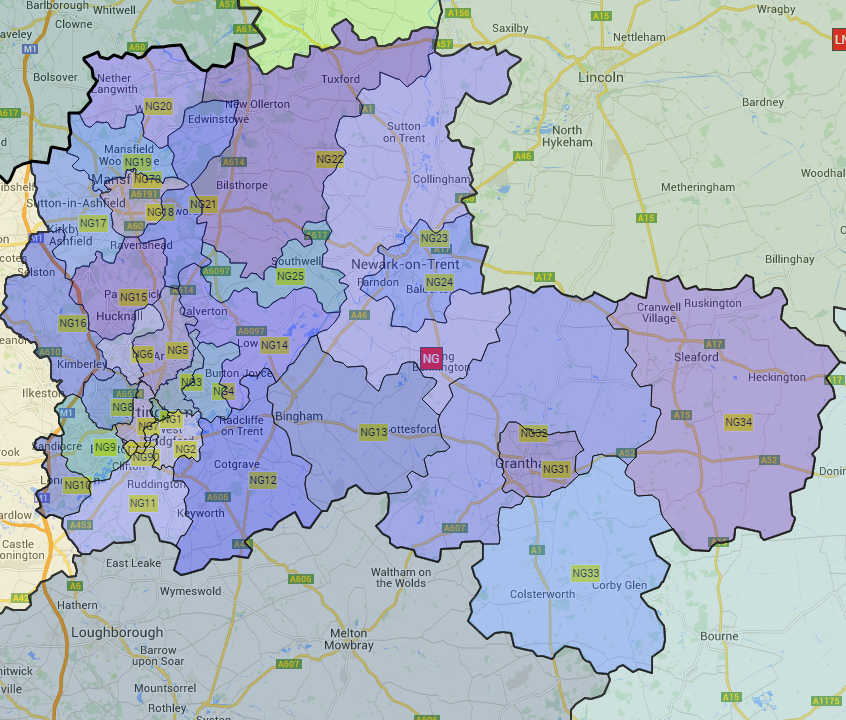
\includegraphics[scale=0.65]{chapter5/web_map5}
\caption{Sub Categorisation of Postcodes Shown with Boundary Markers & Colours}
\end{figure} 

These little sub categories give even more information to the user and the system understands and compensates for that. The system used to create this interactive map is incredibly intelligent, and the new sub categories that are available are now marked with their own tags and boundaries. These are all in different colours with corresponding tags, while still remaining different from the upper levels of distinction. In this new level of interaction, a user can quickly and easily see where NG33 lies on this map. NG33 is sub postcode located in the city of Nottingham as demonstrated in Figure 5.14.

\begin{figure}
\centering
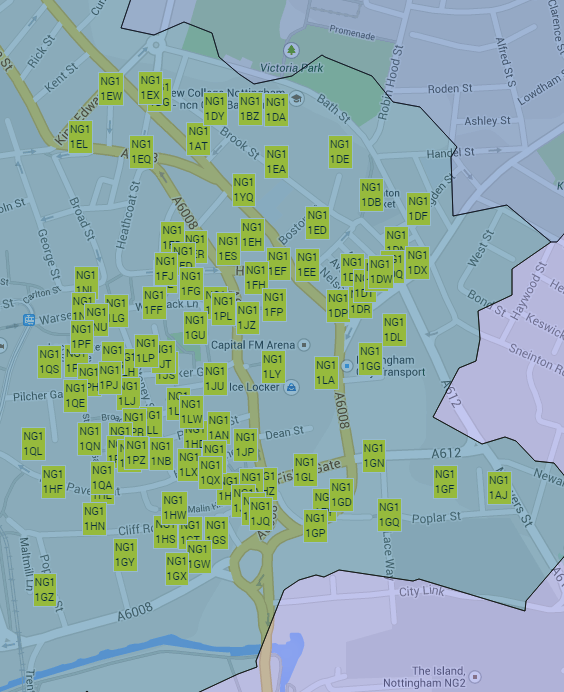
\includegraphics[scale=0.8]{chapter5/web_map6}
\caption{Detailed Postcodes Visualisation with Boundary Markers & Colours}
\end{figure} 

The information could be drilled down further and further, into more detail by continuing to refine the data, searching or interacting with the system. As it is demonstrated above, the further user dig, the more detailed information about the postcode can be shown on the map. It is highlighted clearly where each postcode is located on the map, and if users choose to investigate further they could see the street names belonging to each postcode at each address.

The model has shown the capability of possessing a large, bulky set of data which was quite challenging to understand or manage to having a fully visualised version that is streamlined and easy to read. This has involved many different processes, streamlining, filtration, data mining and parsing before it has arrived at this stage and without those key processes the data would still be almost unusable. This practice can be applied to any form of data set on any subject, and can be used to convert masses of data into simple visualisation forms. By visualising the data in this way, users are able to discern more than one would be able to at face value. The result of the process doesn't have to be a map either there are various other visualisation styles available that can be used to give decision makers key insights about business transactions and customers. These different visualisation styles are highlighted in experiment two. Exporting reports and data storage is discussed in the next section.

\section{History}

The users are given option to export reports into JPEG, GIF, PNG and PDFS. The system produces high resolution images and screen extractions for external usage. The map available to user at the interact++ layer also has the feature to copy link of the generated map along with tags highlighted for points of interest such schools, colleges, churches, mosques or supermarkets. This tool becomes a quality asset for users who are keen to learn UK geography through the postcode perspective or based on the location attributes. The reports and maps are also available to web services which could easily be embedded into any other application. 

\section{Summary}

A complex data set has been processed and analysed and then presented into a visualised form thus exploring data at a different angle. The base data set has been experimented with additional data set for the added value features. The visualisation model and its four stages are explained individually supported by figures and screen shots from the application. In the next chapter, a different type of data set has been analysed. The data set in chapter 6 is a business transactional data set. The same four stages of visualisation are followed data representation and interaction with user. 




 
% Chapter 6

\chapter{Experiment Two - Business Transactional Data} % Main chapter title

\label{Chapter6} % For referencing the chapter elsewhere, use \ref{Chapter1} 

\lhead{Chapter 6. \emph{Experiment Two - Business Transactional Data}} % This is for the header on each page - perhaps a shortened title

%----------------------------------------------------------------------------------------

\section{Introduction}

In the previous chapter, an experiment was undertaken with a large UK geographic postcode data set through the proposed visualisation model. In this chapter, business transactional data set will be analysed through the proposed visualisation model with more complex and even diverse than the previous experiment data set. The data set holds business transactional data from a commercial company for over seven years of trading. This data ranges from sales data to customer feedback, and also includes web based business analytical information. It has been processed by the proposed information visualisation model in order to find any hidden trends within the data, and to explore the analytics for the business, in order to allow for more effective resource utilisation in a real time business environment. The second part of the experiment also have a bespoke tool developed under the same visualisation model for non-enterprise data sets. The two parts are supported by various figures extracted from a live system. 

\section{Acquisition and Data Analysis}

The acquisition and data analysis elements of the information visualisation model are discussed in this section. A transaction can mean different things depending on the context, but in this particular instance a transaction is defined as a sequence of information exchange and related work (such as database updating) that is treated as a unit for the purposes of satisfying a request\cite{williamson1979transaction}. Transactional data can cover finances, logistics or work related data, involve anything from a purchase order and shipping status to employee work hours and insurance costs and claims. Once it has been processed, transactional data is then grouped with its associated master and reference data to create the transactional records. A relevant date and time are added to this, along with the relevant reference data needed for each particular transaction record. Most studies conducted resulting in research and working papers use synthetic data sets in order to produce their control group \cite{axelsson2000generation}. This is normally done using random number generators to help create more data on the fly, and is usually adequate for research conditions into new data analysis techniques \cite{council2005transaction}.

In the first part of this experiment, these large data sets were made available directly to the visualisation system for purely business and data analysis purposes. The data sets which have been obtained for the first part of the experiment consist of several million records, collected from various sections of the existing enterprise systems. The data consists of various different factors and user behaviours, including:

\begin{itemize}
\item Geographical Location
\item IP Address
\item Transaction amount
\item Transactional type
\item Shopping Times
\item Sales Transactions   
\item Staff Behaviour
\item Conversion Figures 
\end{itemize}

The details along with resources such as drivers and vehicle information for transport companies were provided in huge masses of raw data sets for analytical purposes. The proposed information visualisation model process involves various different data analysis techniques, followed by representation (or visualising the data), couples with the interactive layers in the visualisation model. The term enterprise 2.0 within an organisation is used, it is usually referring to an environment of the business where data is available in a normalised form and accessed through web services and APIs. The enterprise environment is a very modern idea, and has been designed with a multi-user and multi-developer base in mind. It's because of this new, modern idea that the data analysis can be processed in a real time environment but before diving into full data analysis in an enterprise environment, the applications are highlighted below. Like any other modern application, an enterprise application has to be reliable, perform well, provide intuitive and effective user interface and live up to high levels of data usage without struggling \cite{fowler2002patterns}. Enterprise application is typically characterised by these three attributes:

\begin{itemize}
\item 	Multi-component Enterprise:  Where applications are rarely utilised for smaller amounts of data. When it is developed into a multi-user, multi-developer machine, it becomes a sophisticated multi-component application that can handle and manipulate massive amount of data while using streams of built in extensive parallel processing, resources distributed by various networks and very complex logic with ease. Such applications can be deployed across multiple platforms and inter-operate with a variety of different other applications, and it is an incredibly long lived solutions. Accounting, enterprise assets management and database management system are some examples of multi-component applications.

\item	Business Oriented: The specific purpose of enterprise applications is to meet very specific business requirements. The application encodes business policies, processes, rules and entities, and is developed within the business organisation to suit their needs. The application is then deployed in a variety of manners, all of which are responsive to the business needs. Reporting, resource management, business performance and business intelligence are some examples of such applications.

\item	Mission Critical: For a lot of businesses, enterprise applications fulfil a mission critical role. For this reason, an enterprise application must be able to stand up to a lot of pressure, and robust enough to endure constant operations. It must also be flexible to allow for extreme scalability and instant deployment while being accessible enough to allow for effective maintenance, monitoring and administration. Critical infrastructure and crisis management are a couple of areas where mission critical applications are utilised.

\end{itemize}

The combination of these qualities understandably makes the task of developing an enterprise application an incredibly daunting and challenging. This made even more difficult by the new trend towards businesses making rapidly increasing demands of their applications. This is supported by the rapid improvement of computer hardware and software within the business world, combined with a quickening global economic competition. This competition and the opportunities it spawns, have created a unique environment in which business systems are forced to respond at faster and faster speed in order to deliver unparallelled levels of performance and service. As these demands continue to rise, the developers of the applications are pushed to automate more and more of their business applications, to build their software even faster - enabling it to serve more and more users and process a rapidly growing mass of data. Putting all of these challenges aside, the sheer power, complexity and rapid change of technology used in the building of these corporate solutions make simple and efficient development of applications even more difficult.

The process of designing and developing an enterprise application is a complex one, and in order understand the process, some of the requirements are listed below.

\begin{itemize}
\item 	The business goals.
\item	How soon the application must be delivered.
\item	It's budget.
\item	How many people will develop, test and maintain the application.
\item	How many concurrent users the application will need to support.
\item	The importance of performance in the application and the ease of use.
\item	The hardware it needs to run on.
\item	Where it will be deployed.
\item	What security is required for this business.
\item	How long the application will be used for.
\end{itemize}

To understand relationship between such complex and conflicting requirements that requires a systematic approach. It needs to simplify the model and reduce the levels of complexity in order to provide an organised way to design and build applications, and ones that chart the optimum course among the many requirements of the applications. That process is demonstrated in Figure 3.3. At the root of any visualisation process lies in data analysis. Using the proposed methodology, the system will be able to establish what environment the visualisation request originated in - an Enterprise 2.0 environment or a non-enterprise environment. The origin determination will decide how the request is processed. If the request originated in an enterprise environment then the proposed system will already be aware of the data structure, and will have direct access to the data sets through web services and API's. 

The mashup application will also be able to understand the data structure, and therefore will be able to directly access information as and when it is needed for the visualisation process. This system will have direct and multiple connections with data sources in real time as the data sources change and alter. The proposed system application will be updated and new data acquired from the source, as shown in Figure 3.3. The benefits of processing data in a familiar environment is that the first four main stages of data analysis (acquire, parse, filter and mine) can all be achieved through basic API's and web services or web intelligent agents(PHP functions). For example, if a particular application requires sales figures for it's visualisation, a mashup system combined with web intelligent agents could search for and access the sales figures through API's in the familiar XML format before passing it on to the system as another layer for the visualisation process. Any information the system required could be easily and directly accessed, and that's the key benefit and essential for any system to work within a known environment.

Data acquisition is a process is executed through web intelligent agents and the instructions for this usually come from a business supportive model. This model is designed by management within the business, and is used to initiate and process certain tasks. These tasks are made up of clear instructions to the system, including what information needs to be identified and fetched for analysis. The visualisation model describes the rationale and process of how the business will create, deliver and captures value within an economic, social, cultural or other context. The process of constructing a business model is an essential part of the business strategy. and within the model there is a business process or method, comprised of a collection of related and structured activities, all of which produce specific services or products to serve a particular goal for customers. This often easily visualised as a flow chart, with a sequence of activities with interwoven decision points, or when using a process matrix, a sequence of activities with relevant rules all based on data within this process. There are generally three types of business processes, all of which are detailed below \cite{van2003business}.

\begin{itemize}
\item 	Management processes: These are the processes that govern the operation of a specific system. A typical management process includes corporate governance and strategic management.

\item	Operational processes: These are processes that constitute the core business model and help create the primary value stream within the business offering. For example, taking orders from customers, or opening a bank account within a branch are both operational procedures.

\item	Supporting processes: These supporting processes support the core processes within the business. Examples of this include the accounting and human resource management.
\end{itemize}

Every business process starts with a mission and ends with the achievement of that business objective. A process oriented business can break down the barriers of structural departments, and do their best to avoid any functional silos. A business process can be easily separated into several different sub-processes, each of which has its own attributes and properties. They also contribute their individual talents to achieving the collective goal, or super-process. To analyse the business processes of an organisation would typically start with mapping out the processes and sub-processes right down to the activity level \cite{aguilar2004business}. The parsing of data is not required in this case - as the information is already in a known structure within the business. As an example, the database table is illustrated in Figure 6.1. The data for this table has been acquired from an enterprise environment where the data about bookings is stored. There are approximately 74 attributes in the table, equating to 74 columns within a spreadsheet format. Each of the 74 attributes represent different information about different bookings. The data set contains millions of records of various business attributes. For example, customers, bookings, resource, staff and assets information are available in the data set.\\

\begin{figure}[H]
\centering
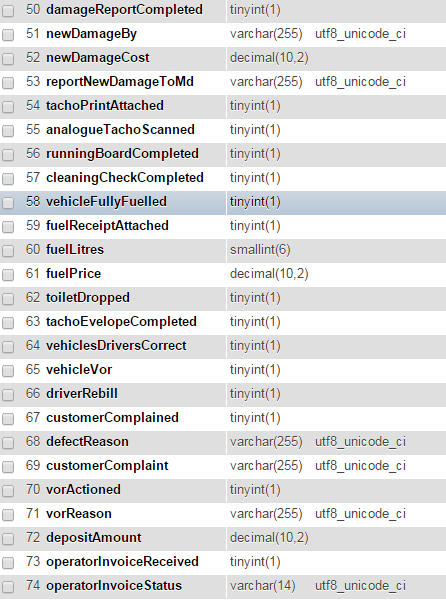
\includegraphics[scale=0.8]{chapter6/booking_table_3}
\caption{Booking Table from Database Overview}
\end{figure}

In this situation, the refining and filtration stages of data analysis are not required, as the business support models know exactly which fields within the data sets need to be retrieved for analysis purposes. The database table shown in Figure 6.1 helps to clarify the nature of the attributes. The system has the ability to transfer data into simple visual content. For example, if the system is asked a question (or query initiated) by the manager through a business supportive model (in this case, how much fuel does a booking cost?), an analysis model will read that command and will only retrieve information which is related to the fuel from that database. In this instance, the system will fetch the attribute 61 as shown in Figure 6.1 labelled as Fuel Price. The visualisation model will then be able to use and process that information, and turn it into a visualisation output to allow the decision makers to see and understand it easily. The process is simple in an enterprise environment, in a non-enterprise environment it needs to be handled differently. If the data sets are not accessible through traditional means such as API's, or if it is in an unknown structure, the mashup application must then request mining tasks. The acquisition and data analysis process for non-enterprise data is handled through a separate and dedicated information visualisation tool created on the same principle of the proposed information visualisation model called Visualixer. The Visualixer then process raw data and remove, filter and then parse and mine information into the MySQL database. The data is then available to the data representation layer for visualising. The full system features of Visualixer are explained below, along with a brief summary of the more important sections and features.

\subsection{The Visualixer System for Non-enterprise Data Sets}

The Visualixer system has been specifically designed to deal with data that is in a non-enterprise origin. Usually data extracted from this kind of environment is taken from a complex system and this means that the data itself lacks any specific meaning and is overly complex to analyse. That is the reason for creating a visualisation tool for this type of data, to allow users to overcome complications and access meaningful data and developed this by adapting the same theoretical model as used in the chapter 3. In the next section, the review of the menu structure within the Visualixer system to explain the processes and functions.

\subsection{System Features}

Following are the main system features:

\begin{itemize}
\item Data Import:

Import data is one of the most prominent tools within the menu system and one that helps users to easily and effectively import their data in raw format into the tool. Once the raw data has been imported it can be formatted into various data types (.CSV Mac-In tosh, .CSV MS-DOS, XML data, Excel template etc) and fed into the visualisation tools. The data file that needs to be visualised can be simply and easily uploaded into the system by selecting the appropriate file and clicking upload.

\item File Management:

Using this menu, users can upload files directly into their account. Once these are uploaded the files are automatically stored within their account for later use. This function enables the user to select, delete, edit and visualise data at any time. This feature is a fantastic facility for user, businesses and organisations to compare and analyse their results in various time zones at their own leisure. For example, a coach company can not only clearly visualise their data, but also analyse and understand the data, the business and the performance of various employees in a single click. 

\item Business Intelligence:

The main purpose of the information retrieval is to allow for the effective mapping of business intelligence for the organisation. Visualixer can help here in two ways; first it is able to retrieve the information from its raw source, and then it is able to provide comprehensive intelligence to the organisation to help better understand their business. Once it has been processed, the visualised data can then be presented to the relevant management within the organisation, and help the business to visualise their structure and information perfectly. Within the model there are many different statistical charts that can be utilised to present the visualised data collected from the source. 

As explained previously, the primary goal of any data visualisation tool is to optimise the data and help decision makers to make more informed and accurate decisions by providing with details such as deeper knowledge of their business, customers, workers and seasonal changes. All of this aids in the building of a clear and successful strategy for growth for the organisation.
\end{itemize}

\subsection{Visualixer Operational Overview}

Using the import data menu discussed above, the users are helped with the Load and Transfer functions within the business intelligence stack of the system. The system overview page comes pre-loaded with the features, each of which can be used by any member of management to move the analysis forward. These are basic functions that are very easy to use the select file and upload. These functions are very similar to the method used to attach a file to an email and hitting send. The system overview page is what lets the client easily retrieve data and feed it into the Visualixer system interface.

My Files menu, which shows the user all of the files uploaded in the system. Registered users have the ability to upload and edit files.  The system has successfully stored a history of the data for later review, and displayed this visually within the menu. This is a new feature that has been specifically designed for the Visualixer systems allowing the storage and backup of data history along with the ability to edit, delete or visualise the stored data at the touch of a button making the job of key decision makers easier.\\

The edit function within this menu is particularly interesting, and one that warrants further exploration. Any queries for the system can be solved and subsequently edited by the user regardless of any knowledge in writing queries for computer programmes and databases. This function drastically improves the accessibility of the programme, and allows users freedom to play with the system and with the data content. There is a delete option, which makes it easy to remove data with a single click without going through a multitude of complex procedures. The data visualisations and the internal tables are then automatically updated after the data is deleted, allowing real time updates.\\

This section has discussed and explained two different of environments in acquiring and analysis of complex data sets. The data analysis model is extensively defined supported by actual system. The processed information is then passed on the data representation model where the data is reproduced in a visualised form. 

\section{Data Representation}

The represent++ layer handles all aspects of data representation which involve converting data into a visualised form. The data is passed onto this layer from acquisition and data analysis layer discussed in the previous section. 

In this section, the data representation aspects are discussed with example extracted from a live system for the above explained data set which includes business transactional data.

The graph shown in Figure 6.2 is the perfect example of a traditional bar chart. It includes 2 axes, an X axis to denote the price that is achieved in sales by the employees, and a Y axis to show the number of employees in the organisation. There is then a visualised rectangular bar, which has values proportional to the value of the employees cross referenced with their number. 
% Figure 6.2
\begin{figure}[H]
\centering
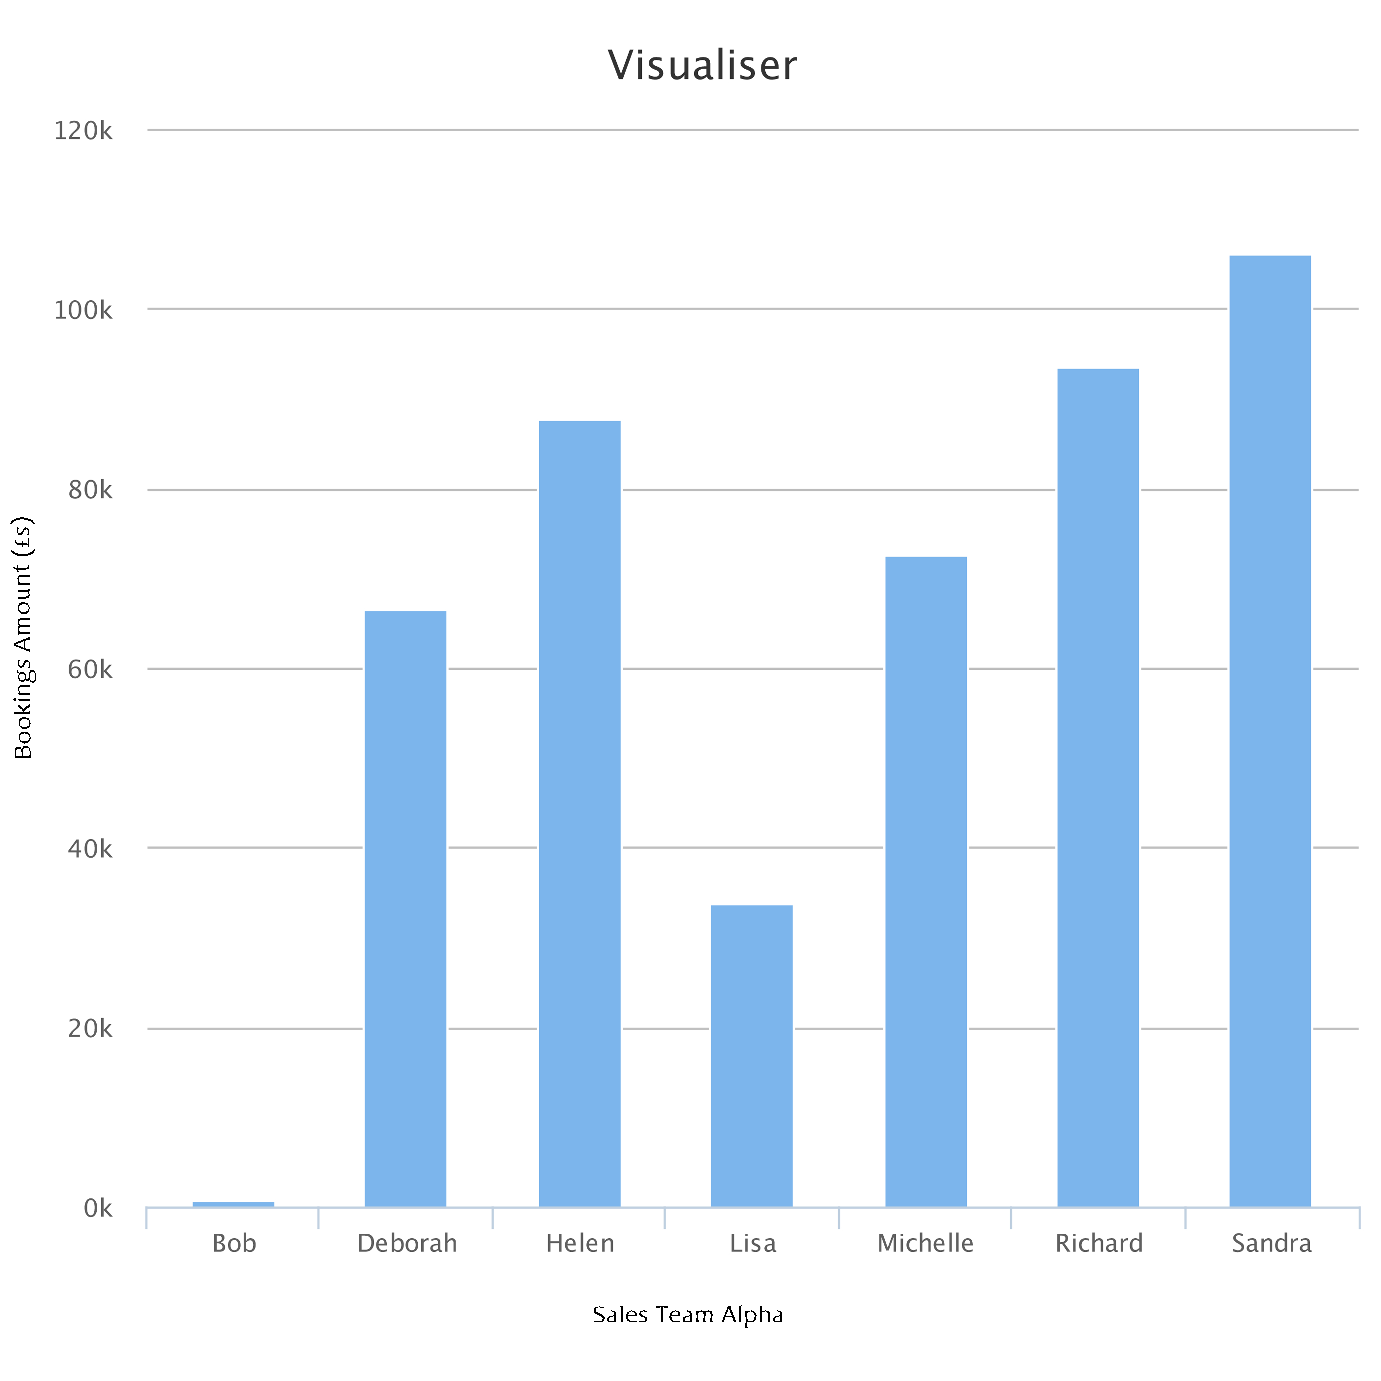
\includegraphics[scale=0.5]{chapter6/bar_chart}
\caption{Classic Bar Chart Data Visualisation}
\end{figure}

This chart is an easy and simple way to visualise the targets achieved by the employees against each individual name - and was used as the basis for a performance review. These are also helpful for drawing comparisons between employees and their performance, identifying trends in performance and combinations that produce better results within any organisation.

The more complex data visualisation are achieved through these simple form of representation with combination of more than one charts which helps in analysing data from different perspective. The data acquired from the previous layer, usually present data to the visualising engine in the form of an array. The array in listing 6 shows part of more complex data set.

\begin{listing}[ht]
\begin{minted}
[
frame=lines,
framesep=2mm,
baselinestretch=1.2,
bgcolor=LightGray,
fontsize=\footnotesize,
linenos
]
{python}


['Years',    'Web', 'Affiliates', 'In-Store',  'Door',  'Phone'],
['2008/09',   165,      938,       522,         998,     450],
['2009/10',   135,      1120,      599,         1268,    288],
['2010/11',    157,     1167,      587,         807,      397],
['2011/12',   139,      1110,      615,         968,      215],
['2012/13',    136,     691,       629,         1026,     366] ]);

\end{minted}
\caption{PAF Raw Data set Conversion Sample Code}
\end{listing}

The data is in an accessible form (extracted sample as above), this needs to be visualised. To do this a combination of tools including charts, API's, external Java Script visualisation systems and other pre-existing visualisation tools which are accessible to the system via the mashup application are utilised, the more complex examples such as transactional tagging and linked data visualisation codes are written for this research as the same output was not possible with the pre-existing technologies. \\

The concept behind the proposed research model is to represent complex data attributes in the simplest of visualised form. The visualised data is demonstrated in an area chart using one of the views and output systems in Figure 6.3. This visualisation practice can be considered as a non-coordinated, or single visualisation approach, and is commonly used within the field of information visualisation by various applications.\\

% Figure 6.3
\begin{figure}[H]
\centering
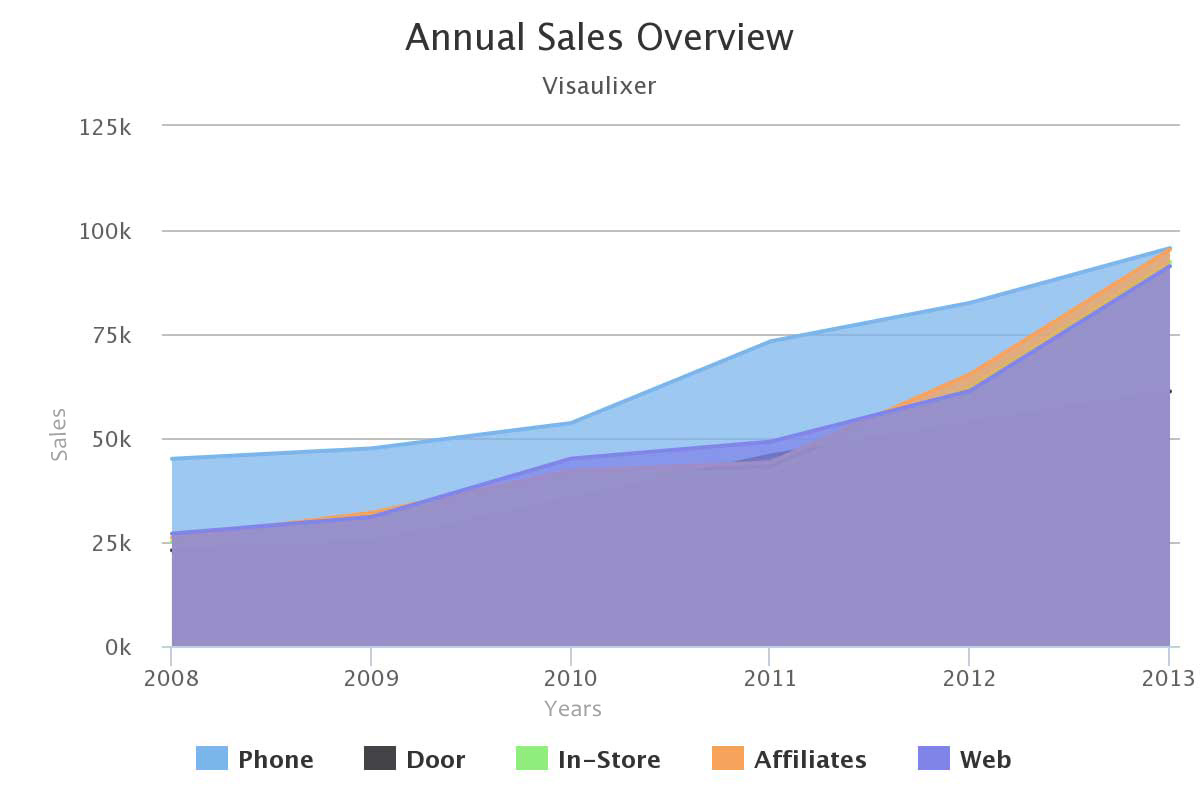
\includegraphics[scale=0.3]{chapter6/areachart}
\caption{Data Visualisation Through Area Graphs}
\end{figure}

This is just one visualisation layout, there are many different types available to end users, increasing the effectiveness of the interface layer and user interactivity, thus allowing it to function more smoothly. In the system there are many visualisation styles, all of which are available at the mashup application customisation layer, or through widget creation allowing users to create a section for each and every data set. 

This technique is often referred to as multi-coordinate visualisation, and is fast becoming the most popular and effective approach when decision makers need in depth information. This is because it is so flexible, versatile and fast; a business transaction picture can be drawn up from the data stored within the system in seconds, allowing decision makers to analyse data and cross examine various different aspects of the data in a single session. Figure 6.4 shows an example of a multi-coordinate visualisation. These simple data representation is interactive and provide more indepth analysis to users. Interactive graphs are not available in programs like Microsoft Excel. 

\begin{figure}[H]
\centering
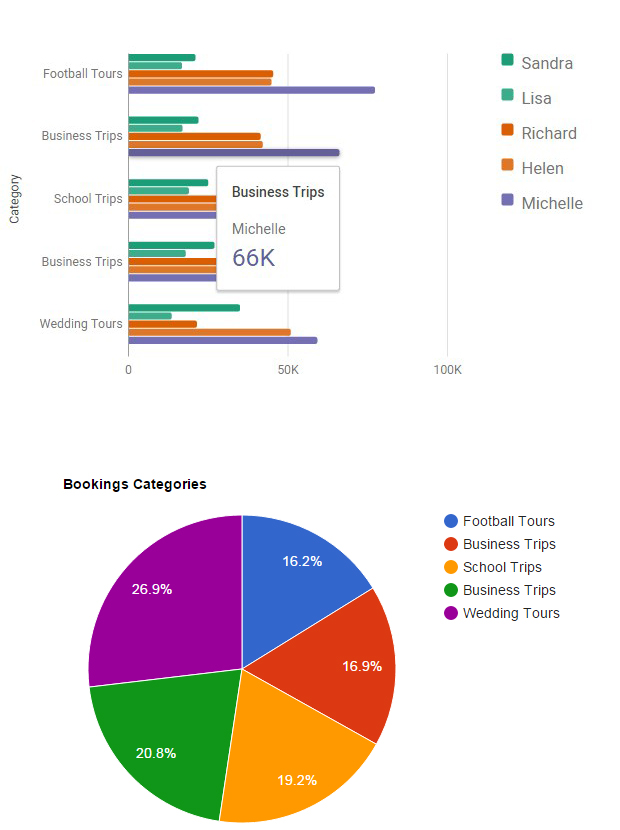
\includegraphics[scale=0.6]{chapter6/multicoordinatenew1}
\caption{Multi-coordinate Data Visualisation}
\end{figure}
%------------------------------------------------------
% Transactional Tagging Starts
%------------------------------------------------------

In information systems, tagging is considered non-hierarchical terms assigned to a particular action or sub data elements. Tags are usually added to digital media such as images, videos, audios or computer files. Tags are also very popular in social media websites such as Facebook. It is also some time known as folksonomy \cite{o2009web}. However, it is popularised with the introduction of user generated content in Web 2.0. Tagging helps with data classification and categorisation. Similar approach for the acquisition and data analysis layer in the visualisation model proposed in this research. Its a novel contribution to data analysis field specially to transactional data. The web intelligent explore relations between data elements and the repositories are then retrieved for the data representation layer. The end user at the enterprise environment is also given the ability to tag information. Thus a two-way tagging approach adapted by the system which helps in validating transactions before any analysis is done. Transactional tagging also helps in visualising multiple dimensional data as many attributes could be explored within one visual graph. Figure 6.5 shows an image extracted from the system visualising sample data from the transactional data set.\\
% Figure 6.5
\begin{figure}[H]
\centering
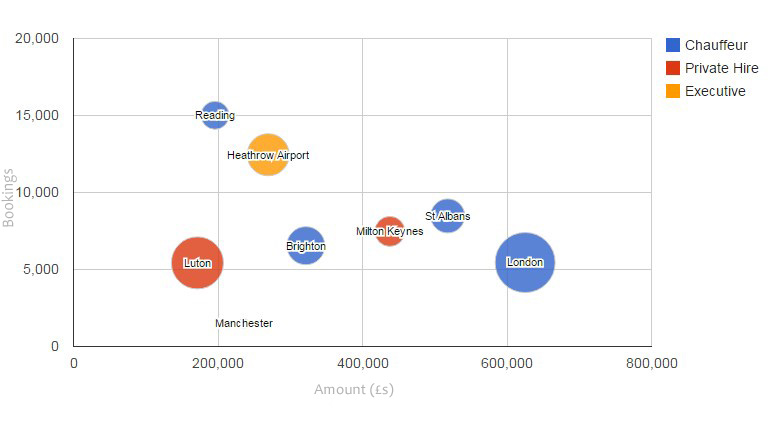
\includegraphics[scale=0.5]{chapter6/Linked_data/transactional1}
\caption{Transactional Data Tagging Visualisation}
\end{figure}

The data which has been visualised is from the bookings table in the transactional data set used in this experiment. Multi-coordinate visualisation has the ability to visualise diverse data and helping users in exploring data trends. For example, in Figure 6.6 various bookings types are highlighted including transactions channels such as web sales, email sales, BDM (Business Development) and phone sales. The same data is further visualised showing which resources (vehicles) were allocated to different categories. Kelly and Klassy were used with orders taken over the phone. Dympa, Becky and Valarie vehicles were used for orders taken through web channels. This kind of data analysis helps decision makers to optimise resource management and revenue streams.

\begin{figure}[H]
\centering
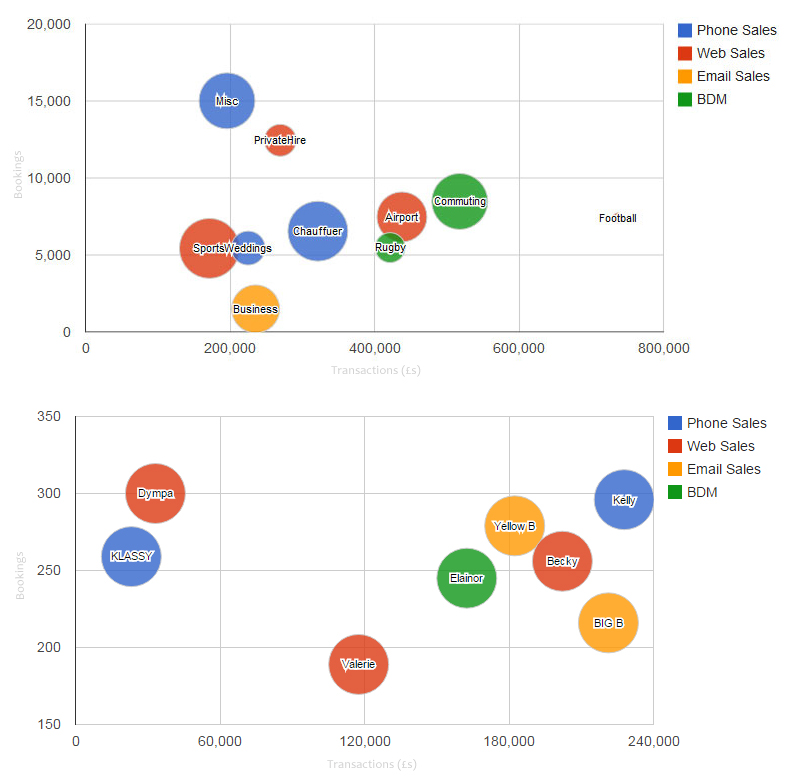
\includegraphics[scale=0.5]{chapter6/Linked_data/multi-tagging}
\caption{Tagged Bookings in Multi-coordinate Visualisation}
\end{figure}

Figure 6.6 demonstrates tagged data in multi-coordinate visualisation form - making it very easy for the end user to cross examine information. The same principle could be applied to any data where multi-attribute data visualised for more in depth analysis and insights.

%-------------------------------------
% Transactional Tagging Ends
%--------------------------------------

%------------------------------------
% Link Data Starts 
%------------------------------------

The Semantic Web is the combination of different types of data elements combined together forming semitic data — the data could be elements of online orders, bookings, articles, financial data, governmental data and available in so many other forms and formats. However, for the linked data phenomenon, it is very critical to have the huge amount of data on the Web available in a standard format, accessible and retrievable by the web tools and applications \cite{bizer2009linked}. The same concept could be applied to transactional data sets or any other data set available to computer systems for analysis purposes. The data should be transformed or made available in a semantic or a standard format where data relations are explored and discovered. The linked data approach has been adapted to find relations and furthermore, visualise those relationship making it easy for the users to analyse complex data sets. An identical approach as that to linked data is applied to different data sets and then the data relations are visualised as a sub set of the main visualisation problem. The following examples will highlight the technique and usage of the linked data visualisation.

% Figure 6.7
\begin{figure}
\centering
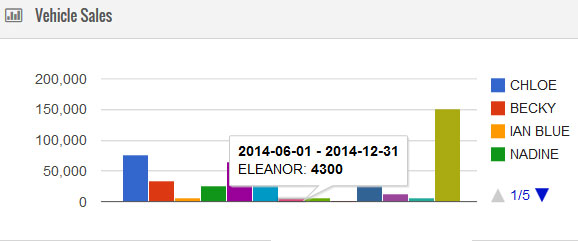
\includegraphics[scale=0.6]{chapter6/Linked_data/vehicles}
\caption{Bar Chart for Linked Data Visualisation}
\end{figure}

The visualisation process is taken place at the same time with other elements of data set. For this exercise, data from the commercial data set has been used. The extracted data shows vehicle sales values in Figure 6.7 for a specified date range. The bar shows each vehicle sales values, upon clicking on a vehicle bar, the locations of the sales are highlighted on an interactive map for the selected vehicle as shown in Figure 8. At the same time, another multi-coordinate chart is generated and showing tagged bookings for the same selected vehicle.

\begin{figure}
\centering
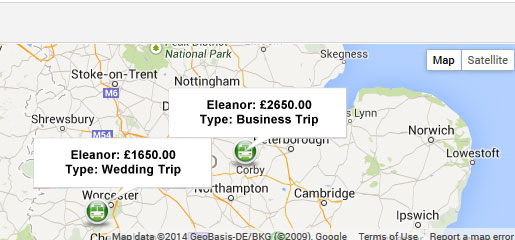
\includegraphics[scale=0.8]{chapter6/Linked_data/geo}
\caption{Live Map for Linked Data Visualisation}
\end{figure}

% Figure 6.9
\begin{figure}
\centering
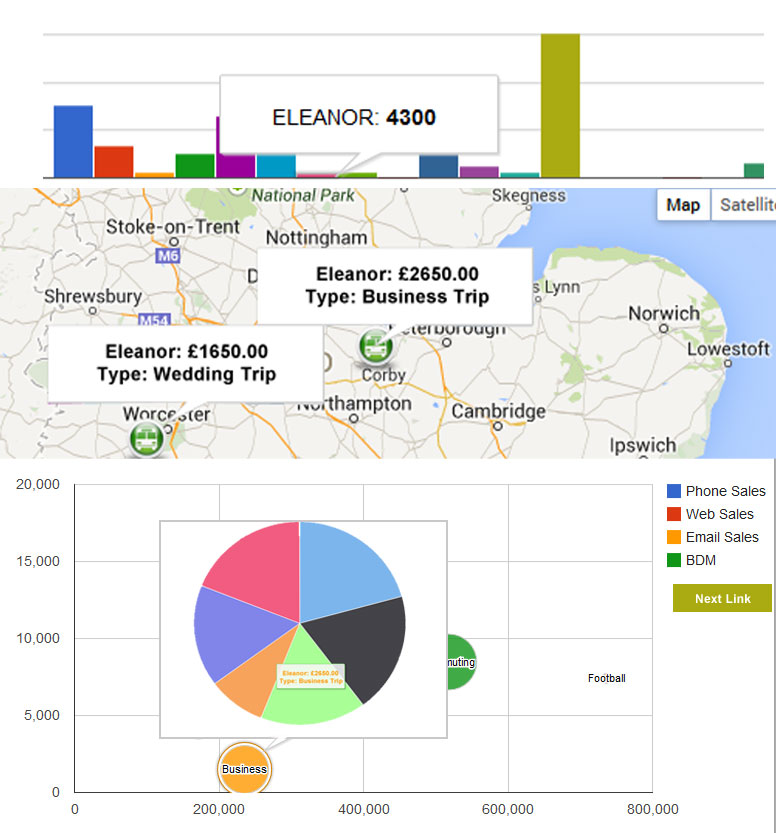
\includegraphics[scale=0.47]{chapter6/Linked_data/part1}
\caption{Multi-attribute and Multi-Coordinate Linked Data Visualisation}
\end{figure}

Figure 6.9 highlights, data element relation in a visualised form. The first part in the image shows some of the vehicles and while clicking on a particular vehicle, in this instance Eleanor, shows two additional charts. The second chart shows information about booking location on a live and interactive map. The third chart shows tagged bookings medium and industry related to this particular vehicle. If the tagged medium and industry are more than one, more information is shown on clicking on the next button, which then produces visualisation of next related data elements as illustrated in Figure 6.10.

\begin{figure}
\centering
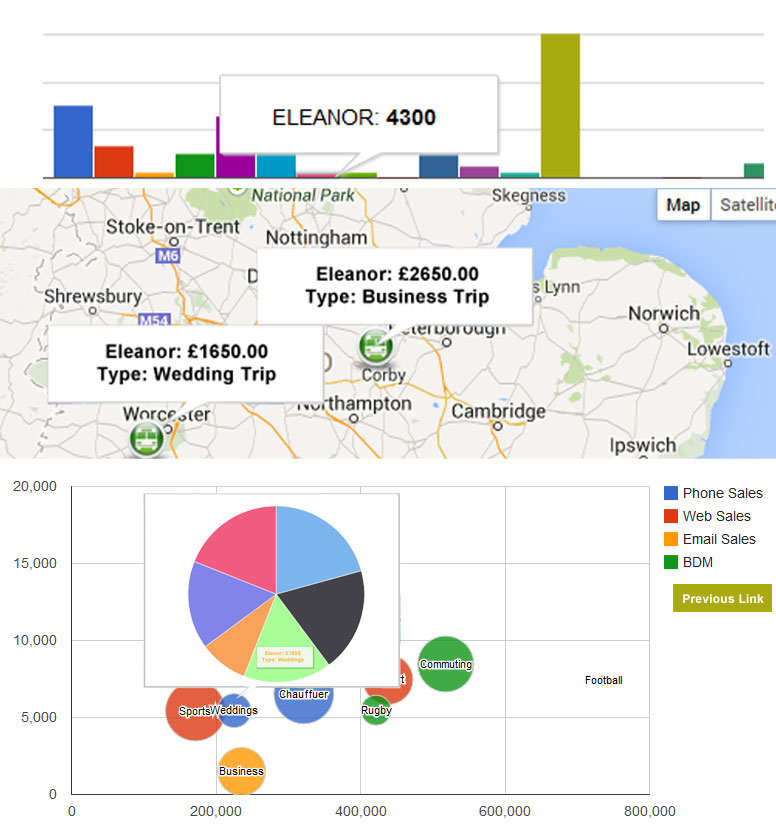
\includegraphics[scale=0.5]{chapter6/Linked_data/part2}
\caption{More Insights Based Linked Data Visualisation}
\end{figure}

The linked data visualisation is a novel contribution in information visualisation. The model first explores relationships within the data sets as demonstrated above and then visualise the information for end user providing ease of understanding and decision making on a particular asset or resource. The linked data visualisation concept is further discussed in the next chapter with a different set of experiment and data types.

%---------------------------------
% Linked Data Ends
%---------------------------------
The Visaulixer tool, designed and developed for the information visualisation model will come into action where data sets are not in normalised or structural form, in other words data sets are in non-enterprise environment. The data import features of the system are explained in the previous acquisition and data analysis section in this chapter. There are various examples of graphs generated by the Visualixer tool at the data representation layer. In the next section, the system interaction features will be highlighted and discussed for business transactional data sets.

\section{Interactivity}

The two important aspect of the system are discussed, as how users interact with the application and the application interaction with the data and the data representation layer. The fundamental aspect is accepting input from a user. Interactive computer systems are functions and programs which allow users to enter data or instruction to the application through interfaces. The applications respond to user requests through these interfaces by providing what the users want to see or expect from the system. Computer programs or devices (in response to a user's action or request) presents choices (paths) depending on where in the program the user has initiated the action. Using these choices, the user can control or change the action of the device or outcome of a game or program. Interactivity is key element in the proposed information visualisation system. The users are given option to interact with visualised content. Furthermore, ability to export information at the interact++ layer. 

In the proposed system, the user has the unique ability to tweak the input or change the data questions, and the system, the intelligent design enable it to accept the changes easily (no matter how challenging) and alter the outcomes, producing output based on the users instructions. All of these various outputs are in the form of interactive charts and graphs of data, which are quickly processed by the proposed system without any problems. With the addition of interactive graphs into the mix, application is able to give additional information which is not always available or visible on the static graphs produced, but nonetheless connected or associated with an event. With interactive graphs, such events are just a mouse click (or hover) away and these graphs will generate more data and information for the analysis purposes. The interactive aspect of the system are utilised in Figure 6.11, the user is given an option to click on area of interest to explore more in-depth information.\\ 

% Figure 6.11
\begin{figure}[H]
\centering
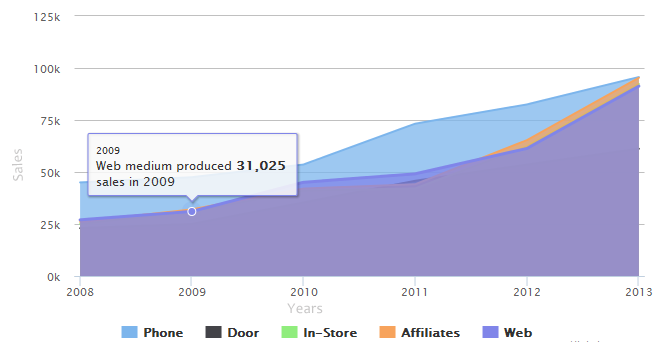
\includegraphics[scale=0.6]{chapter6/mouseover}
\caption{Graph Interaction on Hover}
\end{figure}

These new graphs have another unique ability, it can be used to drill down further into the data; revealing more detailed analysis and allowing us to view non-aggregated visualised information. The interactive layer also allows to zoom-in and zoom out on specific features available in various graphs, and this just adds to the power of this new technology. The interactivity of the graphs is a key feature in helping to achieve a much greater and deeper understanding of the most complex data elements, without the headache of manual analysis. The user have been given the ability to pick and choose different types of data for further analysis, if the user want to see or compare phone orders, it could be achieved with only disabling rest of the elements of the graph as illustrated in Figure 6.12.

%Figure 6.12
\begin{figure}[H]
\centering
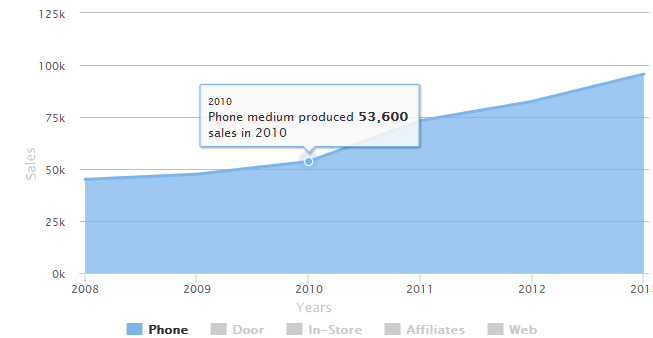
\includegraphics[scale=0.6]{chapter6/mouseover2}
\caption{Selection Option for In-depth Analysis}
\end{figure}

In addition to all of the above, there are also extras that can be added to the interactive graphs to improve their effectiveness and reveal yet more information for comprehensive analysis. There are various data filters which can be applied to the interact++ layer, and these filters have various functions within the layer. The data set has been visualised in its totality. For example, if a system has visualised the booking information for the period of a single month, this could be filtered into a date range that spans two months, depending on the date range used, or even reduced to one day.  The filters can be applied to understand the data more clearly, or to answer a particular data question the user might have. For example, a member of management might want to know how many bookings the sales team have taken in a week, a month or in a single day as in Figure 6.13.

% Figure 6.13
\begin{figure}[H]
\centering
\includegraphics[scale=0.5]{chapter6/salesfiguresdaterange}
\caption{Data Analysis at Interact++ Layer}
\end{figure}

There are filters that can be applied to help the user to determine where this information lies, access it and bring it forward. The filters applied could also be more unique in nature, applied to unique data elements, for example to filter by staff members. This would help answer the query, how many bookings did staff member X generate in one week, or one month? These unique and incredibly useful interactive filters are simply instructions by the users, to display or retrieve information that users have shown an interest in. Interactive presentation is now the focal point of the proposed system, as this technique leads to deeper knowledge and understanding, as well as unearthing hidden trends and patterns about the data sets.

\section{History}

Data graphs which have been generated at the interactive layer also have an extra feature where data can be exported into a specific format such as PDF, JPEG, GIF or even other types of charts and graphs when requested. The history layer within the program allows the user to store generated graphs and charts, and make them accessible to other users upon request. This history element is particularly effective for the comparison or charts and graphs at a later stage; perhaps to review progress or look back on statistics to make judgements on new business strategies.

\section{Summary}

In this chapter, the visualisation model was tested with huge business transactional data set. The enterprise and non-enterprise scenarios are discussed based on how data is acquired and analysed in both of these environments. The data sets where data was not in normalised source, Visualixer data analysis model was presented to support the visualisation process. The data representation layer was then supported with various graphs and charts generated by the system. The user interaction with the system explained and evidence provided with screen shots from the application. The system ability to store information in various formats are discussed in the final section of the chapter. 

Linked data visualisation is introduced and tested with transactional data set. The transactional tagging also explained with the same data set. Multi-attribute and multi-coordinate visualisation techniques are demonstrated with various charts in this chapter. In the next chapter, further discussion of the two experiments is undertaken. The visualisation model and its outcomes are compared with existing tools and technologies. 
% Chapter 6

\chapter{Further Experimentation and Comparative Analysis} % Main chapter title

\label{Chapter7} % For referencing the chapter elsewhere, use \ref{Chapter1} 

\lhead{Chapter 7. \emph{Further Experimentation and Comparative Analysis}} % This is for the header on each page - perhaps a shortened title

%----------------------------------------------------------------------------------------

\section{Introduction}

To make any data visualisation technique work, the data must be passed through four stages before being sorted and stored. These four stages are:
\begin{itemize}
\item 	Initial collection and mass storage of the data itself. This is the simplest phase and is easily performed independently of any kind of visualisation technique. It is pre-processing of the data. This stage is intended to transform the data and present it in a comprehensive form. By pre-processing the data applications, are then able to display the algorithms and work at a satisfactory and rapid rate, reducing the need to re-search the data file time and time again for more information.

\item	The data representation where the display hardware and software are used to produce a visual representation of the data. In an ideal world every implementation of a visualisation technique would be done using high performance display hardware and graphic libraries. Traditionally this would have increased the cost of visualisation, but the increase in performance efficiency and low cost of computing equipment, this is becoming more of a possibility.

\item	The next stage is the human interaction element. The algorithms used to visualise the data need to first address the limits of human perception. From there, the system needs to maintain these constraints whilst still presenting as much information as possible in an understandable format. These algorithms also need to understand that there are fine limits to the patience of human beings, and so the response time to queries is an important factor.

\item	The final stage is the storage of the data from the above three stages. 
\end{itemize}

In short, information visualisation is the process of users establishing a strong connection with a collection of data sets through a visual medium. Once the data has been processed by the appropriate system, it is displayed for human consumption in the form of charts and other visual media. Information visualisation has addressed many of the issues that have arisen in the field of data analysis recently, but it still have a long way to go. Current visualisation tools either focus entirely on one dimensional data and are not always well coordinated with multi-attribute data or business transactions to  work effectively. In any business analytical tool or information visualisation, the primary focus is always on the data. Simple visualisation models like the one shown in the abstract models Figure 1.2, are a more basic visualisation of data included in software packages, which serves the basic data visualisation needs. More complex visualisation models exist - and these are usually the result of extensive research (commonly at PhD level). These more complex models provide in-depth analysis, but are incredibly difficult to practice in an enterprise environment using real time data or with any business or non-business oriented applications. The proposed analysis model is based on an easy to use and integrate visualisation approach; visualisation aspects focusing on non-aggregated, multi-attribute, multiple dimension and multi-coordinate visualisation. This view is a novel contribution and a fresh approach to information visualisation, and one that will allow users to capitalise on the greatest strength of information visualisation tools. It will provide decision makers with the tools and data to identify the expected, discover the unexpected and understand the ebbs and flows. All of this can be achieved through the new proposed visualisation model. In this chapter, the model's four layers or stages are discussed with additional examples and discussion as its been explained in the last two chapters.

\section{Acquisition and Data Analysis}

The acquisition and data analysis stage of the information visualisation model holds a key role. It is the first step in the data analysis process, and prepares the raw data for processing by the representation in the visualisation model.


\subsection{Data Decisions at Enterprise Level}

In this case, the data set has been retrieved from a transactional data source, and contains delicate information about the company including sales, staff performance, sales figures, driver performance and work deliver-ability figures alongside operational information - all the information needed to create a unique and complete data set. The data set also represents a very specific date range, and due to the sheer amount of data consisting of several million data rows and columns, making it difficult to analyse manually. By exploring the data in new and innovative ways, it delivers new key insights to decision makers and end system users - thus helping users to find new trends, explore new patterns and gain a huge amount of knowledge from the data that would otherwise go unnoticed. Analysing the data in this way and gaining these insights, users are able to make smart business decisions and refine operations. The web intelligent agents have been specifically designed to operate within the enterprise environment where the data structure is known to the system and its supporting functions. Because the entity is already known, the system will automatically explore the data and find relationships between different attributes located in enterprise data sets. These data attribute relationships are based on various scenarios determined by studying business nature in detail. For example, a sales staff members performance should be related to both product and team sales attributes such as, which staff member sold what products. To analyse this, the system must determine what products are sell-able, and use this to determine who is the best at selling what products. Information about this data is already available, but it requires an analysis model to make sense of it and understand the relationships between the different attributes. This particular feature of the information computational model is closely related to multi-attribute information analysis.

\begin{figure}[H]
\centering
\includegraphics[scale=0.7]{chapter7/data_decisions}
\caption{System Data Decisions via Intelligent Agents }
\end{figure}


As shown in Figure 7.1, the data attributes are fed into the system, where these are analysed by the data analysis model in order to find relationships, which in turn lead to system data decisions. The system data decisions can be found through web intelligent agents, which in turn explore the relationships between different data attributes in detail. These relationships have been established and elaborated on, the data sets are then sent to the visualisation model, which visualises the data for the use of business managers and decision makers.

\subsection{Data Analysis at Non-Enterprise Level}

Data sets that are not in an enterprise environment from the start are processed by a different specialist tool, which was created for this type of research. The tool for this possesses the ability to read information from various sources and present through an import function. The import function then uploads the data sets into the indexation and processing model. In this model, data relationships are explored by the system and then categorised at the upper interface layer before visualisation takes place, giving the users and business managers the unique ability to select the various data attributes for visualisation.
 
\begin{figure}[H]
\centering
\includegraphics[scale=0.7]{chapter7/data_import}
\caption{Data Import Process in Data Analysis }
\end{figure}

As Figure 7.2 suggests, the data is imported into the data processing and indexing model through the simple and effective user interface. The data processing and indexing model than puts the data through a parsing process in order to find relations. Once it is housed, the user then has the ability to make data attribute selections. Once the relevant attributes are selected by the end user it is then pushed through to the visualisation model for graphic representation in the users chosen methods.

%Figure 7.3
\begin{figure}[H]
\centering
\includegraphics[scale=0.7]{chapter7/drag_and_drop_file}
\caption{Drag & Drop Files into Data Analysis Model }
\end{figure}

The important features of the system are the friendliness and ease of use, and the system utilises the file upload or drag and drop file approaches in order to create a smooth user experience as depicted in Figures 7.3 and 7.4. Once the files have been uploaded, the files are then forwarded to the data processing and indexation layer for further analysis.

%Figure 7.4
\begin{figure}[H]
\centering
\includegraphics{chapter7/type_select}
\caption{Data Type Selection at User Interface }
\end{figure}

This simple user selection layer reads and analyses all the information from the data source, feeds it through a parsing process and then stores the information in a structural form within the system. The end users are then given the free choice to select the data and move it forward into the visualisation stage. Upon selection, the various data attributes are then moved to the visualisation model for the graphic representation stage.

\section{Data Representation}

Extensive research has been conducted in all four stages of the information visualisation process i-e (i) acquisition and data analysis, (ii) data representation, (iii) user interactivity and (iv) results repositories. However the proposed research and analysis techniques introduced at the represent++ layer is a predictive and analysis approach for data to explore data at different angles at same time, as this is where business owners find their business lacking in data analysis models. As shown in Figure 3.4, there are various different data representation techniques that are novel. The data representation layer is highlighted with selection of main visualisation types which are discussed in more detail below.

\subsection{Multi-coordinate Information Visualisation}

In terms of data analysis, multi-coordinate information visualisation is a specific exploratory visualisation technique which enables us to explore users data in ways which are extremely useful for the analysis purposes. In fact, the overall premise of this technique is that the end users are able to view and understand their data in a more succinct way, especially if it is presented in multiple views with additional interaction with data and the visualisation model. One of the main advantages of data visualisation is that users want to be able to look at their most complex and intricate data. Users want to be able to explore at their leisure and discover the facts and figures that aren't easy to find - as this is often what gives the edge in business. These more complex investigations of the data requires the user to consider multiple scenarios from different view points, and to compare visualisations that are generated from many different data sets. It is also able to aggregate and mine the data effectively - a task that is by no means a simple one, while also fusing data from multiple sources to generate new information and insights. On top of all of this - the user must also be able to roll back to the previous incarnation of the data in a few simple clicks.

Furthermore, many different business users might be looking at the same data sets in different ways, and might wish to compare and discuss the exploration paths and conclusions in different ways for different reasons. These analytic data investigations are often complex and  very long winded, and to carry out effectively the researchers must have at their disposal the right exploratory tools with comprehensive and intuitive functions to do the study justice. The information visualisation model also has the ability to analyse data of different types and sources from different angles within an enterprise environment through the intuitive use of mashup tools in an simple and easy to use approach. Because of this, business managers or end users can easily analyse the same data in various coordinated views. In other words, the same data set is visualised in different styles in order to understand and explore information, to gain  knowledge and new insights from incredibly complex data sets.

%Figure 7.5
\begin{figure}[H]
\centering
\includegraphics[scale=0.53]{chapter7/multi-coordinated1}
\caption{Multi-coordinate Information Visualisation}
\end{figure}

Figure 7.5 represents the same data visualised in two different styles, and allows the system to give more detail and depth of information to the end user. The bar graphs are indicating which staff member within the extracted data set leads the list. The area chart shows same data but in a different style. This approach gives plenty of options to users to analyse data from different angles. These various different data representations lead to an interesting variety of trends and patterns which cannot be understood in any other form of data representation.

%Figure 7.6
\begin{figure}[H]
\centering
\includegraphics[scale=0.6]{chapter7/multi-coordinated2}
\caption{ Different Data View with Multi-coordinate Visualisation}
\end{figure}

The multi-coordinate information approach as demonstrated in Figure 7.6, is utilised by some applications, but oddly very rarely found in mashup systems, and even more rarely in the enterprise environment. It is incredibly effective in giving decision makers the ability to analyse data from various angles, and it is this that makes the proposed system unique and separates us from many other existing practice.

\subsection{Multiple Dimension Information Visualisation}

When a data set contains extremely large quantities of data, this can present a challenge for analysis. Attempting to analyse this type of data on its raw form to discover relationships and trends is a daunting if not completely difficult task. However, the proposed information visualisation model is focused exploring and finding aspect and forms where data could be represented to make more meaning out of the data. When the data being analysed is of a higher order (or a multiple dimension nature), limitations start to arise as the data becomes more and more complex. There are existing techniques for visualising this kind of high order data and allow it to be useful, but there is a mixed response as to whether the techniques are limited to the origin domain of the data being analysed \cite{keim2002information}. Users also run into trouble when analysing larger amounts of data, mainly that the visualisation process becomes messy and unclear the larger the data set becomes. As with any form of visual depiction, the message conveyed is generally open to interpretation.

%Figure 7.7
\begin{figure}[H]
\centering
\includegraphics[scale=0.5]{chapter7/multiple_dimensional}
\caption{Multiple Dimension Information visualisation}
\end{figure}

Figure 7.7 depicts the data set discussed in visualised form, but the data has been explored further in order to find its dimensions. The bar chart shown at the top highlights team sales for a specific period, while the other chart shows profit generated by each staff member. The multi-dimension and multi-coordinate visualisation techniques help the decision makers to analyse real time data from different perspective. In this example, the decision makers can see, how much revenue was generated by a staff member while at same time, business profit against each staff member is shown. This is a quite unique approach to data visualisation, and the user will be able to get an idea of what products are sold, and which are undersold. This will help the business owner to focus on its most demanded resources while finding ways to better utilise resources that are not selling to their full potential.

\subsection{Multi-attribute Information Visualisation}

Many of the most interesting data sets within visual analytics come in the form of one or more multi-dimension relational tables. These data sets often include a mix of geo-spatial, temporal, numerical and categorical information \cite{grundy2009visualisation}. Nonetheless, multi-attribute graphs tend to be predominantly nominal in nature - mainly consisting of multiple dimensions of people, place, events, institutions, ideas and other kinds of names, entities and groups that represent the who and what of the social, political, legal and other human systems that are fairly complex.

The general structure of a typical attribute relationship graph consists of  well known visualisation components: 
\begin{itemize}
\item 	Dimensionally appropriate views for analysing the unique values of each attribute.
\item	Check boxes for toggling and filtering between any directed pair of views.
\item	A graphical view that shows values and value co-occurrences.
\item	Check boxes which toggle the filtering nodes for each different attribute, edges for each undirected attribute pair and hyper-edges for each directed attribute pair.
\end{itemize}

This intricate structure supports a complex process in which trained analysts can follow even the most complex lines of inquiry by using sequences of simple, freely interwoven interactions in order to perform specific visual data exploration and analytical tasks.

The attributed relational graphs have been used to define visual languages. The visualisation of attributes and relational data has also been noted as important yet largely overlooked from a systematic perspective, despite many examples of domain specific visual tools that include an interactive multiple graph representations.

%Figure 7.8
\begin{figure}[H]
\centering
\includegraphics[scale=0.41]{chapter7/multi-attribute1}
\caption{ Example 1 Multi-attribute Information Visualisation}
\end{figure}

Figure 7.8 shows multi-attribute data visualised in a multi-coordinate view and showing different information. The left hand side pie chart shows customer accounts data. The pie chart on the right hand side showing staff member data. These two charts are related to each other through customer and staff data. The staff member figures (sales transactions) are shown on the right had side while the same sales transactions are further visualised and showing customers whom these transactions are related.  Multi-attributes information visualisation is a useful practice for cross data examination. Another example of the multi-attribute data is depicted in Figure 7.9.

%Figure 7.9
\begin{figure}[H]
\centering
\includegraphics[scale=0.41]{chapter7/multi-attribute2}
\caption{ Example 2 Multi-attribute Information Visualisation}
\end{figure}

\subsection{Transactional Tagging Visualisation}

Transactional tagging visualisation is the name of the proposed approach, and will visualise tagged information within the data set. The end user will have the option to visualise both system tagged data and manually tagged data in the same space. In the charts above, the collected data is visualised and examined from the business transactional data set, tagged automatically by the system while exploring links and relationship, however this could also be tagged manually by a user and entered into the system. In Figure 6.6, an attempt to visualise the same information in a bubble chart with tags is illustrated. The graphs demonstrated in Figures 7.10 and 7.11 are generated with transactional tagging approach with extracted information from the whole data set for a limited data period. The tagged data visualised through tree map graphs shows interesting trends. The business managers can see what areas of the their business are successful.

%Figure 7.10
\begin{figure}[H]
\centering
\includegraphics[scale=0.6]{chapter7/transaction-tagging3}
\caption{ Tagged-Data Treemap Top View}
\end{figure}

The graph has the ability to see sub-tagged information by clicking on the related part. Figure 7.11 suggests the areas where weddings orders are delivered.

%Figure 7.11
\begin{figure}[H]
\centering
\includegraphics[scale=0.6]{chapter7/transaction-tagging4}
\caption{ Tagged-Data in Treemap Graphs}
\end{figure}

The transactional tagging is very new approach and gives additional information with quite different approach and understanding. This would play a vital role in shaping any business sales or operational modules. The transactional tagging was also explained in the previous chapter in experiment two. 

\subsection{Linked Data Information Visualisation}

The linked data approach was introduced by the creator of web Sir Tim Berners-Lee \cite{bizer2009linked}. Linked Data is more focused on the social and the overall data available over the Internet. Linked data focuses on elements of data which are related but not previously linked with its origin.

For instance, if a person has account with Facebook and the same person is also using Twitter. Then the information should refer to the same person. The linked data technique will find relation between two virtual accounts which lead to the same person in the physical world. Figure 7.12 illustrates LOD cloud diagram. This image depicts data sets that have been published in Linked Data format, by contributors to the Linking Open Data community project and other individuals and organisations. It is based on metadata collected and curated by contributors to the Data Hub as well as on metadata extracted from a crawl of the Linked Data web conducted in April 2014 \cite{linkeddata1}.

%Figure 7.12
\begin{figure}[H]
\centering
\includegraphics[scale=0.54]{chapter7/linked_data_new1}
\caption{Linked Dataset Visualised \cite{linkeddata1}}
\end{figure}

This concept has received appreciation from all walks of life. However, the same principle to find relationships between data could be applied in information visualisation to any commercial and non-commercial data set. Exploring relations are tedious work and will require a robust system to analyse and index data and review from different degrees for establishing the relationships. The initial proposal is to provide a procedure or system where data relations are explored by the system and presented to the end user through information visualisation.

The data set used in the experiment two in the previous chapter, has been used for linked data visualisation. The linked data visualisation works with multi-coordinate visualisation. The system find relations between data elements and then visualised in a multi-attribute and multi-coordinate views. Figure 6.6 shows, transactional tagging visualisation (with industry type highlighted) along with sales bar chart in a simple form. The sales chart shows button detail - which means the bar charts will be further divided into several sub elements as shown in Figure 7.13. The sub elements of the bar charts are data segmentation of data based on data element relation.

%Figure 7.13
\begin{figure}[H]
\centering
\includegraphics[scale=0.56]{chapter7/linkdeddata5}
\caption{Multi-coordinate with Detailed Bar Charts}
\end{figure}

As the detail sub bar charts are shown in Figure 7.14, if the user hover on any segment in the bar chart, the appropriate and related elements will be highlighted in the tagged data container. Thus giving additional information to user to analyse data. In this case, sales staff Lisa has sold £33K worth business bookings. The additional information is then shown through a pie chart in the interactive tool tip which was triggered by the relationship aspect between the two data segments.

%Figure 7.14
\begin{figure}[H]
\centering
\includegraphics[scale=0.56]{chapter7/linkdeddata6}
\caption{Linked Data Visualisation}
\end{figure}

The above examples shows the importance of linked data visualisation, this new technique needs to be analysed further with more and variant data experiments. The next section explain user interaction with visualised data and with the system by giving instructions to the analysis model.

\section{Interactivity}

A mashup (in web development fields) is a web page or application that uses content from more than one source in order to create a single new service displayed in a single graphical interface. For example, users could combine the addresses and photographs in library branches with a Google map to create a unique map mashup. The term was chosen because it implies easy, fast integration, frequently using open application programming interfaces and data sources to produce enriched results that were not necessarily the original reason for producing the source data, but instead a complimentary option. The information visualisation model designed in this thesis has utilised various different mashup technologies in producing the output of data through various analysis models. Once the data has been processed by the system, it is made available to business managers and decision makers. These users have the ability to select various attributes of data from the system and cross examine it by using information visualisation techniques. For example - an individual user in a vehicle hire company could use the system and the visualised data to see what vehicle has been hired out, and to what location. This is the sort of attribute that the user could request of the system, before represented visually so we can see the graphical relationship between the two attributes pulled from the data set.

%Figure 7.15
\begin{figure}[H]
\centering
\includegraphics[scale=0.74]{chapter7/user_data_decisions}
\caption{Data Decisions by Users via Interface }
\end{figure}

Figure 7.15 shows that the required data attributes of the system are selected by the user and passed to the user data through data selection stage, where a series of web intelligent agents process data and prepare it for the represent++ layer. Web intelligent agents in this scenario are computer programs capable of processing different data attributes from the system and unearthing relationships, before passing the data on to the visualisation stage for transformation into graphically represented data. 

Approaches such as this are otherwise known as on-demand data visualisation practice. This process covers the steps of initial user request, the system selecting the data from the source and finally pushing the data to the visualisation stage, allowing it to be presented in visual form for further analysis.

\section{History}

The history layer both at the enterprise and non-enterprise level gives the ability to users to export information for external references or usages. This feature is very handy in giving the users the ability to extract useful visualised or non-visualised information in various formats such as JPEG, PNG, GIF and PDFS for external presentations and documentations. The next section shows comparison with existing tools and technologies in the same area. The first comparison is with the Fry \cite{fry} zipcode project and various other visualisation tools.

\section{System Comparison}

In this section, the three different experiments undertaken in this research will be compared with existing tools and technologies. In the first part, the UK postcode data set results will be compared with Fry \cite{fry} Zipcode project. The next part is comparison of business transactional data with various tools.

\subsection{UK Postcodes Vs Fry Zipcodes}

The information visualisation model takes the idea of postcode data and transforms it into an interactive map with multiple functionality layers for optimum data exploration. 

In the US, a postcode is known as a zipcode. The acronym ZIP stands for Zoning Improvement Plan, and refers to a 1963 initiative to simplify the delivery of mail within the United States \cite{mccurley2001geospatial}. Because the authorities were faced with an ever increasing amount of mail to be processed and delivered quickly, the introduction of the ZIP system was intended to simplify the process by more accurately specifying the geographic area. More information about the origin of the zipcode, user can read more on the US Postal Service's website \cite{uszipcode}. The zipcode database is available for general use, mainly through the US Census Bureau, who uses it as their primary method for the geographic coding of information. The listing is freely available to the general public.

%Figure 7.16
\begin{figure}[H]
\centering
\includegraphics[scale=0.75]{chapter7/fry_zipcode}
\caption{Overview of Fry's Zipcode Map}
\end{figure}

When looking at the general representation of data, the main consideration is the basic form that the data set could take. Some data sets take the form of lists, while others are structured like trees. In this situation, each zipcode has a latitude and longitude to allow to be mapped as  a two-dimensional plot as depicted in Figure 7.16, with minimum and maximum values for the latitude and longitude used as the start and end points of the scale within each dimension. The zipcode data has been beautifully portrayed on a map of the US in Figures 7.16 and 7.17. The map is a static image representation and the data is overlaid to be presented on it in an interactive manner. For standard users who have a limited knowledge of the US and it's geography, it can be extremely difficult to know which zipcode represents what area, and what area belongs to which city. Moreover, there is much less interactivity for users in this form apart from typing in the postcode to show a highlighted area, as seen in Figure 7.17.

%Figure 7.17
\begin{figure}[H]
\centering
\includegraphics[scale=0.75]{chapter7/fry_zipcode2}
\caption{Highlighted Veiw of Fry's \cite{fry} Zipcode Map }
\end{figure}

In Figure 7.17 the focused area of searching is highlighted beautifully for users, where the zipcodes that start with the number 1 are located within the geographical area.

%Figure 7.18
\begin{figure}[H]
\centering
\includegraphics[scale=0.75]{chapter7/fry_zipcode3}
\caption{Zoomed In View of Fry's \cite{fry} Map }
\end{figure}

By zooming in further on the data and typing in the zipcodes gives a much more precise view of the data shown on the map as shown in Figure 7.18. It was these techniques that inspired me to try out a similar concept and achieve the same output using the Royal Mail postcode data. This data set consists of much larger rows than the US data set. The data included in this PAF file includes millions of addresses and postcodes from various locations. This includes England, Scotland, Northern Ireland, Wales, Jersey, Guernsey and the Isle of Man. The license to use the data for this experiment has been acquired from the Royal Mail accredited provider, all copyright on the data is owned by the Royal Mail Group Ltd \cite{mail1997postcode}. The postcode is part of a unique coding system designed for the sorting of mail. Invented and administered by the Royal Mail in 1974, postcodes are abbreviated forms of the whole address, and this system allows the UK to be split into designated delivery points \cite{mail1997postcode}. These could also be for a variety of other purposes - some of which include the calculation of insurance premiums, the designation of destinations in route planning software and even as the lowest level of aggregation in census enumeration. All of these purposes however, can be achieved through the breakdown and analysis of the data in a particular fashion, all of which can be done through this unique visualisation techniques.

%Figure 7.19
\begin{figure}[H]
\centering
\includegraphics[scale=0.6]{chapter7/postcodenew1}
\caption{UK Postcode Visualisation Based on Postcodes}
\end{figure}

To create this graphical view a dynamic and interactive digital map for the purposes of this experiment is selected as demonstrated in Figure 7.19. The interesting thing about this type of visualisation is that the users have the ability to explore map data, finding cities and locations. This type of map also makes it much easier for standard users to understand the large Royal Mail postcode division and its related areas.

%Figure 7.20
\begin{figure}[H]
\centering
\includegraphics[scale=0.4]{chapter7/ukpostcode2}
\caption{ Zoomed In and Sub-Postcode Map}
\end{figure}

In the map demonstrated in Figure 7.20, when the postcode NW1 is entered into the search bar, the map has the ability to analyse the data and suggest a series of sub postcodes in the selected geographic area. UK postcodes are much more complex than the US zipcodes, and the number of postcodes in the UK are much higher than those in the US. But showing the sub-categorisation of the postcode data gives the user extra information, including a boundary line of areas which are simply not available in the system discussed above. These little sub categories give even more information to the user - and the system understands and compensates for that. The system used to create this interactive map is incredibly intelligent, and the new subcategories that are available are now marked with their own tags and boundaries. These are all in different colours with corresponding tags, while still remaining different from the upper levels of distinction. In this new level of interaction, a user can quickly and easily see where NW1 lies on this map. The information could be drilled down further and further, into more detail by continuing to refine the data, the searches or interacting with the system. As Figure 7.21, the further user dig, the more detailed information about the postcode can be shown on the map. It shows clearly where each postcode is located on the map, users can choose to explore interactive map further to see the street names belonging to each postcode at each address.

\begin{figure}[H]
\centering
\includegraphics[scale=0.4]{chapter7/sub_postcodes2}
\caption{ Detailed / Zoomed In UK Postcode Map}
\end{figure}

The proposed system has opened up a completely new scope to complex data sets. Introducing the added features from exiting interactive maps which gives users even more intuitive information when compared to the previous approaches adopted to the same results. In Figure 7.21, a much more detailed selection of postcode data is shown - utilising the zoom function of an interactive map with up to date street information that can be made visible to customers as well as users.

\begin{figure}[H]
\centering
\includegraphics[scale=0.37]{chapter7/ukpostcode_church_data}
\caption{ UK Postcodes and Mosques/Churches Shown Together}
\end{figure}

These additional data sets (such as places of worship, schools or hospitals) shown in Figure 7.22, has also been merged with the postcode data from the Royal Mail data set, and these have been presented in a visualised form. This addition of data gives end users a new portal to search for places on interest in a more interactive and intuitive way.

\begin{figure}[H]
\centering
\includegraphics[scale=0.37]{chapter7/uk_postcode_schools}
\caption{ UK Postcodes and Schools/Colleges Shown Together}
\end{figure}

Educational institutes are also shown within this map illustrated in Figure 7.23, and this gives the users the unique ability to see where schools, nurseries and colleges are located on the map and in what postcode area can be found. This interactive map element processes several data sets at the same time, allowing multiple views on the data to form educated views

%Figure 7.24
\begin{figure}
\centering
\includegraphics[scale=0.82]{chapter7/result/fry_comp}
\caption{System Comparison Table with Fry's Model}
\end{figure}

Figure 7.24 shows comparison overview of the proposed system with Fry's visualisation model \cite{fry}. The first four layers are incorporated into one layer in the proposed model called acquisition and data analysis layer. The represent++ layer is further enhanced with introduction of linked data and transactional data visualisation. Interact++ layer is equipped with new interactive mediums and visualisation approaches facilitating ease of use and friendliness of the system. Export features are incorporated at the history layer of the visualisation model. \\

The comparison is based on proposed research objectives such as acquisition and data analysis, data representation, interactivity of the system and exporting visualised content. In the geographical data set comparative analysis, zipcode data set consists of only 45K records while Royal Mail PAF (Postcode Address File) file contains millions of records. The size of PAF file was enormous. The visualised map in Fry's system is static while on the other hand, interactive map was utilised in the proposed system. Location detail such as street name, street view, town and city information was is only available in the proposed system. Additional data sets are applied in the proposed system while the other system, only analyses zipcode data set. Graphical mode is dynamic in the proposed system as user can select locations as needed. Data boundaries and postcode tags are introduced in the proposed system while these features are absent in the other system. Exporting visualised content in various formats provided in the proposed system application. The Fry visualisation system allows users to produce static visualisations of data while still being able to interact with the data. This new approach has presented data analysis techniques with a more dynamic data set and a range of interactive maps that are presenting information in a new and unique way. More than one data set can be processed at the same time allowing for a much more dynamic outcome. Visualisd content could be exported for comparison and external usage purposes. 

\subsection{System Comparison with Additional Tools}

In order to achieve data visualisation there are selection of system tools required. These tools allow users to explore the data, mine it fully and visualise it in a succinct and effective way. 

\subsubsection{Excel Charts}

Graphs, also known as charts, are incredibly useful tools for data visualisation using Microsoft Excel, users can make it quick and easy to add spreadsheets and allow the story to flow in visual form or give a presentation in a dynamic style. Studies show people are 80\% more likely to remember information that is presented in a visual format than information given aurally \cite{avons1980visualization}. Graphs might seem intimidating from first glance, are actually an incredibly simple and easy thing to do - and it can be done through a simple excel spreadsheet. In excel, users can select from many basic types of graph, plus many more advanced options, to visualise the data. Excel has an overabundance of choices when it comes to the charts and graphs - so no matter what users preference or requirement, users will find something that works. 

%Figure 7.25
\begin{figure}[H]
\centering
\includegraphics[scale=0.8]{chapter7/excel_charts1}
\caption{Excel Visualisation}
\end{figure}

Excel is a good tool that is used by many different small businesses and even individuals to visualise their data in easy to understand ways a simple bar chart visualisation is depicted in Figure 7.25. However, in order to visualise data using excel there is a lot of manual work required. The relevant data from the set needs to be selected manually and analysed on its own. This is where the proposed information visualisation system can make visualisation much easier - it has been intelligently designed over to make automated intelligent decisions about the data type and it's representation. On top of that, working with such large transaction data is extremely hard to do, and it makes manual selection a very tedious process, and once that is done then moving onto visualising the data, which can take even longer. All of this adds up and this can make it a daunting and undesirable task for anyone. Not only that, but excel also has a major limitation in the number of rows it can process, making it difficult to manage large data sets. On the other hand, this unique and robust system has been specifically designed to handle such high demand data easily, and this means it can manage large data sets, allowing it to be analysed by the system quickly and effectively while allowing access to the data in real time, freeing it for analysis.  

%Figure 7.26
\begin{figure}
\centering
\includegraphics[scale=0.7]{chapter7/result/excel_comp}
\caption{System Comparison Table with Microsoft Excel Visualisation}
\end{figure}

Figure 7.26 illustrates comparison between Microsoft Excel and the proposed system. The comparison of these two systems is only based on data analysis and visualisation aspects. The comparison of the two systems is focused on the four key objectives of the proposed research. These objectives are highlighted as: (i) data acquisition, (ii) data representation, (iii) interactivity and (iv) history. \\

The data acquisition feature is extensively analysed in both systems. The mapping of imported data is manual in Microsoft Excel while the proposed system has algorithms for data analysis for the imported data. Data is automatically processed and mapped in the proposed system. Microsoft Excel is a desktop based application while the proposed system is a cloud based application accessed through internet browser. There are limitations on file sizes imported into Microsoft Excel while the proposed system can handle large data sets. Data search through web intelligent agents is another good feature in the proposed system while Microsoft Excel provides manual data search. The information visualisation is single coordinate while the proposed system provides multi-coordinate and multi-attribute data visualisation. Linked Data and transactional tagging techniques are not available in Microsoft Excel while the proposed system has these novel techniques which further enhances data analysis process. Geo-data representation features are not available in Microsoft Excel while the proposed system has extensive library of geo-data visualisation techniques. Graphs are not interactive in Microsoft Excel. The visualised content export features such export graph data in XML are not available in Microsoft Excel while the proposed system provides extensive solutions on data export for comparison and external usage of the visualised content.



\subsubsection{RapidMiner}

Data mining involves the exploration of data in the hope of finding the diamond of essential information for operational output. Data mining is used to analyse data, finding and dissecting the elements within the data that are useful before discarding the rest. This is done using data mining tools, which have helped to discover new knowledge, explore data from alternative perspectives, define aspects for categorisation and even summarise the complex relationships within the data sets. Data mining is often combined with statistical analysis to help understand the relationship between information within the data sets, and due to the vast amount of research done in this area there are many solutions out there to help us make sense of this complex data.

Rapid Miner is a unique software platform that has been developed by the company RapidMiner. This platform provides an integrated environment for machine learning, data mining, text mining, predictive analytics and business analytics in an efficient way. It's most commonly used for business and industrial applications, as well as for research purposes, extending educational uses, training, rapid prototyping and even application development. The RapidMiner application is desktop based with extensive data mining techniques and give users the option to visualise mined data. There are some limitation, the graphs and charts are not interactive. The process is time consuming and the business managers or users will need to learn the application before digging into data visualisation process. There are some limitation in data import as the application can't import data without binominal data. However, the Visualixer and the mashup tools utilised in this research has extensive library of interactive graphs and charts. The whole process of data import is much simpler with cloud based application. There is no binominal limitation on data import in the Visualixer. The proposed model and Visualixer mashup tool as have API access to external application fo the ease of integration. However, the whole process is extremely easy and fast while such elements are lacking in RapidMiner. 

%Figure 7.27
\begin{figure}[H]
\centering
\includegraphics[scale=0.3]{chapter7/rapidminor/data_screen}
\caption{Data Overview in RapidMiner}
\end{figure}

\begin{figure}[H]
\centering
\includegraphics[scale=0.3]{chapter7/rapidminor/visualisation}
\caption{Data Visualised in RapidMiner}
\end{figure}

%Figure 7.29
\begin{figure}[H]
\centering
\includegraphics[scale=0.3]{chapter7/rapidminor/visualistaion2}
\caption{Different Style - Same Data Visualisation}
\end{figure}

Figure 7.27 shows the data import process in RapidMiner application. The data import feature in RapidMiner is quite compressive. RapidMiner gives various import options to users such as CSVs and XML. The system facilitate users to design and review imported data. The data import process takes a couple design steps (selection options) before it could be visualised. Figure 7.28 depicts a simple bar chart visualisation in the RapidMiner application. The left hand side menu bar shown in Figure 7.29, gives more options to users, where different styles of visualisation could be selected such as pie charts, scatter charts and area charts. The left-side menu bar also gives grouping and vertical or horizontal visualisation options. The data series graph shown in Figure 7.29 is another type of visualisation for the same data. The data series is created based on line graphs. RapidMiner is a desktop application and require good resources and intermediate skills to operate. The charts visualised are not interactive, while the output is only in static images. The same process is done through Visualixer, which is a cloud based visualisation tool developed for the proposed research. Visualixer has an easy interface in importing data and the raw data is visualised in two simple steps, with further refinement and graphs selection given at the interact++ layer. \\

%Figure 7.30
\begin{figure}
\centering
\includegraphics[scale=0.3]{chapter7/rapidminor/3steps_vis}
\caption{Sign Up, Data Import, Data Selection Steps in Visualixer}
\end{figure}

The sign up, data import and data selection process is illustrated in Figure 7.30. The users are given options to sign up with social media accounts such as Facebook, Twitter and Linkedin or with an email address. After the sign up process, users are given options to upload data set. The upload option is quite simple as shown in Figure 7.30. The browse file option is given while uploading data set files into the Visualixer data analysis tool.\\

%Figure 7.31
\begin{figure}
\centering
\includegraphics[scale=0.4]{chapter7/rapidminor/multi_vis}
\caption{Multi-attribute Data Visualisation in Visualixer}
\end{figure}

Figure 7.31 shows multi-attribute data visualisation, a feature which is missing in Rapid Miner, also all the charts are interactive, giving additional information on hover. These features gives a new dimension to information visualisation. Figure 7.32 shows multi-coordinate visualisation, where same data is visualised in two different styles which helps users with indepth data analysis. Visualixer enable users with a rapid registration and sign up process. The data acquisition and analysis process is fast and robust. The system is able to analyse complex data elements on the go and provide options to users to select data attributes which needs to be visualised. Visualixer helps users to analyse data in a multi-coordinate visualisation along with multi-attribute visualisation. Exporting results give an extra edge to the tool. As visualised data could be exported in various formats for comparison and external usages.\\

%Figure 7.32
\begin{figure}
\centering
\includegraphics[scale=0.8]{chapter7/result/rapidminer_comp}
\caption{System Comparison Table with RapidMiner Visualisation}
\end{figure}

Figure 7.32 shows comparison between RapidMiner and the proposed system. Comparison is based on the four important objectives of the proposed research. The selected objectives are (i) data acquisition, (ii) data representation, (iii) interactivity and (iv) history. The first objective of the research looks into data import procedures. The data mapping in RapidMiner is manual while it is automatically processed by the proposed research system. RapidMiner is a desktop based data mining tool while proposed system is a cloud based system accessible from anywhere in the world through internet and a browser. There are minimum requirements for RapidMiner installation while no installation required for the proposed visualisation system. RapidMiner provides various visualisation styles but linked data visualisation and transactional tagging visualisation approaches are supported by RapidMiner. Graphs are interactive in the proposed system along with mouse clicks while these features are not extensive developed in RapidMiner. The proposed system provides visualised content export features in various formats such as PDfs, JPEG, GIF, XML etc. The export features in RapidMiner are limited.

\section{System Evaluation Through Survey}

The proposed system was validated through various extensive experiments explained in chapter 5, 6 and 7. However, further evaluation was undertaken through user acceptance tests. Various methods methods were explored in evaluating system usability and friendlies. These methods are briefly highlighted below.

Hallway testing is a usability test set-up in a high foot traffic area, utilising bystanders to test your product. Your participants will be people who happen to be walking down the hall and are able to afford 5-10 minutes of their day \cite{hallway}. User friendliness and usability of any system is an important process. The focus in such practices is on how easy user interfaces are to use. The term usability refers to ease of use approaches which are utilised during design process of any application. Usability is defined by 5 quality components \cite{nielsen1994usability}. These components are divided into 5 areas, which are explained below.

\begin{itemize}
\item 
Learnability: How easy is it for the user to accomplish basic tasks while using the system for the first time? 
\item	Efficiency: Once users understand system function, how easy is it for them to perform various tasks.
\item Memorability: If the users have not used the system for a while, how easily can they re-establish proficiency?
\itme Errors: How many errors do users make, how severe are these errors, and how easily can they recover from the errors?
\item Satisfaction: How pleasant is it to use the design?

\end{itemize}

Usability and user satisfaction are incorporated into the user requirements and into research objectives. The system allows  users the choice of different visualisation styles as it is not static or fixed. The system has a library of many different visualisation styles; the user is given the option to select what is more meaningful or understandable to them. There are single coordinated visualisations for staff users and more graphical data representations for managers and administration. The different levels of user requirements were incorporated while designing the visualisation model. The usability and user interaction aspects are tackled at the interact++ layer. The following user requirements are considered:
\begin{itemize}

\item 	Visualisations must represent all the most common types of information: one-, two and three-dimensional; multi-dimension data;
\item 	Users must be able to control which visualisation styles are used during a data exploration session;
\item 	Users should be able to use a range of different visualisation styles in a single visualisation package rather than be forced to use several packages;
\item 	The visualisation system must provide a generic set of tools that can be applied to a wide variety of visualisations, such as: requesting an overview, filtering out uninteresting items, zooming in to items of interest and requesting more detailed information;
\item 	Users must be able to select data from one visualisation style and generate a new visualisation of the selected data in the same style or a different style.
\end{itemize}

All the above key aspects are considered while developing the proposed information visualisation system. The evaluation is further extended through a comprehensive survey explained in the next section.

\subsection{User Acceptance Test}

What causes people to accept or reject information technology? Among the many variables that may influence system use, previous research suggests four determinants which are especially important. The usability and friendliness survey design is based on Lund's measuring usability technique \cite{lund2001measuring}. This technique is quite comprehensive in measuring application's user friendliness and ease of use attributes.

\textbf{Usefulness}

Firstly, people tend to use or not use an application to the extent they believe it will help them perform their job more efficiently. Table 7.1 highlights questions which will be asked from various users regarding the proposed application.


\begin{table}
\begin{center}
\begin{tabular}{ |l| } 
 \hline
1.	It helps me to be more effective. \\ 
2.	It helps me to be more productive. \\
3.	It is useful.  \\
4.	It gives me more control over the activities in my life.  \\
5.	It makes the things I want to accomplish easier to achieve. \\
6.	It saves me time when I use it.\\
7.	It meets my needs. \\
8.	It does everything I would expect it to do. \\  

 \hline
 \end{tabular}
 \caption{Usefulness Questionnaire}
\label{table:1}
\end{center}
\end{table}

\textbf{Ease of Use}

Secondly, even if potential users believe that a given application is useful, they may at the same time believe that the system is too hard to use and that the performance benefits of usage are outweighed by the effort of using the application. That is, in addition to usefulness, usage is theorised to be influenced by ease of use. The system ease of use attribute is further analysed and evaluated through questionnaire in Table 7.2.

\begin{table}
\begin{center}
\begin{tabular}{ |l| } 
 \hline
9.	It is easy to use. \\
10.	 It is simple to use. \\
11.	 It is user friendly. \\
12.	 It requires the fewest steps possible to accomplish what I want to do with it.\\
13.	It is flexible. \\
14.	 Using it is effortless. \\
15.	 I can use it without written instructions. \\
16.	I do not notice any inconsistencies as I use it.\\
17.	 Both occasional and regular users would like it.\\
18.	I can recover from mistakes quickly and easily.\\
19.	 I can use it successfully every time.\\
 \hline
 \end{tabular}
 \caption{Ease of Use Questionnaire}
\label{table:2}
\end{center}
\end{table}

\textbf{Ease of Learning}

Thirdly, how easy is the system to use -  how quickly did users learn to operate the system -  is it memorable or difficult to operate? Such attributes and features will be analysed through questions in Table 7.3.

\begin{table}
\begin{center}
\begin{tabular}{ |l| } 
 \hline
20.	I learned how to use it quickly.\\
21.	I can easily remember how to use it.\\
22.	It is easy to learn.\\
23.	I can quickly become skilful with it.\\
 \hline
 \end{tabular}
 \caption{Ease of Learning Questionnaire}
\label{table:3}
\end{center}
\end{table}


\textbf{Satisfaction}

Whether users are satisfied with the application or not, will they recommend it to other businesses or friends;  is it fun to use, and is it an overall pleasant experience or not? Table 7.4 will measure user's satisfaction aspects.

\begin{table}
\begin{center}
\begin{tabular}{ |l| } 
 \hline
24.	I am satisfied with it.\\
25.	I would recommend it to a friend.\\
26.	It is fun to use.\\
27.	It works the way I want it to work.\\
28.	It is wonderful.\\
29.	I feel I need to have it.\\
30.	It is pleasant to use.\\
 \hline
 \end{tabular}
 \caption{Satisfaction Questionnaire}
\label{table:4}
\end{center}
\end{table}

\subsection {Survey Results}

This survey was useful and gave an indication of the system’s usefulness and the ease of use. The survey also provided a comprehensive list of pros and cons of the application in tackling the data problem. The survey was conducted in 9 different companies and 135 staff members participated. All of the users who participated in this survey utilised the application developed through the proposed research model. The survey results are classified as below.

\textbf{Usefulness}

Table 7.5 shows survey results based on the usefulness of the application. The questionnaire was based on 5 radio buttons, where 1 shows disagreement while 5 shows strong agreement. The survey results based on the usefulness of the application.\\

%Figure 7.33
\begin{figure}
\centering
\includegraphics[scale=0.68]{chapter7/result/usefulness_chart}
\caption{System Usefulness Survey Result Graph}
\end{figure}

There were only 54 1-star ratings for the 8 questions in the usefulness questionnaire. That is only 4\% of the users showing less confidence in the usefulness of the application. There were only 106 2-star responses from the 8 usefulness questions. That is only a 9\% rating at 2-star. There were 197 3-star responses to the 8 questions. That makes around 18\% at the 3-star response, which is just average. There were 431 4-star responses to the 8 questions, which makes 39\% ratings at 4-star, which is well above average. There were 303 responses at the 5-star rating, showing that 28\% of the users consider the application to be extremely useful for the activities and tasks. To summarise, 28\% and 39\% (4 and 5 – star ratings) of the users consider the application to be very useful as shown in Table 7.5. 

\begin{figure}
\centering
\includegraphics[scale=0.8]{chapter7/result/result1}
\end{figure}

The chart in Figure 7.33  demonstrates the survey results. The legend 1 star shows strong disagreement while 5 stars show strong agreement. \\

\textbf{Ease of Use}

In this section, application usage in terms of user knowledge and understanding is measured. There were 11 questions asked in this block; all of these questions are related to the system usage and ease of use. The results are further visualised in Figure 7.34.\\

%Figure 7.34
\begin{figure}
\centering
\includegraphics[scale=0.58]{chapter7/result/ease_of_use}
\caption{System Ease of Use Survey Results}
\end{figure}

\begin{figure}
\centering
\includegraphics[scale=0.8]{chapter7/result/result2}
\end{figure}

There were 82 responses to all the questions in the 1-star column, which shows that only 6\% of the users who used the system consider the system to be very complicated. There were 170 responses to the 11 questions at the 2-star rating, which suggests that 11\% of the users believe the application is complicated and not easy to use. There were 342 responses in the 3-star column,  suggesting that 23\% of the users believe the system is easy to use. There were 504 submissions on the 4-star column to all the questions in the easy to use block, suggesting that 34\% of the users have found the system very easy to use. There were 383 responses to the 5-star category, which highlights that 26\% of the users found the system extremely easy to use. The responses in the 4-star and the 5-star columns (34\% and 26\%) suggest that the system is very easy to use as shown in Table 7.6 .\\

\textbf{Ease of Learning}

The third part of this survey has four questions; this block of questions is more focused on aspects such as how easy the system is to learn and utilise without referring to the operating manual. The table below, along with the chart in Figure 7.35, highlights the survey results based on ease of learning. \\

%Figure 7.35
\begin{figure}
\centering
\includegraphics[scale=0.56]{chapter7/result/Ease_of_learning}
\caption{System Ease of Learning Survey Results}
\end{figure}

\begin{figure}
\centering
\includegraphics[scale=0.8]{chapter7/result/result3}
\end{figure}

There were 21 responses to the four questions in the ease of learning block as shown in Table 7.7. The responses suggest that 4\% of the users did not find the application easy to learn. There were 55 responses in the 2-star category, i.e. around 10\% of the users ranked the application reasonable. 108 responses in the 3-star category shows that 20\% of the users were satisfied with ease of learning. 210 and 144 in the 4-star and 5-star categories suggests that 39\% and 26\% of the users who participated in the survey were extremely happy with ease of learning while utilising different features of the system.\\

\textbf{Satisfaction}

Finally, to show how satisfied users were with the application. There were 29 responses to all the questions in the ratification questionnaire block in the 1-star category as shown in Table 7.8; this shows that only 3.5\% of the users were not satisfied with the application at all. There were 77 responses in the 2-star category, so around 10\% of users showed signs of satisfaction but were not really impressed with the applications and the proposed system approach. There were 174 responses in the 3-star question block so around 21\% of the users were reasonably satisfied with the system. 310 voted in the 4-star category, which shows that 38\% were satisfied with the system features and outputs. 218 responses were recorded in the 5-star category, which shows that 27\% of the users were extremely satisfied with the application's efficiency and output. 

%Figure 7.36
\begin{figure}
\centering
\includegraphics[scale=0.55]{chapter7/result/satisfaction}
\caption{System Satisfaction Survey Results}
\end{figure}

\begin{figure}
\centering
\includegraphics[scale=0.82]{chapter7/result/result4}
\end{figure}

\textbf{Conclusion}

Table 7.9 captures the users’ acceptance in various blocks. The survey average results are displayed in three different categories from one extreme to the other (not satisfied to extremely satisfied). Table 7.9 suggests that only 7\% of the users did not show any interest in the four blocks of questionnaire; in other words they did not find the system useful, easy or memorable and that is why they were not satisfied. 21\% of the users in the above four different categories showed interest but they were not satisfied or disappointed. The response was average as shown in Table 7.10. Table 7.11 shows that 34\% of the users were extremely satisfied with the system’s usefulness, ease of use, ease of learning and were overall satisfied with the application and its output in enhancing efficiency and productivity.  


\begin{figure}
\centering
\includegraphics[scale=0.9]{chapter7/result/result5}
\end{figure}

\begin{figure}
\centering
\includegraphics[scale=0.95]{chapter7/result/result6}
\end{figure}

\begin{figure}
\centering
\includegraphics[scale=0.8]{chapter7/result/result7}
\end{figure}


\section{Summary}

The four layers of information visualisation model has been revisited with different perspective as multi-coordinate, multi-attribute, multiple dimension, transactional tagging and linked data visualisation explained and validated by various examples. These features are novel and solid contribution to the field of information visualisation in enterprise and Web 2.0 environment through data mashup technologies. The model and results are compared with Fry's \cite{fry} information computational model and with various other existing information visualisation tools and techniques. The research objectives are discussed and validated through different experiments. The closing remarks, research contribution, system scope and limitation are discussed in the next chapter.







 
% Chapter 8

\chapter{Conclusions and Further Work} % Main chapter title

\label{Chapter8} % For referencing the chapter elsewhere, use \ref{Chapter1} 

\lhead{Chapter 8. \emph{Conclusions and Further Work}} % This is for the header on each page - perhaps a shortened title

%----------------------------------------------------------------------------------------
This thesis presents a novel approach in information visualisation. Firstly,  at the beginning of this chapter, the research model has been summarised; secondly, the scope of the system is discussed and lastly, the recommendations for future work are described.

The huge amount of data on the internet and in small and medium sized businesses makes it difficult to manipulate or re-use the collected information in a cost effective manner. How could a large amount of information be gathered into one place and be understood quickly and effectively? The major contributor to this problem is the computer hardware and software, as the capacity and storage of data has tremendously improved, the processing power outstandingly increased and it is on the rise day by day. The problem is not with generating or creating data, but it is definitely with the quality of the data. The definition of quality data is a very broad topic as the requirements or understanding of data varies from user to user or system to system. Therefore, the problem is not why such a large amount of data is created or generated and how one can restrict it, but it is definitely with how effectively this large amount of data could be manipulated for various outputs, to understand what needs to be understood and to explore what needs to be discovered.

The solution to data problems revolve around intelligent tools and applications. Converting raw or refined data into a format where many things could be understood with a minimum of effort and the famous phrase: a picture is worth a thousand words. The complex data manipulation and problem of understanding lie with information visualisation. A good visualisation system will cover important aspects such as examining full data sets to explore data fully; the ability to visualise non-aggregated elements and additional information available to a user upon request. The contributions section will discuss how the visualisation model and the proposed system tackled data problems highlighted in this research. 

\section{Contributions}

This research has contributed to various aspects of data manipulation problems and information visualisation using web mashup technologies. All of the research objectives are achieved and validated through three experiments presented in this research. The contributions of this study are highlighted below:

\begin{itemize}

\item \textbf{Information Visualisation Model:}\\

The contribution of this research revolves around the four layers of the visualisation model. The first layer, acquisition and data analysis, demonstrates how complex data could be refined, filtered and mined for data representation purposes. The system models and flow charts demonstrated how data could be retrieved by the users in an enterprise environment and passed on to the data representation layer. The solution to data sets which were not normalised by Enterprise 2.0 environments are processed by a tool called Visualixer, which intelligently converts and validates, refines and filters data into a normalised form and which is then made available to the data representation layer for visual representation. \\

There are various important contributions achieved in the data representation layer:  (i) the introduction of an existing mash-up system for data representation; and (ii) the variety of data expression which helped in exploring data from various angles.\\

\item \textbf{Multi-attribute Information Visualisation:} \\
The multi-attribute data visualisation was achieved through a data mash-up system with resource friendly technologies. The end users were given extensive options to explore data in detail for in-depth analysis. The multi-attribute visualisation techniques help users to relate data with other elements in the data sets. For instance, sales staff performance is measured against product sales. This comparison helps explore which staff member is best at selling which products. This gives a good understanding to the management for effective resource utilisation. The users are empowered to inspect data with multi-attribute investigation leading to the exploration of hidden facts and trends.\\

\item \textbf{Multi-Dimension Information  Visualisation}:\\

Multi-dimension data visualisation gives users a different perspective to analyse and explore a large amount of complex data, which was not possible with simple one-dimensional data visualisation. The data elements are analysed visually with multi-dimension information representation. The information visualisation model has delivered multi-dimension information visualisation enabling decision makers or data analysers better equipped about data related problems or questions. \\

\item \textbf{Transactional Tagging Information Visualisation:}\\ 

Transactional tagging is a very fresh and novel contribution in information visualisation, particularly in Enterprise 2.0 environments. Transactional tagging visualisation, where each data element is tagged by the data analysis model and then visualised at the representation layer, assisting users to distinguish visualised data elements through tagging. Various elements are tagged which are then visualised at the representation layer showing vital relation attributes, for example, visualising staff members' sales of various sports tours. The analyser can quickly identify what tags have an influence on staff or which staff have an influence on tags. This shows which tags are popular in certain areas (cities and towns) in the country, where the business could focus, and take it to the next level.

\item \textbf{Multi-Coordinate Information Visualisation:} \\

Multi-coordinate visualisation is another unique aspect of the research. The purpose of this type of visualisation is to enable users to see the same retrieved information from the data set or database but with different visualisation styles at the same time. For instance, the output could be shown in a pie chart, and the same information next to the graph could be visualised in an area chart. The user can analyse data from a picture which is easy on the eye or more meaningfully for the data elements. This technique has been used as a fresh approach on transactional data sets facilitating small and medium sized businesses when exploring complex data sets.\\


\item \textbf{Linked Data Visualisation:}\\

Linked data visualisation is an exclusive and novel contribution in this study. In the database, or any other form other than the visualised form of data, linking elements of data should not be a big problem as we often normalise relational databases in relating one table to another so that the database or data elements make more sense. The linked data visualisation feature highlighted the need for such tools to understand data more precisely for more trends and analysis exploration. Linked data visualisation works with multi-coordinate and multi-attribute visualisation, where similar or related data elements visualised and presented, highlighting the relationships between different visualised aspects. The linking of data without visualisation could be done with various approaches but linking relation elements of data in visualised form is a fresh and novel approach. The idea is validated through various examples in Chapter 6 and Chapter 7. 

\item \textbf{User Interactivity:} \\

The interactive interfaces are introduced at the interact++ layer with the help of modern HTML5 and CSS3 powered by AJAX and JQuery applications. These tools are designed to make user interaction a lot more interesting and easier for the user. The web applications are not considered to be more user friendly when compared to desktop applications, where better user interaction has been a feature for quite a long time; however the interfaces introduced and developed for various experiments in this research are one of the strongest aspects because in the broad visualisation model where complex visualisation solutions were outcomes of advance research,  simple visualisation libraries were included in applications. There was a greater need for a third dimension application where complex data visualisation problems are addressed at the end user’s fingertips. The Visualixer tool is a tangible outcome of this research.

\item \textbf{Results Repositories:} \\

Most of the existing visualisation tools do not really focus on the re-use of the visualised information. The export feature of visualised information has been brought back to the discussion and its importance for comparison or version control purposes are highlighted. The history layer of the visualisation model plays a vital role in complex data comparison in a visaulised form.

\end{itemize}

\section{Further Work}

Further work and enhancements in the system are mostly related to acquisition, the data analysis layer and the data representation layer, which are also the strongest aspects of this research. The ability to process unstructured complex data for visualisation is a limitation as the system currently processes semi-structural data in a non-enterprise environment (the environment where data structure is not in a known or normalised form). However, the proposed system serves its purpose in enterprise environments with the scope of improvements in data selection and versatility. The interact++ layer with the ability to give more freedom to the end user in data selection for visualisation is another area which requires further enhancement. The processing functions of the data analysis model needs to be updated for larger data set manipulation. The representation layer could be further improved through more interactive graphs being added to the library. Multi-attribute visualisation is currently not supported by all graphs in the system library, which is not a major flaw but requires further adjustment. The linked data visualisation requires more development in order to achieve precise visualised outcomes of the relational data elements. The linked data visualisation only works with multi-coordinate graphs and charts; however, this could be addressed and a solution to this problem has been suggested in the future work and development paragraph below.

The user data element selection requires a robust model where users could select various data elements in the data representation model. The current system stores preferred information in the database for future re-use in an enterprise environment, but would introduce an efficient model which would focus on data elements selected by the user before visualisation process. This approach would make the system more dynamic and a user selection oriented tool. The more effectively the message is conveyed, the better the understanding that could be derived from the data. The data representation layer of the visualisation model requires further development as some data sets visualisation in all charts might not be possible which is why enhancing visualisation abilities of the model would make a big difference. The multi-attribute visualisation could be a data problem in its own right, as the more varied the information is when transferred into visualised form, the better are the chances of understanding and exploring data trends. 

The linked data visualisation, displaying comparative data within the same graph, would make the process more interactive to the end user, and more data elements of relational type would be available on-demand to the user. The colour and visual form in the linked data chart would also be valuable in generating quality graphs with relation to the data elements. The on-demand information analysis and visualisation in a non-enterprise environment for non-relational data is usually not an easy process to represent in visual form, which could be considered as future work with potential to solve complex data problems. The mobile application for the non-enterprise visualiser will give freedom to mobile users. The non-enterprise visualiser is a cloud based system, but added responsive features will add more value and will target a broader audience across different platforms. 

Finally, the information visualisation model proposed and validated in this research is a complete set of facilities for data related problems and questions. The technique will assist in analysing any type and size of data, helping small and medium sized businesses and organisations to explore data further to show trends and progressions. The Visualixer tool will enable individuals to process data with ease and with options to export for external usage.


\addtocontents{toc}{\vspace{2em}} % Add a gap in the Contents, for aesthetics

\backmatter

%----------------------------------------------------------------------------------------
%	BIBLIOGRAPHY
%----------------------------------------------------------------------------------------
%--- this bibliography formatting

\label{Bibliography}

\lhead{\emph{Bibliography}} % Change the page header to say "Bibliography"

\bibliographystyle{unsrtnat} % Use the "unsrtnat" BibTeX style for formatting the Bibliography

\bibliography{Bibliography}
%\bibliography{second}% The references (bibliography) information are stored in the file named "Bibliography.bib"
%----------------------------------------------------------------------------------------
%	THESIS CONTENT - APPENDICES
%----------------------------------------------------------------------------------------

\addtocontents{toc}{\vspace{2em}} % Add a gap in the Contents, for aesthetics

\appendix % Cue to tell LaTeX that the following 'chapters' are Appendices

% Include the appendices of the thesis as separate files from the Appendices folder
% Uncomment the lines as you write the Appendices

% Appendix A

\chapter{Appendix A} % Main appendix title

\label{AppendixA} % For referencing this appendix elsewhere, use \ref{AppendixA}

\lhead{Appendix A. \emph{Appendix A}} % This is for the header on each page - perhaps a shortened title

The research contributions highlighted in green colour in the following Figure.

\begin{figure}[H]
\centering
\includegraphics[scale=0.7]{chapter7/contributions}
\caption{Research Contribution Diagram}
\end{figure}
%\input{Appendices/AppendixB}
%\input{Appendices/AppendixC}



\end{document}  